\documentclass[10pt]{extreport}
\usepackage[a4paper, total={6in, 8in}]{geometry}
%\input{paquetes}

% ----------------------- Packages --------------------------

\usepackage[utf8]{inputenc}

				
\usepackage{babel}
%\decimalpoint
\usepackage{mathtools}% http://ctan.org/pkg/mathtool
\usepackage{amsthm, amsmath, bm, amssymb} %math packages
\usepackage{ wasysym, stmaryrd } %Para rayo de contradicción
\usepackage{lineno}

\usepackage{halloweenmath}
\usepackage{MnSymbol}

\usepackage{tikz}
\tikzset{every picture/.style={line width=0.75pt}} %set default line width to 0.75pt   
\usepackage{imakeidx}
\makeindex

 
\usepackage[dvipsnames]{xcolor}
\newcommand{\mathcolorbox}[2]{\colorbox{#1}{$\displaystyle #2$}}

% --------------- highlight -----------------------------

\usepackage{soul}
\usepackage{hyperref}


\newcommand{\hlpink}[1]{{\sethlcolor{lime}\hl{#1}}}
\newcommand{\hlgray}[1]{{\sethlcolor{lightgray}\hl{#1}}}
\newcommand{\hllilac}[1]{{\sethlcolor{Orchid}\hl{#1}}}

% ---------------------------------------------------------

\usepackage{subcaption, threeparttable}
\usepackage{graphicx} 
\graphicspath{{./imagenes}}
\DeclareCaptionFormat{custom}
{
    \textbf{#1#2}\textit{\small #3}
}
\captionsetup{format=custom}
\usepackage[font=small,labelfont=bf]{caption} %para que los nombres 'Figura x' estén en negritas.

%Para rotar imágenes:
\usepackage{wrapfig}
\usepackage{lscape}
\usepackage{rotating}
\usepackage{epstopdf}

\usepackage{marginfix}
\usepackage{marginnote}
\renewcommand*{\marginfont}{\footnotesize} %Para cambiar el tamaño de fuente de las marginnote: https://tex.stackexchange.com/questions/30473/specifying-font-size-in-a-newcommand



%Paquetes usados en estilo.tex
\usepackage{geometry}
\usepackage{sidenotes} 
\usepackage[font=footnotesize,format=plain,labelfont={bf,sf},textfont={it},width=10pt]{caption}
% Captions at the side of the page
%\usepackage[wide]{sidecap}
\usepackage{morefloats}

\usepackage{subfiles} % Best loaded last in the preamble


% ----------------------------------------------------------------------- QUOTES
\usepackage{csquotes}
\def\signed #1{{\leavevmode\unskip\nobreak\hfil\penalty50\hskip2em
        \hbox{}\nobreak\hfil(#1)% <-- edit this to change the looks of the author to e.g. "...\hfil - #1%" to get a similar output as in Skillmon's example (also, the %-sign needs to be there!)
        \parfillskip=0pt \finalhyphendemerits=0 \endgraf}}

\newsavebox\mybox
\newenvironment{signquote}[1]
{\savebox\mybox{#1}\begin{quote}}
    {\signed{\usebox\mybox}\end{quote}}
% -------------------------------------------------------------------



\usepackage{float}

\newcommand*{\IR}{\mathbb{R}}
\newcommand*{\IC}{\mathbb{C}}
\newcommand*{\IN}{\mathbb{N}}
\newcommand*{\IZ}{\mathbb{Z}}
\newcommand*{\IT}{\mathbb{T}}
\newcommand*{\QEDB}{\null\nobreak\hfill\ensuremath{\square}}%
\newcommand*{\diam}{\null\nobreak\hfill\ensuremath{\diamond}}%

\newcommand{\TODO}[1]{\textcolor{violet}{#1}} % TODO quitar. Sólo lo uso mientras estoy editando para resaltar en morado.

%Ambientes de teorema antiguos. TODO quitar esto.
			\newtheorem{teo}{Teorema}[section]
			%Pongo a todas el contador de 'teo'
			\newtheorem{lema}[teo]{Lema}
			\newtheorem{prop}[teo]{Proposición}
			\newtheorem{obs}[teo]{Observación}
			\newtheorem{cor}[teo]{Corolario}
			\newtheorem{defi}[teo]{Definición}
			\newtheorem{notacion}[teo]{Notación}
			\newtheorem{ejem}[teo]{Ejemplo}
			\newtheorem{ej}{Ejercicio}

%Estilo de página. Tengo una pequeña columna vertical, en la que agrego imágenes, nota, texto... lo que quiera.
%Gilles Castel.

%\captionsetup{font=footnotesize, skip=4pt}

\geometry{
paperwidth=210mm,
paperheight=297mm,
left=72pt,
top=42pt,
textwidth=360pt,
marginparsep=20pt,
marginparwidth=110pt,
textheight=650pt,
footskip=40pt,
}



\renewcommand{\normalsize}{\fontsize{10pt}{13pt}\selectfont}%
\renewcommand{\footnotesize}{\fontsize{8pt}{10pt}\selectfont}%
% fullwidth environment, text across textwidth+marginparsep+marginparwidth
\newlength{\overhang}
\setlength{\overhang}{\marginparwidth}
\addtolength{\overhang}{\marginparsep}
%
\newenvironment{fullwidth}
  {\ifthenelse{\boolean{@twoside}}%
     {\begin{adjustwidth*}{}{-\overhang}}%
     {\begin{adjustwidth}{}{-\overhang}}%
  }%
  {\ifthenelse{\boolean{@twoside}}%
    {\end{adjustwidth*}}%
    {\end{adjustwidth}}%
  }
\usepackage{tcolorbox}
\tcbuselibrary{listingsutf8}

% Definir cuadro de ancho del texto
\NewTColorBox{boxProblem}{O{sidebyside=false, lower separated = true} m D(){#2}}{
  colback=purple!5!white,
  colframe=violet,
  colupper=violet!50!black,
  fontupper=\bfseries,
  fonttitle=\bfseries,
  label = {problem #3},
  title={#2},
  #1
}
%%%%%%%%%%%%%%%%%%%%%%%%%%%%%%%%%%%%%%%%%%%%%%%%%%%%%%%%%%%%%%%%%%%%%%%%%%%%


\begin{document}
\tableofcontents

\chapter{Espacios vectoriales}

\section{Espacios vectoriales de funciones}
\label{subsection: espacios vect de funciones}

Sean $X \neq \emptyset$ un conjunto no vacío cualquiera
y $(F, +, 0, \cdot, 1)$ un campo. Consideremos al conjunto
\[
F^{X} := \{ f: X \longrightarrow F :
\hspace{0.2cm} f \textit{ es función} \} 
\]
de funciones de $X$ en $F$; aprovechando la estructura de campo
en $F$, vamos a dotar al conjunto $F^{X}$ de estructura
de $F-$espacio vectorial.\\

\begin{itemize}
	\item \textbf{Definición de suma de funciones:}
	Definimos a la operación binaria suma
	\begin{equation}
		\label{eq: suma de funciones}
		\hat{+} : F^{X} \times F^{X} \longrightarrow F^{X}
	\end{equation}
	como sigue: dadas $f, g \in F^{X}$ cualesquiera, 
	la función $f \hat{+} g \in F^{X}$ se define puntualmente como
	\begin{equation}
		\label{eq: suma funciones puntual}
	(f \hat{+} g)(x) = f(x) + g (x), \hspace{0.2cm}
	x \in X.
	\end{equation}
	Nota que, en la ecuación anterior, el signo $\hat{+}$
	que aparece a la izquierda es la operación binaria
	que estamos definiendo en \eqref{eq: suma de funciones}, 
	mientras que el signo $+$ de la derecha es la suma
	del campo $F$: \textit{a partir de la operación
	suma en $F$ estamos diciendo cómo sumar elementos
	de $F^{X}$}.
	
	\item \textbf{Definición de producto por escalares:}
	Definimos a un producto por escalares
	\begin{equation}
		\label{eq: producto por escalares}
	\star : F \times F^{X} \longrightarrow F^{X} 	
	\end{equation}		
	como sigue: si $a \in F$ y $f \in F^{X}$, la función
	$a \star f \in F^{X}$ se define puntualmente como
	\begin{equation}
		\label{eq: definicion prod esc}
	(a \star f)(x) = a f(x), \hspace{0.2cm}
	x \in X.
	\end{equation}
	Nota cómo estamos usando la operación producto
	del campo para definir el producto por escalares.
	
	\item \textbf{Neutro aditivo:} Proponemos como 
	neutro para la operación suma de funciones (c.f. \eqref{eq: suma de funciones}) a la función $\hat{0} : X \longrightarrow F$
	definida como sigue:
	\begin{equation}
		\label{eq: funcion cero}
		\hat{0}(x) = 0, \hspace{0.2cm} x \in X,
	\end{equation}
	es decir, a la función que mapea todo punto
	de $X$ al neutro aditivo del campo $F$.
\end{itemize}

Demostremos que 
$(F^{X}, \hat{+}, \star)$
es un $F-$espacio vectorial.\\


En lo que sigue, vamos a demostrar igualdades que tienen lugar
en $F^{X}$, es decir, igualdades entre funciones.
Recuerda que dos funciones son iguales si tienen el mismo dominio,
codominio y misma regla de correspondencia: puesto que todos los 
elementos de $F^{X}$ tienen dominio $X$ y codominio $F$, para
demostrar que $f, g \in F^{X}$ son iguales basta ver que
\[
f(x) = g (x) \hspace{0.2cm}
\textit{ para toda } x \in X.
\]

\begin{enumerate}
	\item \textbf{Asociatividad de $\hat{+}$:}
	sean $f, g, h \in F^{X}$. Mostremos que 
	\[
	(f \hat{+} g) \hat{+} h = f \hat{+} ( g \hat{+} h).
	\]
	Sea $x \in X$.
	Usando la definición de suma de funciones dada en 
	\eqref{eq: suma funciones puntual},
	tenemos que 
	\begin{align*}
	((f \hat{+} g) \hat{+} h )(x) = &
	(f \hat{+} g)(x) + h(x)
	= (f(x) + g(x)) + h(x) \\
	= & f(x) + (g(x) + h(x)) = f(x) + (g \hat{+} h)(x) \\
	= & (f \hat{+} (g \hat{+} h)) (x).
	\end{align*}
	La tercera igualdad se da porque la suma en $F$
	es asociativa.
	
	\item \textbf{Elemento neutro para la suma:}
	Si $f \in F^{X}$ cualquiera, veamos que
	\[
	\hat{0} \hat{+} f = f = f \hat{+} \hat{0}.
	\]
	Probemos la primera igualdad; la otra se tiene de forma 
	análoga. Usaremos la definición 
	\eqref{eq: funcion cero}
	de la función cero $\hat{0}$ y la definición de suma de funciones dada en 
	\eqref{eq: suma funciones puntual}.
	Para toda $x \in X$,
	\[
	(\hat{0} \hat{+} f) (x) = 
	\hat{0}(x) + f(x) = 0 + f(x) = f(x).
	\]
	
	\item \textbf{Existencia de inversos aditivos:}
	\hlgray{Ejercicio:} Dada una función $f \in F^{X}$, propón
	una función $g \in F^{X}$ que sea el neutro
	aditivo de $f$, es decir, una función tal que
	\[
	f \hat{+} g = \hat{0} = g \hat{+} f.
	\]
	Sugerencia: Defínela puntualmente, usa la existencia
	de inversos aditivos en el campo $F$.
	Naturalmente, a tal función $g$ la denotaremos por $-f$.
	
	\item \textbf{Conmutatividad de $\hat{+}$}:
	\hlgray{Ejercicio:} Demuestra que la suma de funciones
	es conmutativa, es decir, que dadas cualesquiera
	$f, g \in F^{X}$, 
	\[
	f \hat{+} g = g \hat{+} f.
	\]
	
	\item \textbf{(EV-5)} Sea $f \in F^{X}$ cualquiera;
	es fácil ver que ocurre
	\[
	1 \star f = f
	\]
	pues, según la definición del producto por escalares dada en 
	\eqref{eq: definicion prod esc}, 
	para toda $x \in X$ se tiene que
	\[
	(1 \star f)(x) = 1 f(x) = f(x).
	\]
	\item \textbf{(EV-6)} Si $a, b \in F$
	y $f \in F^{X}$, demostremos que
	\[
	(ab) \star f = a \star (b \star f).
	\] 
	Sea $x \in X$.
	\[
	((ab) \star f)(x) = ab f(x) = a (bf(x))
	= a ((b \star f)(x)) = (a \star (b \star (f)))(x).
	\]
	\item \textbf{(EV-7)}
	\hlgray{Ejercicio: } Demuestra que,
	para todo $a \in F$ y cualesquiera
	$f, g \in F^{X}$, 
	\[
	a \star (f \hat{+} g) = a \star f \hat{+} a \star g.
	\]
	
	\item \textbf{(EV-8)}
	\hlgray{Ejercicio: } Demuestra que,
	para toda $f \in F^{X}$ y cualesquiera
	$a, b \in F$, 
	\[
	(a + b) \star f = a \star f \hat{+} b \star f.
	\]
	
\end{enumerate}

\begin{ejem}
Si $\mathcal{C}(\IR) = \{ f: \IR \longrightarrow \IR :
\hspace{0.2cm} f \textit{ es continua} \}$,
es claro que 
$\mathcal{C}(\IR) \subseteq \IR^{\IR}$.
\end{ejem}


\subsubsection{Espacio de funciones de soporte finito $F^{(X)}$}


\begin{defi}
Sean $X \neq \emptyset$ un conjunto, $F$ un campo. Dada
$f: X \longrightarrow F$ función (i.e. un elemento
de $F^{X}$), definimos su \textbf{soporte}
\begin{marginfigure}
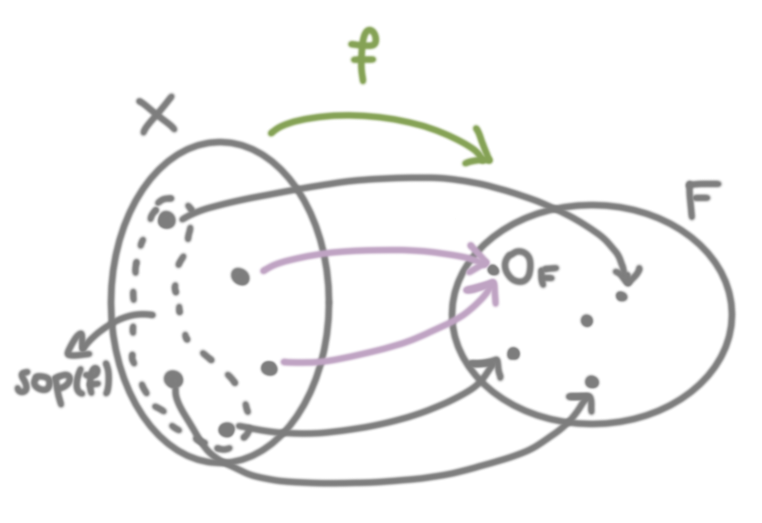
\includegraphics[scale= 1.3]{ 1} 
		\caption{Representación gráfica del soporte de una función.}
\end{marginfigure}
como el conjunto de los puntos del dominio para 
los que $f$ no se anula:
\[
sop(f) :=
\{ x \in X  | \hspace{0.2cm} f(x) \neq 0 \}.
\]

\end{defi}

\begin{ejem}
Tomemos a $X = \IN$. Acostumbramos llamar a los 
elementos de $F^{\IN}$ \textbf{sucesiones en $F$}.
De hecho, dada una función $f \in F^{\IN}$, 
es usual identificarla con el conjunto de sus imágenes:
\[
f = (f_{n})_{n \in \IN}, 
\hspace{0.2cm} \textit{ donde }
f_{n} := f(n).
\]
\hlgray{Ejercicio:} Demuestre que,
si $f = (f_{n})_{n \in \IN} \in F ^{\IN}$ tiene soporte 
finito, entonces $\lim_{n \rightarrow \infty} f(n) = 0$.
¿Se vale la otra implicación?
\diam
\end{ejem}


\begin{defi}
Denotaremos por $F^{(X)}$ al conjunto de las funciones
de $X$ en $F$ que tienen soporte finito, es decir,
\[F^{(X)} := \{ f \in F^{X}  | \hspace{0.2cm}  
|sop(f) < \infty|\}.
\]
\end{defi}


Para lo que sigue, necesitamos que el lector recuerde
(o al menos esté de acuerdo en aceptar como ciertos)
los siguientes hechos:
\begin{itemize}
	\item La cardinalidad del conjunto vacío es $0$.
	El conjunto vacío es el único conjunto de cardinalidad $0$.
	\item Si $A$ y $B$ son dos conjuntos finitos, entonces
	$A \cup B$ es también finito.
	\item Si $A$ está contenido en $B$ y $B$ es finito, entonces
	$A$ también lo es.
\end{itemize}

\begin{prop}
Si $X \neq \emptyset$ y $F$ es un campo, entonces
$F^{(X)}$ es un subespacio de $F^{X}$.
\end{prop}
\noindent
\textbf{Demostración.}
Usemos los criterios dados en la proposición $(*-sub)$
para mostrar que $F^{(X)} \leq F^{X}$.
\begin{enumerate}
	\item Si $\hat{0}: X \longrightarrow F$ es la función
	cero, 
	\[
	sop(\hat{0}) = \{ x \in X  | \hspace{0.2cm} \hat{0}(x) \neq 0\}
	= \emptyset,
	\]
	luego, $\hat{0}$ tiene soporte finito, o sea, 
	$\hat{0} \in F^{(X)}$.
	
	\item Sean $f, g \in F^{(X)}$; veamos que $f + g \in F^{(X)}$.
	Es decir, usando que $f$ y $g$ tienen soporte finito, mostremos
	que $f+g$ también tiene soporte finito.
	Si $sop(f + g) = \emptyset$, acabamos. Supongamos ahora
	que $sop(f+g) \neq \emptyset$. Note que, si 
	$x \in sop(f+g)$, entonces
	\[
	f(x) + g(x) = (f+g)(x) \neq 0,
	\]	
	luego, no ocurre $f(x) = 0 = g(x)$, es decir,
	\[
	x \not\in (sop(f))^{c} \cap (sop(g))^{c},
	\]
	o sea, 
	\[
	x \in sop(f) \cup sop(g).
	\]
	Con esto demostramos la contención
	\[
	sop(f+g) \subseteq sop(f) \cup sop(g).
	\]
	Como $sop(f)$ y $sop(g)$ son, por hipótesis, ambos
	finitos, su unión también lo es, luego
	$sop(f+g)$, por ser subconjunto de un conjunto finito,
	es finito.
	
	\item Sean $f \in F^{(x)}$ y $a \in F$; probemos que
	$af \in F^{(X)}$. Si $a = 0$, 
	$a f = \hat{0} \in F^{(X)}$; supongamos ahora $a \neq 0$.
	\marginnote{Recuerda que, en un campo, el producto de dos
	elementos es cero si y sólo si al menos uno de los dos es cero.}
	Entonces,
	\begin{align*}
	x \in sop(af) & \Leftrightarrow  af(x) \neq 0 \\
	& \Leftrightarrow  a \neq 0 \textit{ y } f(x) \neq 0 \\
	& \Leftrightarrow  f(x) \neq 0 
	\Leftrightarrow x \in sop(f).
	\end{align*}
	Así, $sop(a f) = sop(f)$, luego, $af$ tiene, al igual
	que $f$, soporte finito.
\end{enumerate}

\QEDB
\vspace{0.2cm}

\section{El subespacio generado por un subconjunto y suma de subespacios}


Dado $V$ un $F-$espacio vectorial, 
sea $\{ W_{\alpha} \}_{\alpha \in I}$ una familia no vacía de subespacios
de $V$. A partir de esta familia, ¿cómo podemos construir otro
subespacio de $V$?
Consideremos a la unión e intersección de la familia, o sea,
a los conjuntos

\begin{equation}
	\label{eq: int fam subesp}
	\bigcap_{\alpha \in I} W_{\alpha} :=
\{ x \in V  | \hspace{0.2cm} x \in W_{\alpha} \textit{ para toda }
\alpha \in I  \} \subseteq V,
\end{equation}
y
\begin{equation}
	\label{eq: union fam subesp}
	\bigcup_{\alpha \in I} W_{\alpha} :=
\{ x \in V  | \hspace{0.2cm} x \in W_{\alpha} \textit{ para algúna }
\alpha \in I  \} \subseteq V.
\end{equation}

¿Son estos subespacios de $V$?
Tenemos una
respuesta afirmativa y otra negativa.

\begin{prop}
La intersección \eqref{eq: int fam subesp} de la familia
de subespacios $\{ W_{\alpha} \}_{\alpha \in I}$
de $V$ es un subespacio de $V$.
\end{prop}
\noindent
\textbf{Demostración.}
\begin{itemize}
	\item[i)] Puesto que el cero es elemento de \textit{todo}
	subespacio de $V$, claro que $0 \in W_{\alpha}$ para
	toda $\alpha \in I$, luego, $0 \in \bigcap_{\alpha \in I} W_{\alpha}$
	\item[ii, iii)] Sean $x, y \in \bigcap_{\alpha \in I} W_{\alpha}$,
	$a \in F$; claro que 
	$x+y, ax \in \bigcap_{\alpha \in I} W_{\alpha}$
	pues, dado $\alpha \in I$ un índice cualquiera,
	$x, y \in W_{\alpha}$, luego, como 
	$W_{\alpha}$ es subespacio de $V$, $x+y, ax \in W_{\alpha}$.
\end{itemize}

\QEDB
\vspace{0.2cm}

La demostración anterior fue muy sencilla pues, para
que un vector sea elemento de la intersección
$\bigcap_{\alpha \in I} W_{\alpha}$,
debe estar en \textit{todos} los elementos de la familia a la 
vez, y todos los $W_{\alpha}$ cumplen  
los tres puntos de la proposición (*-sub).
La condición que debe cumplir un vector para estár en la 
unión de la familia es mucho más laxa; es necesario y suficiente
que sea elemento de un solo miembro de la familia
$\{ W_{\alpha} \}_{\alpha \in I}$.
Dados
$x, y \in \bigcup_{\alpha \in I} W_{\alpha}$,
existen $\alpha_{1}, \alpha_{2} \in I$
tales que $x \in W_{\alpha_{1}}$ y 
$y \in W_{\alpha_{2}}$. Nota que \textit{no podemos
decir que $x$ y $y$ son elementos de un mismo subespacio}, luego,
esta información no parece implicar que la suma sea elemento de la 
unión.


\begin{ejem}
(Que muestra que la unión de subespacios puede no ser un subespacio).
Sea $(a, b) \subseteq \IR$ un intervalo abierto cualquiera.
Considere al $\IR-$espacio vectorial
\[
\IR^{(a, b)} = \{ f: (a, b) \longrightarrow
\IR  | \hspace{0.2cm} f \textit{ es función.} \}
\]

Sean 
\[
\mathcal{B}_{a, b} = \{ f \in \IR^{(a, b)}  | \hspace{0.2cm}
f \textit{ es acotada}  \}, \hspace{0.4cm}
\mathcal{C}_{a, b} = \{ f \in \IR^{(a, b)}  | \hspace{0.2cm}
f \textit{ es continua}  \}.
\]
Como sabes por tus cursos de cálculo, estos son subespacios
de $\IR^{(a, b)}$. En la imagen se muestran la gráfica
de una función continua $f$ y una acotada
$g$ en $(a, b)$ para las que la suma no es ni continua ni 
acotada (i.e. tales que $f, g \in \mathcal{B}_{a, b} \cup
\mathcal{C}_{a, b}$ pero $f + g \not\in \mathcal{B}_{a, b}
\cup \mathcal{C}_{a, b}$). 
\begin{figure}[H]
	\sidecaption{
	Con el sumando continuo rompemos la acotación, y con
el sumando acotado, la continuidad.
	\label{fig: 2}
	}
	\centering
	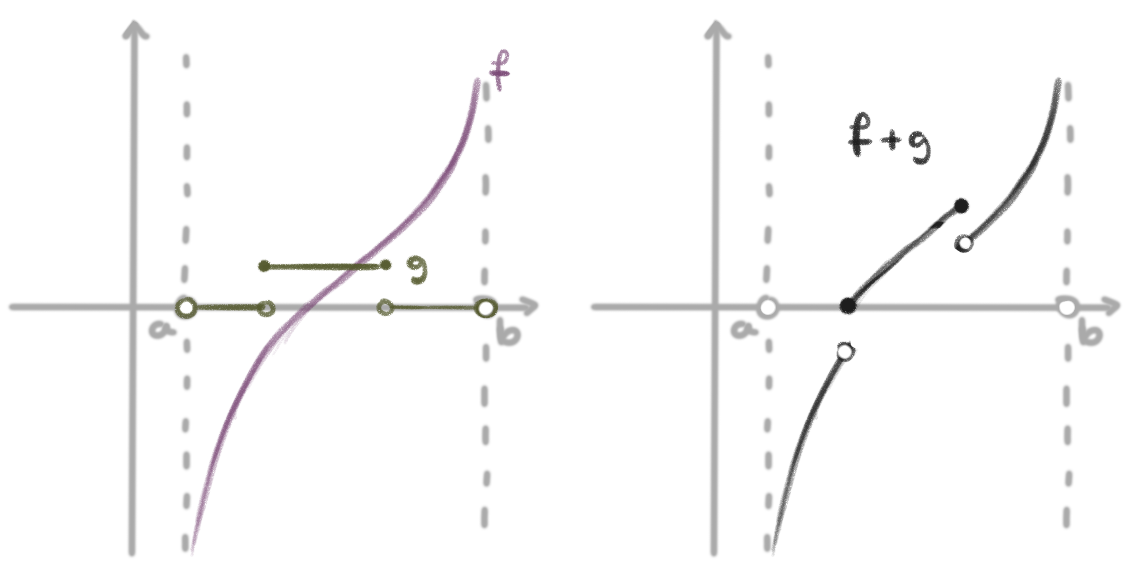
\includegraphics[scale = 2.5]{2} 
\end{figure}	
\diam
\end{ejem}

\hlgray{Ejercicio:} Si $\{ W_{\alpha} \}_{\alpha \in I}$
es una colección de subespacios de $V$ tal que
\[
(\forall i, j \in I)(\exists k \in I): \hspace{0.2cm}
W_{i}, W_{j} \subseteq W_{k},
\]
entonces $\bigcup_{\alpha \in I} W_{\alpha}$ es un subespacio de $V$.


 \begin{center}
 --- * * * ---
 \end{center}
Ahora, dado $V$ un $F-$espacio vectorial, a veces nos interesará
limitarnos a trabajar no con todo el espacio $V$, sino con un 
subconjunto $X$ de este. Como también queremos aprovechar
la estructura algebráica, nos interesará que tal colección $X$
sea, más que subconjunto, subespacio de $V$.
Esto puede ocurrir o no: lo que siempre podemos hacer
es considerar a la familia $\{ W \leq V : 
\hspace{0.2cm} X \subseteq W \}$ de subespacios más pequeños
(en el sentido que están propiamente contenidos en $V$)
que contienen a nuestro conjunto de interés de $X$, y 
``condensar'' a esta familia via su intersección.

\begin{defi}
Sean $V$ un $F-$espacio vectorial, $X \subseteq V$. 
El subespacio
\begin{equation}
	\label{eq: sub generado por X}
	\langle X \rangle := \bigcap \{ W \leq V : \hspace{0.2cm}
	X \subseteq W \},
\end{equation}
o sea, la intersección de la familia de todos los subespacios
de $V$ que contienen a $X$, es llamado el 
\textbf{subespacio de $V$ generado por $X$}.
\end{defi}

\begin{prop}
$\langle X \rangle$ es el menor subespacio de $V$
que contiene a $X$, es decir,
\marginnote{Estamos considerando a la contención de conjuntos
como orden; el que un conjunto $A$ sea menor que un conjunto
$B$ significa que $A$ está contenido en $B$.}
\[
\forall \hspace{0.1cm} W \leq V: \hspace{0.2cm}
X \subseteq W \Rightarrow \langle X \rangle \leq W.
\]
\end{prop}
\noindent
\textbf{Demostración.}
Es clara pues, $\langle X \rangle$, al ser por definición
la intersección de la familia de subespacios que
contienen a $X$, está contenido en cada uno de sus integrantes.

\QEDB
\vspace{0.2cm}

En resumen: si $X$ no es subespacio, siempre podemos
considerar a $\langle X \rangle$, \textit{el menor}
subespacio de $V$ que contiene al conjunto de interés.

\hlgray{Ejercicio:} Demuestre que, si $X \leq V$,
entonces $X = \langle X \rangle$.

\begin{obs}
Por definición,
$\langle \emptyset \rangle $ es la intersección 
de la familia de subespacios que contienen a 
$\emptyset$ - o sea, es la intersección de todos los subespacios
de $V$. Como $\{ 0 \}$ es el menor subespacio de $V$, concluimos que
\[
\langle \emptyset \rangle = \{ 0 \}.
\] 
\end{obs}

En \eqref{eq: sub generado por X} decimos cómo
construir a tal $\langle X \rangle$; el objetivo ahora es dar
una descripción completa de sus elementos, es decir,
dar un criterio concreto en base al cual determinar
cuándo un vector $x$ del espacio pertenece a 
$\langle X \rangle$.

Según la proposición (*-sub), $X$ puede no ser subespacio
por cumplirse al menos una de las tres razones siguientes:
\begin{itemize}
	\item $\hat{0} \not\in X$; corregimos esto agregando
	al vector cero.
	\item Existen $x, y \in X$ tales que 
	$x+y \not\in X$; esto se puede arreglar agregando
	sumas de elementos de $X$.
	\item Existen $a \in F$ y $x \in X$ para los que
	$ax \not\in X$. Para que esto no ocurra, podemos 
	agregar los múltiplos escalares de los elementos de $X$.
\end{itemize}

Parece que el problema de no ser subespacio se arregla
si agregamos sumas finitas de múltiplos escalares de elementos
de $X$ (pues así estamos forzando a que los tres puntos de la 
proposición (*-sub) ocurran). Demos un nombre a tales
sumas de elementos de $X$.

\begin{defi}
Sea $V$ un $F-$espacio vectorial, $X \subseteq V$. Una 
\textbf{combinación lineal} en $V$ de elementos de $X$ es cualquier
vector de la forma
\[
\sum_{i=1}^{n} a_{i}x_{i},
\hspace{0.2cm} \textit{ con }
n \geq 1 \textit{ entero, }
x_{i} \in X, a_{i} \in F
\textit{ para toda } 1 \leq i \leq n.
\] 
\end{defi}

Según la discusión anterior, parece que para ``extender''
a $X$ a un subespacio de la forma mínima, hay que agregar
todas las combinaciones lineales de elementos de $X$, pues con esto
parece quedar asegurada la cerradura bajo suma y multiplicación
por escalares. Confirmamos nuestras sospechas con el siguiente resultado.

\begin{prop}
	\label{prop: caract elementos del subesp generado por X}
Si $\emptyset \neq X \subseteq V$, entonces
$\langle X \rangle$ consta de todas las combinaciones lineales
de elementos de $X$, es decir,
\begin{equation}
	\label{eq: elementos del generado de X}
\langle X \rangle = \left\{ \sum_{i=1}^{n} a_{i}x_{i} | \hspace{0.2cm} 
n \in \IN, x_{i} \in X, a_{i} \in F \hspace{0.2cm} \textit{ para toda }
1 \leq i \leq n \right\}
\end{equation}
\end{prop}
\marginnote{En inglés, al conjunto de la derecha en 
\eqref{eq: elementos del generado de X} se le conoce como
el ``span'' de $X$. La proposición 
\ref{prop: caract elementos del subesp generado por X}
nos dice que el span de un conjunto $X$ es el menor subespacio
que contiene a $X$.}
\noindent
\textbf{Demostración.}
Sea 
\[
\mathcal{A} = \left\{ \sum_{i=1}^{n} a_{i}x_{i} | \hspace{0.2cm} 
n \in \IN, x_{i} \in X, a_{i} \in F \hspace{0.2cm} \textit{ para toda }
1 \leq i \leq n \right\};
\]
veamos que $\mathcal{A} = \langle X \rangle$.
\begin{itemize}
	\item[$\supseteq$]] Claro que $\mathcal{A}$ es subespacio de 
	$V$ (\hlgray{Ejercicio:} compruebe los detalles!). Además, 
	$\mathcal{A}$ contiene a $X$ (pues $x = \sum_{i=1}^{1}1_{F} x \in \mathcal{A}$).
	De esto se deduce que $\langle X \rangle \subseteq \mathcal{A}$.
	
	
	\item[$\subseteq$]] Sea ahora
	$a_{1} x_{1} + \ldots + a_{n} x_{n}$ un elemento genérico 
	de $\mathcal{A}$; mostremos que este es elemento de 
	\textit{cualquier} subespacio $W$ de $V$ que contenga a 
	$X$ - de esto podremos concluir la contención deseada, 
	pues $\langle X \rangle$ \textit{es} la intersección 
	de tales subespacios $W$.
	Sea pues $W \leq V$ con $X \subseteq W$. Como cada
	$x_{i}$ es elemento de $X$, todos serán elementos de 
	$W$, luego, por el lema REF, 
	$a_{1} x_{1} + \ldots + a_{n} x_{n} \in W$.
\end{itemize}

\QEDB
\vspace{0.2cm}

\begin{defi}
Si $\{ W_{\alpha} \}_{\alpha \in I}$ es una familia de subespacios
de $V$, definimos a su suma como el subespacio generado por su unión,
es decir,
\begin{align}
	\label{eq: suma de subespacios}
\sum_{\alpha \in I} W_{\alpha} := &
\left\langle \bigcup_{\alpha \in I} W_{\alpha} 
\right\rangle \nonumber \\
= & \left\{ a_{1}w_{1} + \cdots +
a_{n}w_{n}  | \hspace{0.2cm} n \geq 1, a_{i} \in F,
w_{i} \in \bigcup_{\alpha \in I} W_{\alpha} \right\} \nonumber \\
= & \{ a_{1}w_{1} + \ldots + 
a_{n}w_{n}  | \hspace{0.2cm} n \geq 1,
a_{i} \in F, w_{i} \in W_{\alpha} 
\hspace{0.1cm} \textit{ para alguna } \alpha \in I \}.
\end{align}
\end{defi}

\hlgray{Ejercicio:} Demuestre que una forma equivalente de
escribir al subespacio \eqref{eq: suma de subespacios}
es como
\begin{equation}
	\label{eq: suma de subespacios simplificado}
	\sum_{\alpha \in I} W_{\alpha} =
	\{ w_{1} + \cdots + w_{n} : \hspace{0.2cm}
	n \geq 1, w_{i} \in W_{i} \hspace{0.1cm} \forall 1 \leq i \leq n  \}.
\end{equation}


Recapitulemos: dados $W_{1}, W_{2} \leq V$,
\begin{itemize}
	\item $W_{1} \cap W_{2}$ es un subespacio de $V$,
	\item $W_{1} \cup W_{2}$ es subespacio si y sólo si 
	$W_{1} \subseteq W_{2}$ o bien $W_{2} \subseteq W_{1}$. Nota
	que el resultado de esta operación no da lugar a un nuevo
	subespacio de $V$.
	\item El menor subespacio de $V$ que contiene a $W_{1}$
	y $W_{2}$ es su suma, o sea, 
	\[
	W_{1} + W_{2} = \{ w_{1} + w_{2}  | \hspace{0.2cm} 
	w_{1} \in W_{1}, w_{2} \in W_{2} \}.
	\]
\end{itemize}

\begin{defi}
Si $X \subseteq V$ es tal que $\langle X \rangle = V$,
decimos que \textbf{$X$ genera al espacio $V$}.
\end{defi}
Es decir, $X$ genera a a $V$ si no hay subespacios propios
de $V$ que contengan a $X$; esto, según la proposición
\ref{prop: caract elementos del subesp generado por X}, significa que
\textit{todo elemento de $V$ puede expresarse como combinación
lineal finita de elementos de $X$}.

\subsection{Suma directa de subespacios}

Sean $V$ un $F$-espacio vectorial, 
$\{ W_{i} \}_{i=1}^{n}$ una familia finita de subespacios
de $V$. Por la proposición 
\ref{prop: caract elementos del subesp generado por X}
sabemos que \textit{todo} elemento de 
su suma es de la forma 
$w_{1} + \ldots + w_{n}$, con $W_{i} \in W_{i}$ para
$1 \leq i \leq n$.

\begin{ejem}
Sea el $\IR-$espacio vectorial $\IR^{3}$. Considere a los subespacios
\[
W_{1} = \{ (a, b, 0)  | \hspace{0.2cm} a, b \in \IR \}
\leq \IR^{3},
\]
\[
W_{2} = \{ (0, c, d)  | \hspace{0.2cm} c, d \in \IR \}
\leq \IR^{3}.
\]
Es claro que $\IR^{3} = W_{1} + W_{2}$; de hecho, dado
$(x, y, z) \in \IR^{3}$ un vector cualquiera del espacio, 
para toda $\alpha \in \IR$ se tiene que
\marginnote{Las entradas cero de los elementos de $W_{1}$
y $W_{2}$ determinan las entradas $x$ y $z$ en la ecuación
\eqref{eq: 1, 21 Ag}, 
pero en las entradas centrales tenemos libertad de elección
-esto se ve reflejado por el parámetro $\alpha$.}
\begin{equation}
	\label{eq: 1, 21 Ag}
	(x, y, z) = (x, \alpha y, 0) + 
(0, (1-\alpha)y, z).
\end{equation}

Esto muestra que hay \textit{una infinidad} de formas
de expresar a un 
vector $(x, y, z) \in \IR^{3}$ como suma
de elementos de $W_{1} \cup W_{2}$.

Considere ahora a los subespacios
\[
V_{1} = \{ (a, 0, 0)  | \hspace{0.2cm} a\in \IR \},
\]
\[
V_{2} = \{ (0, b, 0)  | \hspace{0.2cm} b\in \IR \},
\]
\[
V_{1} = \{ (0, 0, c)  | \hspace{0.2cm} c\in \IR \}.
\]
Claro que $\IR^{3} = V_{1} + V_{2} + V_{3}$; dado
$(x, y, z) \in \IR^{3}$ cualquiera,
\[
(x, y, z) = (x, 0, 0) + (0, y, 0) + (0, 0, z).
\]
Una representación de esta forma es única. Por ejemplo,
el que las primeras entradas de los últimos dos sumandos
deban ser cero (por definición de $V_{1}$ y $V_{2}$)
forza que la primera entrada del primer sumando sea $x$.
\diam
\end{ejem}

\begin{defi}
Sea $\{ W_{i} \}_{i=1}^{n}$ una familia finita de subespacios
de $V$. 
\marginnote{El símbolo $\oplus$ es usado para representar
una propiedad del espacio suma $\sum_{i=1}^{n} W_{i}$,
a saber, la unicidad de las representaciones de sus elementos
como sumas de vectores en $\bigcup_{i=1}^{n}W_{i}$.}
El subespacio suma $\sum_{i=1}^{n} W_{i}$
es llamada una \textbf{suma directa} si cada uno de sus
elementos tiene una única representación de la forma
\[
w_{1} + \cdots  + w_{n}, 
\hspace{0.2cm} \textit{ con }
w_{i} \in W_{i}.
\]
En este caso, al subespacio $\sum_{i=1}^{n}W_{i}$
se le denota por
\[
W_{1} \oplus \cdots \oplus W_{n}.
\]
\end{defi}

\begin{prop}
	\label{prop: suma directa sii interseccion cero}
Sean $U, W$ subespacios de $V$. La suma
$U+ W$ es directa si y sólo si $U \cap W = \{ \hat{0} \}$.
\end{prop}
\noindent
\textbf{Demostración.}
\begin{itemize}
	\item[$\Rightarrow$]] Si existe $x \in U \cap W$
	con $x \neq \hat{0}$, entonces, 
	\[
	x = \hat{0} + x, \hspace{0.2cm} \textit{ con }
	\hat{0} \in U, x \in W,
	\]
	y 
	\[
	x = x + \hat{0}, \hspace{0.2cm} \textit{ con }
	x \in U, \hat{0} \in W,
	\]
	luego, la suma $U + W$ no es directa.
	
	\item[$\Leftarrow$]] Sea $x \in U + W$; sean
	$u_{1}, u_{2} \in U$ y $w_{1}, w_{2} \in W$ tales que
	\[
	u_{1} + w_{1} = x = u_{2} + w_{2}.
	\]
	Entonces, 
	\[
	u_{1} - u_{2} = w_{2} - w_{1} \in U \cap W = \{ 0 \},
	\]
	o sea, $u_{1} = u_{2}$ y $w_{1} = w_{2}$.
	
	
\end{itemize}

\QEDB
\vspace{0.2cm}

Note lo siguiente: según la proposición 
(*-sub), todos los subespacios tienen en común al 
neutro $\hat{0}$ del espacio, luego, no tiene sentido
buscar subespacios disjuntos. Lo más disimiles que pueden
llegar a ser $U, W \leq V$ es que su intersección sea
$\{ 0 \}$. Esto, según la proposición 
\ref{prop: suma directa sii interseccion cero}, 
equivale a que la suma $U + W$ sea directa.


\begin{center}
Suma de subespacios $\sim$ Unión de subconjuntos \\
Suma directa de subespacios 
$\sim$ Unión disjunta de subconjuntos
\end{center}

Note que en la proposición \ref{prop: suma directa sii interseccion cero}
estamos lidiando sólo con dos subespacios. ¿Podemos generalizar
este resultado para la suma de $n$-subespacios? ¿Será cierto que
la suma $\sum_{i=1}^{n} W_{i}$ es directa si y sólo si 
la intersección $\bigcap_{i = 1}^{n} W_{i}$ es $\{ \hat{0} \}$?
La respuesta es \textbf{no} (c.f. ejercicio
\ref{ej: de la suma directa}).


\section{Caso práctico: Representación de información nutricional}

Veamos cómo los conceptos introducidos pueden ser de utilidad
para modelar y resolver una problemática de la vida real.

Supongamos que a una nutrióloga le interesa
la ingesta de 
\begin{itemize}
	\item calorías
	\item agua
	\item hidratos de carbono 
	\item fibra
	\item grasas, y 
	\item proteinas
\end{itemize}
que un paciente puede obtener al consumir frutas de cierto
grupo de interés (por ejemplo, las frutas que puede encontrar
a precio accesible en su entorno). Sus datos iniciales son
los valores de dichos componentes presentes en las frutas
de interés, datos presentados en forma de tabla como
se muestra a continuación.

\begin{figure}[H]
	\sidecaption{
	Fuente: 
	\url{gruporem-ucam.com}
	\label{fig: tabla frutas}
	}
	\centering
	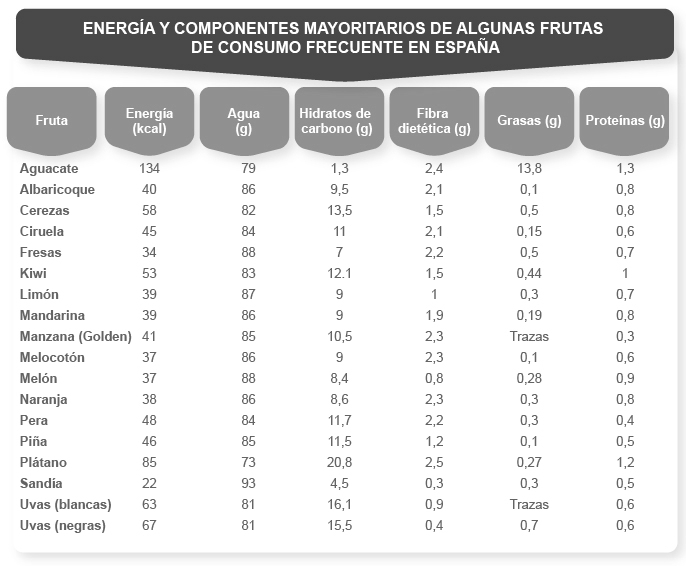
\includegraphics[scale = 0.5]{tablaFrutas} 
\end{figure}	

Algunos de sus pacientes son alérgicos a las frutas de
su lista; digamos que su nuevo paciente no puede 
comer manzanas. La nutrióloga se pregunta si es posible
sustituir los nutrientes aportados por una manzana
con otras frutas de la lista y, si la respuesta es afirmativa,
quisiera dar explícitamente combinaciones de frutas que 
aporten lo mismo que aportaba una cierta cantidad de manzanas
(que no pueden ser incluidas en la dieta del paciente). 
¿Cómo podemos modelar esta situación?

Podemos representar nuestros datos iniciales como
vectores de $\IR^{6}$; por ejemplo, el vector
nutricional de una manzana sería
\[
x_{manzana} = (41, 85, 10.5, 2.3, 0, 0.3)
\in \IR^{6}.
\]
Definamos a $\mathcal{A}$ como el subconjunto de $\IR^{6}$
que consta de todos los vectores fruta,
\[
\mathcal{A} = \{ x_{aguacate}, x_{albaricoque}, \ldots , x_{uvasB},
x_{uvasN} \}.
\]

Nota que, en este contexto, las combinaciones lineales
con coeficientes naturales tienen una interpretación física; por
ejemplo, el vector
\[
2x_{pera} + 5 x_{fresa} + 3 x_{cereza}
\]
representa la información nutrimental de 2 peras,
5 fresas y 3 cerezas (luego, la cantidad de calorías y componentes
que alguien estaría obteniendo al consumir esta cantidad de frutas).

El problema de la nutrióloga queda expresado en términos
de álgebra lineal como sigue:
¿es $x_{manzana}$ elemento del subespacio de $\IR^{6}$ generado
por los vectores $x_{aguacate}, x_{albaricoque}, \ldots ,
x_{uvaB}, x_{uvaN}$? Nota que, implícitamente,
el problema nos permite limitarnos al conjunto de
las combinaciones lineales finitas de los vectores fruta
(menos el vector manzana) y no considerar a todo $\IR^{6}$
(para este problema, no nos interesan vectores que no sean combinaciones
lineales de vectores fruta). La teoría estudiada antes nos asegura que
\begin{itemize}
	\item Tal conjunto de combinaciones de vectores fruta
	es un subespacio de $\IR^{6}$ y,
	\item de hecho, es el menor subespacio de $\IR^{6}$ que contiene 
	a los vectores fruta menos el manzana.
\end{itemize}

La pregunta de la nutrióloga queda entonces expresada en ver si ocurre
\[
x_{manzana} \in \langle \mathcal{A} - \{ x_{manzana} \} \rangle
\]
o no.
\marginnote{No nos interesan todos los elementos de $\IR^{6}$, sino
sólo aquellos que sean combinaciones lineales de vectores fruta;
estamos reemplazando a nuestro espacio de trabajo $\IR^{6}$
por $\langle \mathcal{A} \rangle$.}

Observa que los vectores son mucho más que una forma conveniente de 
almacenar información: podemos hacer operaciones de ellos e
interpretarlas en el contexto del 
problema físico planteado.

Con las definiciones e ideas que planteamos en los siguientes capítulos,
podremos 
\begin{itemize}
	\item Determinar cuándo existen combinaciones de frutas
	que aporten lo mismo que cierta cantidad de manzanas,
	\item Decir si hay una única forma o varias de expresar manzanas
	en términos de combinaciones lineales de frutas específicas
	\item Usar argumentos de dimensionalidad para determinar
	cuándo subconjuntos de frutas son suficientes para
	sustituir a todas las demás
\end{itemize}

Es fácil pensar requerimientos razonables
que complicarían aún más la situación; por ejemplo, considera que,
en un escenario realista, 
\begin{itemize}
	\item Un paciente podría tener no solo posibles alergias
	como limitantes para definir una dieta, sino también 
	un presupuesto mensual al que deba apegarse, presupuesto
	que podría reducir aún más las opciones o cantidades
	de fruta que puede consumir (por ejemplo, esto podría implicar
	que combinaciones lineales que contengan al vector
	$x_{aguacate}$ sólo sean consideradas cuando su coeficiente
	-i.e. el escalar por el que se multiplica a $x_{aguacate}$ - 
	no sea mayor a cierto valor).
\end{itemize}



\begin{figure}[H]
\centering\captionsetup{format = hang}
	\begin{measuredfigure}
		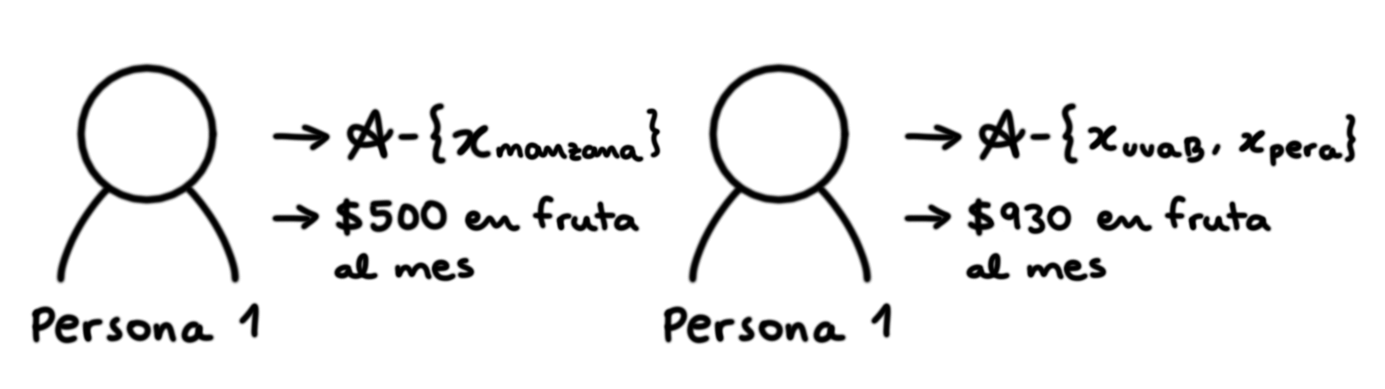
\includegraphics[scale=2]{3} 
		\caption{Cada paciente tiene sus necesidades personales,
		por ejemplo, las frutas a las que es alérgico (o que no le
		gustan, y quiere evitar en su dieta) y su presupuesto mensual.
		Esto cambia el espacio de combinaciones lineales a considerar
		para cada uno, y las combinaciones lineales aceptables.}
 	\end{measuredfigure}
 \end{figure}

Incluso en esta situación tan simplificada, vemos la utilidad
de usar el marco teórico ofrecido por el álgebra lineal para
modelar la situación; con los conocimientos de los próximos
capítulos seremos capaces de resolver los problemas
aquí planteados. 
\section{Ejercicios I}
En lo que sigue, a menos que se indique lo contrario,
$V$ es un $F-$espacio vectorial.
Los ejercicios marcados con el símbolo
$\mathbat$ son obligatorios para los estudiantes de matemáticas,
pero opcionales para los de actuaría.

\begin{ej}
    Demuestre que
    \[
    W_{1} = \{ (a_{1}, \ldots , a_{n}) \in \IR^{n} : \hspace{0.2cm} 
    a_{1} + \cdots + a_{n} = 0\}
    \]
    es un subespacio de $\IR^{n}$, pero que 
    \[
    W_{1} = \{ (a_{1}, \ldots , a_{n}) \in \IR^{n} : \hspace{0.2cm} 
    a_{1} + \cdots + a_{n} = 1\}
    \]
    no lo es.
\end{ej}

\begin{ej}
    Demuestre que un subconjunto $W$ de un espacio vectorial $V$
    es un subespacio de $V$ si y sólo si
    \begin{enumerate}
        \item $0 \in W$, y
        \item para todo $a \in F$ y $x, y \in W$, se tiene que
        $ax + y \in W$.
    \end{enumerate}
\end{ej}

\begin{ej}
\hlpink{\textbf{El $F-$espacio vectorial de polinomios con coeficientes en
un campo $F$:}}
Sea $F$ un campo. Un \textbf{polinomio con coeficientes en el campo $F$}
es una función $f : F \longrightarrow F$ de la forma
\begin{align}
	\label{eq: pol f}
f(x) = & a_{n}x^{n} + a_{n-1}x^{n-1} + \cdots + a_{1}x + a_{0} \nonumber \\
= & \sum_{i=0}^{n} a_{i}x^{i},  
\end{align}
\marginnote{Haciendo $F = \IR$, el polinomio
$f(x) = x^{2}-1$ tiene grado dos y es mónico, $f(x) = 4$
tiene grado cero.}
donde $n \geq 1$ entero y $a_{0}, a_{1}, \ldots , a_{n} \in F$. 
A los $a_{i}$ se les conoce como
\textbf{coeficientes del polinomio}. Si todos los coeficientes
son cero, decimos que $f$ es el \textbf{polinomio cero}, 
y definimos a su \textbf{grado} como $-1$.
Si $a_{n} \neq 0$, decimos que el grado del polinomio
es $n$ y $a_{n}$ es su \textbf{coeficiente principal}.
Todo polinomio cuyo coeficiente principal sea $1$ será llamado
\textbf{mónico}.

Dos polinomios $f(x)$ y $g(x)$ son iguales si y sólo si 
tienen el mismo grado y sus correspondientes coeficientes
son iguales.

Sea
\[
F[x] := \{ f \in F^{F}  | \hspace{0.2cm} f \textit{ es un polinomio} \}
\]
el conjunto de todos los polinomios con coeficientes en $F$.
Definimos 
\marginnote{
Puedes encontrar esta definición
del espacio vectorial de polinomios en el Friedberg, p.10. 
Te recomiendo que estudies también cómo $F[x]$ es 
esencialmente igual al espacio $F^{(\IN)}$ de sucesiones
en $F$ con soporte finito.}
\begin{enumerate}
	\item La suma de dos polinomios
	\[
	f(x) = \sum_{i=0}^{n} a_{i}x^{i},
	\hspace{0.2cm}
	g(x) = \sum_{i=0}^{m} b_{i}x^{i},
	\hspace{0.3cm} a_{n}, b_{m} \neq 0
	\]
	como sigue; sin pérdida de generalidad, supongamos que
	$n \leq m$. La suma de $f$ con $g$ es
	\[
	(f+g)(x) = \sum_{i=0}^{m} (a_{i} + b_{i}) x^{i},
	\]
	donde, para $n \leq i \leq m$, definimos $a_{i} = 0$.
	
	\item La multiplicación escalar de un polinomio cualquiera
	\eqref{eq: pol f} por un escalar $\alpha \in F$ como
	el polinomio
	\[
	(\alpha f )(x) = \sum_{i=0}^{n} (\alpha a_{i}) x^{i}
	\]
\end{enumerate}


\begin{itemize}
	\item Demuestre que $F[x]$ es, con la suma y la multiplicación
	escalar definida arriba, un $F$-espacio vectorial.
	\item Sea
	\[
	M[x] = \{ f \in \IR[x] : \hspace{0.2cm} f \textit{ es mónico} \}.
	\]
	¿Es $M[x] \leq \IR[x]$?
	\item ¿Es $\IR[x] - M[x] \leq \IR[x]$?
	\item Para $n \geq 0$, Sea
	\[
	\IR_{n}[x] = \{ f \in \IR[x]  | \hspace{0.2cm} \textit{el grado de f es 
	menor o igual a n}  \}.
	\]
	Demuestre que $\IR_{n}[x] \leq \IR[x]$. Muestre además que
	$\{ 1, x, x^{2}, \ldots , x^{n} \}$ genera a $\IR_{n}[x]$.
\end{itemize}
\end{ej}

\begin{ej}
\hlpink{\textbf{El $F-$espacio vectorial de matrices de dimensión $m \times n$
con coeficientes en $F$}}: 

Dado un campo $F$, una \textbf{matriz 
$m \times n$ dimensional con coeficientes en $F$}
es una función de la forma
\[
A : \{ 1, \ldots, m \} \times 
\{ 1, \ldots, n \} \longrightarrow F.
\]
Normalmente abreviamos
\[
A(i, j) = a_{i,j},
\hspace{0.2cm} 1 \leq i \leq m, \hspace{0.1cm}
1 \leq j \leq n,
\]
y representamos a la matriz $A$ como un arreglo rectangular
\[
A = (a_{ij}) =
\begin{pmatrix}
a_{11} & a_{12} & \cdots & a_{1n} \\ 
a_{21} & a_{22} & \cdots & a_{2n} \\
\vdots & \vdots & \vdots & \vdots \\
a_{m1} & a_{m2} & \cdots & a_{mn}
\end{pmatrix}.
\]
Definimos tanto la suma de matrices como la multiplicación
escalar entrada a entrada: para cualesquiera
$A = (a_{ij}), B = (b_{ij})$, $\alpha \in F$,
\[
A + B := (a_{ij} + b_{ij}), 
\hspace{0.2cm}
\alpha A := (\alpha a_{ij}).
\]

\begin{itemize}
	\item Demuestre que el conjunto $M_{m \times n}(F)$
	de las matrices $m \times n$ dimensionales con entradas en 
	$F$ y las operaciones definidas arriba es un $F-$espacio vectorial.
	\item Demuestre que las matrices 
	$$\begin{pmatrix}
1 & 0 \\
0 & 0 
\end{pmatrix},
\hspace{0.1cm}
\begin{pmatrix}
0 & 1 \\
0 & 0 
\end{pmatrix},
\hspace{0.1cm}
\begin{pmatrix}
0 & 0 \\
1 & 0 
\end{pmatrix},
\hspace{0.1cm}
\begin{pmatrix}
0 & 0 \\
0 & 1 
\end{pmatrix}
$$
generan a $M_{2 \times 2}(F)$.
	\item Demuestre que
	\[
	D_{n} := \{ A=(a_{ij}) \in M_{n \times n}(F)  | \hspace{0.2cm}
	i \neq j \Rightarrow a_{ij} = 0  \},
	\]
	el conjunto de las matrices diagonales $n-$dimensionales,
	es un subespacio de $M_{n \times n}(F)$.
	\item Si 
	\[
	TS_{m,n} := \{ A=(a_{ij}) \in M_{m \times n}(F)  | \hspace{0.2cm} 
	i > j \Rightarrow a_{ij} = 0 \}
	\]
	es el conjunto de las matrices triangulares superiores
	de dimensión $m \times n$, demuestre que
	$TS_{m,n} \leq M_{m \times n}(F)$.
\end{itemize}
\end{ej}



\begin{ej}
    Demuestre que un subconjunto
    $W$ de $V$ es subespacio de $V$ si y sólo si coincide con el subespacio
    que genera en $V$, es decir, que
    \[
    W \leq V \Leftrightarrow
    W = \langle W \rangle
    \]
\end{ej}

\begin{ej}
    Si $X$ y $Y$ son subespacios1 de $V$, demuestre que
    \[
    \langle X \cup Y \rangle =
    \langle X \rangle + \langle Y \rangle
    =
    \langle \langle X \rangle \cup \langle Y \rangle \rangle
    \]
    Pista: para la segunda igualdad, simplemente use la definición de 
    suma de subespacios.
\end{ej}

\begin{ej}
($\mathbat$) De un ejemplo de un subconjunto no vacío
$U$ de $\IR^{2}$ que sea cerrado bajo multiplicación escalar,
pero que no sea subespacio de $\IR^{2}$.
\end{ej}

\begin{ej}
($\mathbat$) Si $W$ es un subespacio de $V$, describa
al subespacio $W + W$.
\end{ej}

\begin{ej}
    \label{ej: suma directa sii unicidad de representación del cero}
    Si $\{ W_{i} \}_{i=1}^{n}$ es una familia de subespacios de $V$,
    demuestre que las siguientes proposiciones son equivalentes:
    \begin{itemize}
        \item La suma $\sum_{i=1}^{n} W_{i}$ es directa.
        \item Si los vectores $w_{i} \in W_{i}$ ($1 \leq i \leq n$)
        son tales que $w_{1} + \cdots + w_{n} = 0$, entonces 
        toda $w_{i}$ es cero.
    \end{itemize}
    Es decir, demuestre que determinar si representaciones de la forma
    $w_{1} + \cdots + w_{n}$ con $w_{i} \in W_{i}$ son únicas equivale
    a ver la unicidad de la representación sólo del vector cero como suma
    de elementos de $\cup W_{i}$.
\end{ej}

\begin{ej}
	\label{ej: de la suma directa}
    Use a los subespacios
    \[
    W_{1} = \{ (x, y, 0) \in  \IR^{3} : \hspace{0.2cm} x, y \in \IR \},
    \]
    \[
    W_{2} = \{ (0, 0, x) \in  \IR^{3} : \hspace{0.2cm} x \in \IR \},
    \]
    \[
    W_{1} = \{ (0, x, x) \in  \IR^{3} : \hspace{0.2cm} x \in \IR \}
    \]
    de $\IR^{3}$ para dar un ejemplo de una familia de subespacios para la
    que, a pesar de que la intersección es $\{0\}$, la suma no es directa.
    Pista: para facilitarle el trabajo, use el ejercicio 
    \ref{ej: suma directa sii unicidad de representación del cero}.
\end{ej}

\begin{ej}
Si
\[
W_{1} = \{ (a_{1}, \ldots , a_{n}) \in F^{n}  | \hspace{0.2cm} 
a_{1} = 0 \},
\]
\[
W_{2} = \{ (a_{1}, \ldots , a_{n}) \in F^{n}  | \hspace{0.2cm} 
a_{2} = \cdots = a_{n} = 0 \},
\]
demuestre que $F^{n} = W_{1} \oplus W_{2}$.
\end{ej}


\begin{ej}
Sean $X, Y \subseteq V$. Demuestre que
\begin{itemize}
	\item Si $X \subseteq Y$ entonces $\langle X \rangle \leq 
	\langle Y \rangle$.
	\item Si $X \subseteq Y$ y $\langle X \rangle = V$,
	entonces $\langle Y \rangle = V$.
	\item $\langle X \cap Y \rangle \subseteq \langle X 
	\rangle \cap \langle Y \rangle$. Busque un ejemplo en el que
	se de la igualdad y otro en el que la contención sea propia.
\end{itemize}
\end{ej}

\begin{ej} ($\mathbat$)
Sea $b \in \IR$. Defina a la familia
\[
\mathcal{I}_{b} := \left\{
f \in \IR^{[0, 1]}: \hspace{0.2cm}
\int_{0}^{1} f(x) dx = b
\right\}.
\]
Demuestre que $\mathcal{I}_{b}$ es subespacio de $\IR^{[0,1]}$
si y sólo si $b = 0$.
\end{ej}

\begin{ej}
($\mathbat$)
Sea $A \neq \emptyset$ un conjunto cualquiera, $\IZ_{2} = \{ 0, 1 \}$
el campo de los enteros módulo $2$.

Podemos identificar a todo 
subconjunto $B \subseteq A$ con su \textbf{función característica},
es decir, la función $\chi_{B} : A \longrightarrow \IZ_{2}$ definida como
\begin{align*}
 \chi_{B}(x)= \begin{cases}
 1 & \textit{ si } x \in B, \\
 0 & \textit{ si } x \not\in B;
 \end{cases}
 \end{align*}
recíprocamente, toda función $f : A \longrightarrow \IZ_{2}$ 
induce un subconjunto de $A$ como 
\[
B = \{ x \in A : \hspace{0.2cm} f(x) = 1 \}.
\] 
Note que estos procesos son uno el inverso del otro, y que ellos
nos permiten establecer una biyección entre $\mathcal{P}(A)$
-el conjunto potencia de $A$- y el conjunto $\IZ_{2}^{A}$
de funciones de $A$ en $\IZ_{2}$. En la sección 
\ref{subsection: espacios vect de funciones}
vimos cómo dotar a $\IZ_{2}^{A}$ de estructura de 
$\IZ_{2}-$espacio vectorial.

Dados $\alpha \in \IZ_{2}$,
$f, g \in \IZ_{2}^{A}$, si $B$ y $C$ son los subconjuntos
de $A$ que estas funciones inducen,
\begin{itemize}
	\item ¿Qué subconjunto de $A$ induce la función suma $f+g$?
	\item ¿Cuál es el subconjunto de $A$ inducido por la función
	cero $\hat{0} : A \longrightarrow \IZ_{2}$?
	\item ¿Qué subconjunto de $A$ induce $-f$?
	\item ¿Cuál induce $\alpha f$?
	\item Si $\{ B_{i} \}_{i \in I}$ es una familia de subespacios
	de $A$ tal que $\{ \chi_{B_{i}}  | \hspace{0.2cm} 
	i \in I \}$ genera al $\IZ_{2}-$espacio vectorial 
	$\IZ_{2}^{A}$, demuestre que $A = \bigcup_{i \in I} B_{i}$.
\end{itemize}
  
\end{ej}
\section{Dependencia e independencia lineal}

\begin{defi}
	\label{def: ld y li}
Sea $V$ un $F-$espacio vectorial. Decimos que $S \subseteq V$
es \textbf{linealmente dependiente} si existe un número
finito de vectores distintos entre si $x_{1}, \ldots , x_{n} \in S$
y escalares $a_{1}, \ldots , a_{n} \in F$ no todos cero
\marginnote{Abreviamos los términos linealmente dependiente
(resp. independiente) como \textbf{l.d.} (resp. \textbf{l.i.}).}
tales que 
\[
\sum_{i=1}^{n} a_{i}x_{i} = \hat{0}.
\]
Si $S$ no es linealmente dependiente, diremos que es
\textbf{linealmente independiente}.
\end{defi}

En la definición \ref{def: ld y li}
pedimos
\begin{itemize}
	\item que los vectores $x_{i}$ sea distintos entre sí, y
	\item que al menos uno de los escalares $a_{i}$ sea no cero,
\end{itemize}
pues las igualdades
	\[
	1_{F} x + (-1_{F}) x = x - x = \hat{0}
	\]
	y
	\[
	0_{F} x = \hat{0},
	\]
	son ciertas \textit{para todo $x \in V$}, ¡no las vamos a usar
	para definir un nuevo concepto!
	
Si un conjunto finito $S = \{ x_{1}, \ldots , x_{n} \}$
es l.d.(resp. l.i.), acostumbramos decir que los vectores
$x_{1}, \ldots , x_{n}$ son l.d. (resp. l.i.).


\hlgray{Ejercicio:}
Niegue la definición de dependencia lineal dada en 
\ref{def: ld y li} para obtener la definición de independencia lineal.

\begin{ejem}
\begin{itemize}
	\item Por vacuidad, el conjunto vacío es linealmente independiente
	\item Todo subconjunto de $S$ que que contenga al cero es
	linealmente dependiente
\end{itemize}
\diam

\end{ejem}
\hlgray{Ejercicio:} demuestre a detalle los puntos del ejemplo anterior.

\hlgray{Ejercicio:} demuestre que, dados $S \subseteq T \subseteq V$,
\begin{itemize}
	\item si $T$ es l.i., entonces $S$ es l.i.
	\item si $S$ es l.d., entonces $T$ es l.d. 
\end{itemize}

\hlgray{Ejercicio:} demuestre que 
si $x_{1}, \ldots , x_{n}$ distintos entre sí son l.i. y
$a_{1} x_{1} + \cdots + a_{n} x_{n} = \hat{0}$, entonces todos
los escalares $a_{i}$ son iguales a cero.


\begin{prop}
	\label{prop: ld equiv fried y hugo}
\marginnote{El enunciado dado en la proposición 
\ref{prop: ld equiv fried y hugo} es
la definición de dependencia lineal manejada por Hugo Rincón (REF).}
$S \subseteq V$ es linealmente dependiente si y sólo si 
existe $x \in S$ tal que $x \in \langle S - \{ x \} \rangle$.
\end{prop}
\noindent
\textbf{Demostración.}
\begin{itemize}
	\item[$\Rightarrow$]] Sean $x_{1},\ldots , x_{n} \in S$
	distintos entre sí y $a_{1}, \ldots , a_{n}$ escalares no cero 
	tales que $\sum_{i=1}^{n} a_{i}x_{i} = \hat{0}$.
	Sin pérdida de generalidad, supongamos que 
	$a_{1} \neq 0$. Entonces,
	\[
	a_{1}x_{1} = - \sum_{i=2}^{n} a_{i}x_{i} \in 
	\langle S - \{ x_{1} \} \rangle,
	\]
	luego, $x_{1} \in \langle S -\{ x_{1} \} \rangle$.
	\item[$\Leftarrow$]] Sea $x \in S$ tal que 
	$x \in \langle S - \{ x \} \rangle$. Sean pues
	$x_{1}, \ldots ,x_{n} \in S - \{ x \}$ distintos
	entre si 
	tales que $x = \sum_{i = 1}^{n} a_{i}x_{i}$. Restando $x$
	de ambos lados de la igualdad llegamos a que
	\[
	\hat{0} = \sum_{i = 1}^{n} a_{i}x_{i} - x
	= \sum_{i = 1}^{n} a_{i}x_{i} + (-1_{F}) x.
	\]
	(c.f. prop REF). Como $-1_{F} \neq 0_{F}$, esta última
	igualdad muestra que $S$ es linealmente dependiente.
	
\end{itemize}

\QEDB
\vspace{0.2cm}

\begin{prop}
	\label{prop: singulete x l.i. sii x no cero}
Un singulete $\{ x \} \subseteq V$ es linealmente independiente en $V$
si y sólo si $x \neq \hat{0}$.
\end{prop}
\noindent
\textbf{Demostración.}
En efecto, según la proposición
\ref{prop: ld equiv fried y hugo},
$\{ x \}$ es linealmente dependiente si y sólo si 
$x \in \langle \{ x \} - \{ x \} \rangle = 
\langle \emptyset \rangle = \{ 0 \}$, 
o sea, si y sólo si $x$ es el vector cero.
\QEDB
\vspace{0.2cm}


\begin{prop}
$S \subseteq V$ es linealmente dependiente si y sólo si 
existe $x \in S$ tal que $\langle S \rangle = 
\langle S - \{ x \} \rangle$.
\end{prop}
\noindent
\textbf{Demostración.}
Usaremos la equivalencia probada en la proposición
\ref{prop: ld equiv fried y hugo}.
\begin{itemize}
	\item[$\Rightarrow$]] Sea $x \in S$ tal que 
	$x \in \langle S - \{ x \} \rangle$.
	 Como $S - \{ x \}$ está contenido 
	en $S$, trivialmente $\langle S - \{ x \} \rangle$
	está contenido en $\langle S \rangle$. 
	La otra contención se 
	da también pues, por poder $x$ expresarse como combinación lineal 
	de elementos de $S - \{ x \}$, en cualquier combinación lineal
	de elementos de $S$ se puede reemplazar a $x$ con múltiplos
	escalares de $S-\{ x \}$, es decir, todo elemento
	de $\langle S \rangle$ es elemento de 
	$\langle S - \{ x \} \rangle$.
	\item[$\Leftarrow$]]  Si existe $x \in S$
	tal que $\langle S \rangle = 
	\langle S - \{ x \} \rangle$, entonces
	\[
	x \in S \subseteq \langle S \rangle = 
	\langle S - \{ x \} \rangle.
	\]
	
\end{itemize}

\QEDB
\vspace{0.2cm}

Este resultado nos indica que, cuando un conjunto $S$
es l.d., hay al menos un vector 
que es \textbf{redundante}, en el sentido en que hay otros
vectores en $S$ que pueden reemplazar a $x$ para generar
al span de $S$; el quitar a $x$ de $S$ no implica una pérdida
de información.

\begin{prop}
	\label{prop: li caracter finito}
Dado $S \subseteq V$, son equivalentes las siguientes proposiciones:
\marginnote{La proposición \ref{prop: li caracter finito} dice que
ser l.i. es una \textbf{propiedad de carácter finito}
(ref wiki).}
\begin{itemize}
	\item $S$ es linealmente independiente
	\item Todo subconjunto finito de $S$ es linealmente independiente.
\end{itemize}
\end{prop}
\noindent
\textbf{Demostración.}

\begin{itemize}
	\item[$\Rightarrow$]] En general, todo subconjunto de un
	conjunto linealmente independiente es también linealmente
	independiente.
	\item[$\Leftarrow$]] Por contrapuesta. Sea
	$S$ linealmente dependiente; sean pues $x_{1}, \ldots , x_{n} \in S$
	distintos entre sí y $a_{1}, \ldots , a_{n} \in F$ no todos cero 
	tales que 
	\[
	\sum_{i=1}^{n} a_{i}x_{i} = \hat{0};
	\] 
	esta ecuación muestra que el subconjunto finito
	$\{ x_{1}, \ldots , x_{n} \}$ de $S$ es linealmente dependiente.
\end{itemize}

\QEDB
\vspace{0.2cm}


\begin{ejem}
En el $\IR-$espacio vectorial $\IR^{4}$, considere a los vectores
\[
x_{1} = (2, -1, 4), x_{2} = (1, -1, 3),
x_{3} = (1, 1, -1), x_{4} = (1, -2, -1).
\]
\end{ejem}
¿Son linealmente dependientes en $\IR^{4}$? Para que lo fuesen, 
deben existir escalares $a_{1}, a_{2}, a_{3}, a_{4} \in \IR$
no todos cero tales que 
\[
a_{1} x_{1} + a_{2} x_{2} + a_{3}x_{3} + a_{4}x_{4} = 
\hat{0}.
\]
Podemos desglosar esta igualdad en tres (una para cada entrada
de los vectores), y llegar a las tres condiciones equivalentes
\marginnote{Aquí estamos reescribiendo nuestro problema original -
que consiste de una ecuación en $\IR^{3}$ - en términos de tres
ecuaciones en $\IR$.}
\begin{align*}
\begin{cases}
2a_{1} + a_{2} + a_{3} + a_{4} & = 0, \\
-a_{1} - a_{2} + a_{3} -2a_{4} & = 0, \\
4 a_{1} + 3 a_{2} - a_{3} - a_{4} & = 0.
\end{cases}
\end{align*}

Usando operaciones elementales, podemos encontrar un sistema
de ecuaciones diagonal y equivalente (en el sentido que tenga
exactamente las mismas soluciones que el sistema inicial);
\begin{align*}
\left( \begin{array}{rrrr|r} 
1 & 1 & -1 & 2 & 0 \\ 
1 & 2 & -1 & -1 & 0  \\ 
5 & 7 & -4 & 9 & 0  
\end{array} \right) \sim
\left( \begin{array}{rrrr|r} 
1 & 1 & -1 & 2 & 0 \\ 
0 & -1 & 3 & -3 & 0  \\ 
0 & -1 & 3 & -9 & 0  
\end{array} \right) \sim
\left( \begin{array}{rrrr|r} 
1 & 1 & -1 & 2 & 0 \\ 
0 & -1 & 3 & -3 & 0  \\ 
0 & 0 & 0 & -6 & 0  
\end{array} \right) .
\end{align*}

Buscamos entonces soluciones no cero del sistema
de ecuaciones

\begin{align*}
\begin{cases}
a_{1} + a_{2} - a_{3} + 2a_{4}& = 0, \\
-a_{2} + 3a_{3} -3a_{4} & = 0, \\
6a_{4} & = 0.
\end{cases}
\end{align*}
La última ecuación implica $a_{4} = 0$.
La segunda entonces da la relación $3a_{3} = a_{2}$; para asegurarnos
de encontrar una solución no trivial, hagamos $a_{2}$ no cero,
digamos, $a_{2} = 3$. Entonces, $a_{3} = 1$. La primera ecuación
se reescribe entonces como $a_{1} + 3 -1 = 0$, luego,
$a_{1} = -2$.

Note que, en efecto, ocurre
\[
-2x_{1} + 3x_{2} + x_{3} = \hat{0}. 
\]
Con esto concluimos que $\{ x_{1}, x_{2}, x_{3}, x_{4} \}$
es linealmente dependiente. \diam

\begin{ejem}
Sean los vectores
\[
\hat{x} = (2, 3, 1), \hspace{0.1cm} \hat{y} = (1, -1, 2),
\hspace{0.1cm}, \hat{z} = (7, 3, \alpha) \in \IR^{3}.
\]
Determinemos para qué valores de $\alpha$ esta colección
es linealmente independiente.
Sean $a, b, c \in \IR$ tales que
\[
a \hat{x} + b \hat{y} + c \hat{z} = \hat{0}.
\]
$a, b, c$ son soluciones del sistema
\begin{align*}
\begin{cases}
2a+b+7c & = 0, \\
3a-b+3c & = 0, \\
a+2b+\alpha c & = 0.
\end{cases}
\end{align*}
Busquemos un sistema de ecuaciones diagonal equivalente a este;
\[
\left( \begin{array}{rrr|r} 
1 & 2 & \alpha & 0  \\ 
2 & 1 & 7 & 0  \\ 
3 & -1 & 3 & 0
\end{array} \right) \sim
\left( \begin{array}{rrr|r} 
1 & 2 & \alpha & 0  \\ 
0 & -3 & 7-2\alpha & 0  \\ 
0 & -7 & 3-3\alpha & 0
\end{array} \right) \sim
\left( \begin{array}{rrr|r} 
1 & 2 & \alpha & 0  \\ 
0 & 1 & -\frac{7}{3} + \frac{2}{3} \alpha & 0  \\ 
0 & 0 & -\frac{40}{3}+\frac{5}{3}\alpha & 0
\end{array} \right) .
\]
Entonces, el sistema a resolver equivale a 
\begin{align*}
\begin{cases}
a + 2b+\alpha c & = 0, \\
b + \left( -\frac{7}{3} + \frac{2}{3}
\alpha \right) c & = 0, \\
\left( -\frac{40}{3} + \frac{5}{3} \alpha \right) c & = 0.
\end{cases}
\end{align*}
Esta forma nos permite ver que
el que la solución trivial $a = b = c = 0$ sea
la única solución del sistema
-es decir, el que la colección de vectores dada al inicio
sea linealmente independiente -
equivale a que $-\frac{40}{3} + \frac{5}{3} \alpha$ sea cero,
o sea, a que $\alpha = 8$.
(¿por qué?).
\diam
\end{ejem}

\begin{ejem}
¿Verdadero o falso?
\begin{itemize}
	\item ``Si $S$ es un conjunto l.d., entonces cada
	elemento de $S$ es combinación lineal de otros elementos de 
	$S$.'' Falso. \hlgray{Ejercicio:} construye un ejemplo. 
	\item ``Subconjuntos de conjuntos l.d. son l.d.'' Falso.
	Toma un conjunto l.d. que contenga al menos un vector 
	$x$ no cero; $\{ x \}$ es un subconjunto de este que es l.i..
\end{itemize}
\end{ejem}

\section{Bases y dimensión}

\begin{defi}
Sea $V$ un $F-$espacio vectorial. Un subconjunto de $V$
que sea linealmente independiente y que genere a $V$ será llamado
una \textbf{base} del espacio.
\end{defi}

\begin{ejem}
\hlgray{Ejercicio:} demuestre las siguientes afirmaciones.
\begin{itemize}
	\item El vacío es la única base del $F-$espacio vectorial
	$\{ 0 \}$.
	\item En $F^{n}$, si $e_{i}$ es el vector de $F_{n}$ cuyas
	entradas son cero menos la $i-$ésima, que es uno, entonces
	\[
	\{ e_{1}, \ldots , e_{n} \}
	\] 
	es una base de $F^{n}$. A esta se le conoce como la
	\textbf{base canónica de $F^{n}$}.
	\item En $F[x]$ - el $F-$espacio vectorial de polinomios con 
	coeficientes en $F$ - el conjunto
	\[
	\{ x^{k} : \hspace{0.2cm} k \in \IN \},
	\hspace{0.2cm} \IN = \{ 0, 1, 2, \ldots \}
	\]
	es una base de este espacio.
	\item El conjunto
	\[
	\{1, x, x^{2}, \ldots , x^{n} \}
	\]
	es una base de $\IR_{n}[x]$.
\end{itemize}
\end{ejem}


\begin{teo}
	\label{teo: equiv de base}
Sea $V$ un $F-$espacio vectorial distinto de $\{ 0 \}$.
Las siguientes proposiciones son equivalentes:
\begin{itemize}
	\item $\emptyset \neq \mathcal{B} \subseteq V$ una base del espacio.
	\item Todo vector $\hat{x} \in V$ puede ser expresado de manera
	única como una combinación lineal de vectores de $\mathcal{B}$.
\end{itemize} 
\marginnote{En este sentido los conjuntos generadores linealmente
independientes son los elementos constructivos de los espacios
vectoriales.}
\end{teo}
\noindent
\textbf{Demostración.}
Antes de comenzar, recuerde que, según la proposición
\ref{prop: caract elementos del subesp generado por X},
\[
\langle \mathcal{B} \rangle = 
\left\{ \sum_{i=1}^{n} a_{i}v_{i} | \hspace{0.2cm} 
n \in \IN, v_{i} \in \mathcal{B}, 
a_{i} \in F \hspace{0.2cm} \textit{ para toda }
1 \leq i \leq n \right\}
\]
Además, el que
un vector $\hat{x} \in V$ pueda expresarse de forma única
como combinación lineal de elementos de
$S$ significa que cualesquiera dos combinaciones
lineales de $S$ iguales a $x$ tendrán los mismos coeficientes.
\begin{itemize}
	\item[$\Rightarrow$)] Supongamos que $\mathcal{B}$ es base de $V$.
	Sea $\hat{x} \in V$. Puesto que $V = \langle \mathcal{B} \rangle$,
	sabemos que $\hat{x}$ es combinación lineal 
	finita de elementos de $\mathcal{B}$.
	
	Sean dos representaciones (véase la nota [$\pentagram$])
	\begin{equation}
		\label{eq: dos repre de x}
		\sum_{i=1}^{n} a_{i} v_{i} = \hat{x} = 
	\sum_{i=1}^{n} b_{i} v_{i},
	\end{equation}
	con $v_{i} \in \mathcal{B}$ para toda $1 \leq i \leq n$
	Entonces,
	\[
	\hat{0} = \hat{x} - \hat{x} = 
	\sum_{i=1}^{n} (a_{i} - b_{i}) v_{i};
	\]
	por ser $\mathcal{B}$ linealmente independiente, esto último
	implica que, para toda $i$, $a_{i} - b_{i} = 0$, luego,
	que $a_{i} = b_{i}$, y que las representaciones 
	\eqref{eq: dos repre de x} son iguales.
	
	
	\item[$\Leftarrow$)] El que todo vector del espacio pueda expresarse 
	como combinación lineal de elementos de $\mathcal{B}$ ya
	significa que $\mathcal{B}$ genera a todo el espacio $V$.
	Para demostrar que $\mathcal{B}$ es también l.i., tomemos
	un subconjunto finito arbitrario
	$\{ v_{1}, \ldots , v_{n} \}$ de él y mostremos que es 
	l.i. (c.f. proposición \ref{prop: li caracter finito}).
	Si los escalares $a_{1}, \ldots , a_{n}$ son tales que
	\[
	a_{1} x_{1} + \cdots + a_{n} x_{n} = \hat{0},
	\]
	puesto que también se tiene
	\[
	0 x_{1} + \cdots + 0 x_{n} = \hat{0},
	\]
	por unicidad concluimos que
	$a_{i} = 0$ para toda $i = 1, \ldots , n$. 
	 
\end{itemize}
\QEDB
\vspace{0.2cm}


Nota [$\pentagram$:]En realidad, debíamos de partir de dos
representaciones de $\hat{x}$ de la forma
\begin{equation}
	\label{eq: 0 30 ag 24}
\hat{x} = \sum_{j=1}^{l} c_{i} w_{i},
\hspace{0.2cm}
\hat{x} = \sum_{k=1}^{m} d_{k}u_{k},
\hspace{0.4cm} c_{i}, d_{k} \in F, 
w_{i}, u_{k} \in \mathcal{B} 
\end{equation}
y demostrar que $l = m$, que los $w_{i}$ son una permutación
de los $u_{k}$ (i.e. un reordenamiento) y que los correspondientes
coeficientes $c_{i}$ y $d_{k}$ son iguales entre sí. Sin embargo,
podemos limitarnos a usar representaciones como las dadas en 
\eqref{eq: dos repre de x}
- que tienen el mismo número de sumandos $n$ y consideran a los
mismos vectores $v_{i}$ - sin pérdida de generalidad, pues podemos convertir 
dos representaciones \eqref{eq: 0 30 ag 24} a 
unas de la forma \eqref{eq: dos repre de x}
sumando ceros y renombrando los vectores.

Por ejemplo, si $F = \IR$ y tenemos las representaciones
\[
\hat{x} = 2 w_{1} + 3 u_{1} -7w_{3} + 4 u_{3}
\hspace{0.5cm} (w_{2} = u_{1}, w_{4} = u_{3})
\]
y
\[
\hat{x} = 1u_{1} - 0.3 u_{2} + 5 u_{3},
\]
podemos reemplazarlas por
\[
\hat{x} = 3 u_{1} + 0 u_{2} + 4u_{3} + 2 w_{1} - 7 w_{3}
\]
y
\[
\hat{x} = 1u_{1} - 0.3 u_{2} + 5 u_{3} + 0 w_{1} + 0 w_{3}. 
\]
respectivamente


\begin{figure}[H]
	\sidecaption{
	Si se tiene una base finita $\mathcal{B}$
		de $V$, el teorema \ref{teo: equiv de base} da una biyección
		entre $V$ y $F^{n}$. Más adelante que esta es más que una
		biyección, pues también preserva la estructura algebráica de
		los subespacios.
	\label{fig: 4}
	}
	\centering
	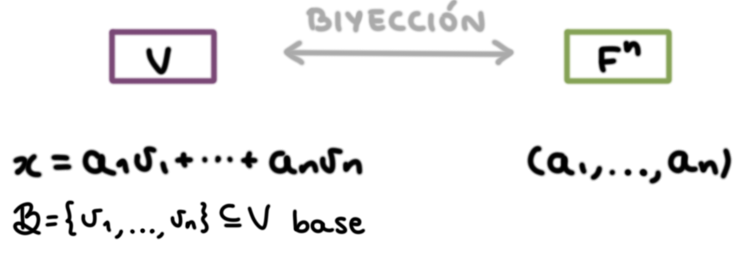
\includegraphics[scale = 3]{4} 
\end{figure}	

\begin{lema}
	\label{lema: S union x es ld sii x en generado de S}
Sean $S$ un subconjunto l.i. de $V$, $x \in V - S$.
Entonces, $S \cup \{ x \}$ es linealmente dependiente si y sólo
si $x \in \langle S \rangle$.
\end{lema}
\noindent
\textbf{Demostración.}
\begin{itemize}
	\item[$\Rightarrow$)] Suponiendo que $x$ no está en el generado por
	$S$, mostremos que $S \cup \{ x \} $ es l.i. o, equivalentemente,
	que todo subconjunto finito de él lo es. Sea 
	$\{ x_{1}, \ldots , x_{n-1} \} \cup \{ x \}$
	un subconjunto finito de $S \cup \{ x \}$ (¿por qué sólo interesa
	el caso en el que el subconjuto contiene a $x$?). Sean 
	$a_{i}$ escalares tales que 
	\[
	a_{1} x_{1} + \cdots + a_{n-1}x_{n-1} + a_{n}x = \hat{0}.
	\]
	Si $a_{n}$ fuese distinto de cero, despejando tendríamos que
	\[
	x = -\frac{a_{1}}{a_{n}}x_{1} + \cdots + -\frac{a_{n-1}}{a_{n}}x_{n-1}
	\in \langle S \rangle \hspace{0.5cm} \lightning
	\]
	Así, $a_{n} = 0$. Luego,
	\[
	a_{1} x_{1} + \cdots + a_{n-1}x_{n-1} = \hat{0}
	\]
	y, como $S$ es l.i., esto último implica la igualdad a cero 
	de todos los coeficientes.
	\item[$\Leftarrow$)] Puesto que
	\[
	x \in \langle S \rangle = \langle (S \cup \{ x \}) - \{ x \} \rangle,
	\]
	según la proposición \ref{prop: ld equiv fried y hugo},
	$S \cup \{ x \}$ es l.d..
\end{itemize}

\QEDB
\vspace{0.2cm}

\begin{teo}
	\label{teo: extrayendo bases de generadores finitos}
\marginnote{El teorema consiste en extrar bases de conjuntos
generadores finitos.} Si un espacio vectorial $V$ es generado
por un conjunto finito $S_{0}$, entonces un subconjunto de $S_{0}$
es base para $V$.
\end{teo}
\noindent
\textbf{Demostración.}
Si $S_{0} = \emptyset, \{ 0 \}$, entonces $V = \{ 0 \}$, y en ambos
casos puede extrarse del conjunto generador $S_{0}$ al vacío,
que es una base del espacio.

Supongamos ahora que $V \neq \{ 0 \}$ o, equivalentemente, que
$S_{0}$ contiene al menos un vector no cero $x_{1}$. Según el ejercicio
REF, $\{ x_{1} \}$ es linealmente independiente. Continue
escogiendo vectores $x_{2}, \ldots , x_{n} \in S_{0}$
tales que $S = \{ x_{1}, \ldots , x_{n} \}$ sigue siendo 
linealmente independiente y 
\begin{equation}
	\label{eq: 0, 28 ag}
	x \in S_{0} - S \Rightarrow S \cup \{ x \}
	\hspace{0.2cm} \textit{ es l.d.. }
\end{equation}
Según el lema 
\ref{lema: S union x es ld sii x en generado de S}, 
esto puede hacerse escogiendo
$x_{i} \in (V - \langle \{ x_{1}, \ldots , x_{i-1} \}) \cap S_{0}$.
\begin{figure}[H]
	\sidecaption{
	Figura que ilustra el proceso para la colección de cuatro
	vectores de $\IR^{3}$ que se muestra en el diagrama.
	\label{fig: 5}
	}
	\centering
	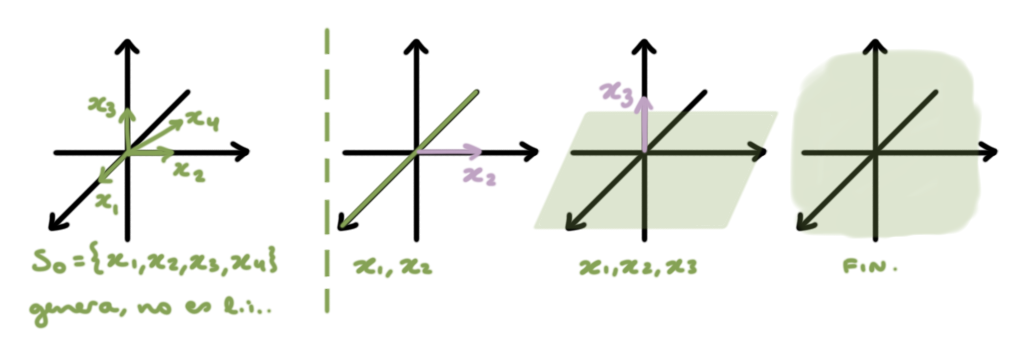
\includegraphics[scale = 2.8]{5} 
\end{figure}	
Como $S$ es finito, este proceso en efecto debe acabar,
es decir, no podemos ampliar indefinidamente a nuestro subconjunto
l.i. de $S_{0}$.

Aformamos que el l.i. $S$ es base del espacio $V$. Para demostrar esto,
bastará ver que $S_{0} \subseteq \langle S \rangle$
pues, en ese caso,
\[
V = \langle S_{0} \rangle \leq \langle \langle S \rangle \rangle
= \langle S \rangle \leq V. 
\]
Sea pues $x \in S_{0}$. Si $x \in S$, claramente 
$x \in \langle S \rangle$. En caso contrario, según 
\ref{eq: 0, 28 ag}, $S \cup \{ x \}$ es l.d., luego,
por el lema \ref{lema: S union x es ld sii x en generado de S},
$x \in \langle S \rangle$.
\QEDB
\vspace{0.2cm}

\begin{cor}
Si un espacio vectorial tiene un subconjunto finito que lo genera,
entonces tiene base (finita).
\end{cor}

La ventaja de la demostración del teorema
\ref{teo: extrayendo bases de generadores finitos}
es que es \textit{constructiva}, es decir, no sólo
muestra la existencia de tales bases, sino que explica
cómo construirlas.

Nota que hasta el momento no hemos dicho nada sobre la existencia
de bases en un espacio vectorial; nos vamos a limitar en esta
sección a hacer inferencias sobre espacios vectoriales que,
por hipótesis, tengan bases. 

\begin{teo}
	\label{teo: un li se completa a generador mediante una base}
\begin{marginfigure}
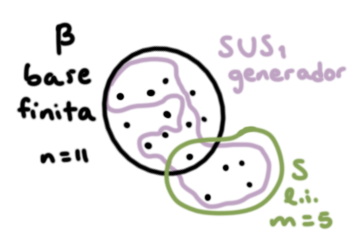
\includegraphics[scale= 3]{7} 
\end{marginfigure}
Sean $V$ un $F-$espacio vectorial, $\beta$ una base $V$ con $n$
elementos, $n \in \IN$. Sea
$S = \{ y_{1}, \ldots , y_{m} \}$ un subconjunto linealmente independiente
con $m \leq n$. Entonces, existe $S_{1}$ subconjunto de $\beta$
con $n-m$ elementos tal que $\langle S \cup S_{1} \rangle = V$.
\end{teo}
\noindent
\textbf{Demostración.}
Vamos a proceder por inducción sobre $m \leq n$.

\begin{figure}[H]
\centering\captionsetup{format = hang}
	\begin{measuredfigure}
		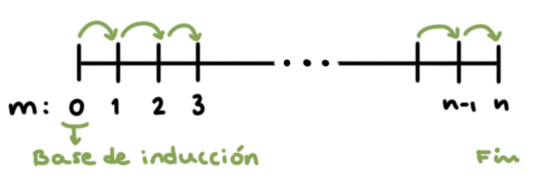
\includegraphics[scale=3]{6} 
 	\end{measuredfigure}
 \end{figure}
\begin{itemize}
\item \textit{Base de inducción:} si $m = 0$, o sea, si $S = \emptyset$,
entonces $S_{1} = \beta$ funciona.
\item \textit{Paso inductivo:} supongamos el teorema cierto para 
$m < n$ y demostremos que el teorema también se cumple para
$m+1$. Sea pues $S = \{ y_{1}, \ldots , y_{m}, y_{m+1} \}$
un subconjunto l.i. de $m+1$ elementos. 
\begin{marginfigure}
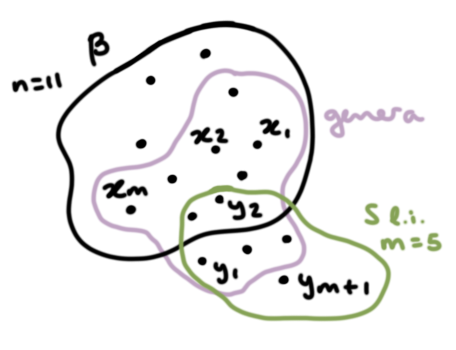
\includegraphics[scale=2.3]{8} 
\end{marginfigure}
Como $\{ y_{1}, \ldots y_{m} \}$ es un l.i. de $m$ elementos, por
hipótesis de inducción existe 
$\{ x_{1}, \ldots , x_{n-m} \} \subseteq \beta$ tal que 
\begin{equation}
	\label{eq: 0 29 Ag 24}
	\langle \{ y_{1}, \ldots , x_{m} \} \cup
	\{ x_{1}, \ldots , x_{n-m} \} \rangle = V.
\end{equation}
Existen pues escalares $a_{i}, b_{j} \in F$
tales que
\[
y_{m+1} = a_{1}y_{1} + \cdots + a_{m}y_{m} + 
b_{1}x_{1} + \cdots + b_{n-m}x_{n-m}.
\] 
Como $S$ es l.i., $y_{m+1}$ no puede ponerse como combinación
lineal de otros elementos de $S$, luego, al menos
algún $b_{j}$ debe no ser cero; sin pérdida de generalidad,
digamos que $b_{1} \neq 0$. Entonces, podemos despejar a 
$x_{1}$ de la ecuación anterior y llegar a que 
\[
x_{1} \in \langle \{ y_{1}, \ldots , y_{m+1} \} \cup
\{ x_{2}, \ldots , x_{n-m} \} \rangle;
\]
de esto se sigue que 
\begin{marginfigure}
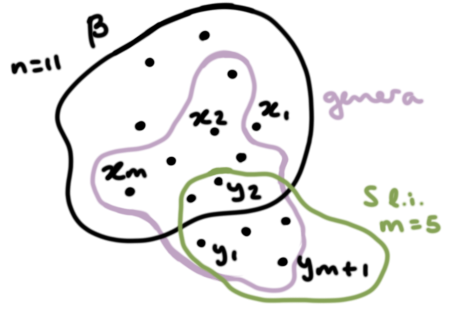
\includegraphics[scale=2.3]{9} 
\end{marginfigure}
\[
\{ y_{1}, \ldots , y_{m}, x_{1}, x_{2}, \ldots , x_{n-m} \}
\subseteq 
\langle
y_{1}, \ldots , y_{m}, y_{m+1}, x_{2}, \ldots, x_{n-m}
\rangle.
\]
Tomando generados a ambos lados de la igualdad y usando 
\eqref{eq: 0 29 Ag 24}, llegamos a que 
el subconjunto $\{x_{2}, \ldots , x_{n-m} \}$ de
$n-(m+1)$ elementos de $\beta$ es tal que 
\[
\langle
\{ y_{1}, \ldots , y_{m+1} \} \cup
\{ x_{2}, \ldots , x_{n-m} \}
\rangle = V.
\]
\end{itemize}
\QEDB
\vspace{0.2cm}

\begin{cor}
	\label{cor: li con n element es base}
Sea $V$ un $F-$espacio vectorial que tiene una base
$\beta$ con $n$ elementos. Entonces, cualquier subconjunto
l.i. de $V$ con $n$ elemenos es base de $V$. 
\end{cor}
\noindent
\textbf{Demostración.}
Según el teorema 
\ref{teo: un li se completa a generador mediante una base},
si $S$ es un tal subconjunto l.i., entonces existe $S_{1} \subseteq \beta$
tal que $S \cup S_{1}$ genera a $V$ y $S_{1}$ tiene
$n-n=0$ elementos; entonces, tal $S_{1}$ debe ser el vacío,
y $S = S \cup \emptyset$, además de ser l.i., genera a $V$,
luego, es base del espacio.

\QEDB
\vspace{0.2cm}

\begin{ejem}
En los ejercicios mostraste que $\IR^{3}$ tiene a 
$\{ (1, 0, 0), (0, 1, 0), (0, 0, 1) \}$ como base. Sean
los vectores 
$x_{1} = (1, -3, 2)$,
$x_{2} = (4, 1, 0)$ y $x_{3} = (0, 2, -1)$. Es fácil ver que
estos son linealmente independientes. Según el corolario
\ref{cor: li con n element es base}, esto implica que
ellos conforman una base para $\IR^{3}$.
\end{ejem}

\marginnote{Este Corolario nos indica que la cardinalidad de una
base finita de $V$ acota la cardinalidad de los subconjuntos
l.i. del espacio.}
\begin{cor}
	\label{cor: cardinalidad de bases limita la de los li}
Sea $V$ un $F-$espacio vectorial. Si existe $\beta$ base de
$V$ con $n$ elementos, entonces cualquier subconjunto de $V$
con más de $n$ elementos es l.d..
\end{cor}
\noindent
\textbf{Demostración.}
Sea $S \subseteq V$ con $|S| > n$. Supongamos que $S$ es l.i..
Si $S_{1}$ es un subconjunto de $S$ con al menos $n$ elementos, 
entonces al igual que $S$ es l.i., luego, por el corolario 
\ref{cor: li con n element es base} es una base del espacio,
entonces,  $\langle S_{1} \rangle = V$.
Si $x \in S - S_{1}$, como $x \in V = \langle S_{1} \rangle$,
por el lema 
\ref{lema: S union x es ld sii x en generado de S},
$S_{1} \cup \{ x \} \subseteq S$ es l.d., luego,
$S$ es l.d.  $\lightning$

\QEDB
\vspace{0.2cm}

\begin{cor}
Sea $V$ un $F-$espacio vectorial. Si existe 
$\beta \subseteq V$ base de $n$ elementos, entonces
cualquier otra base de $V$ tendrá $n$ elementos.
\end{cor}
\noindent
\textbf{Demostración.}
Sea $\gamma \subseteq V$ otra base de $V$.
Como $\gamma$ (respectivamente, $\beta$) es linealmente independiente
y $\beta$ (respectivamente, $\gamma$) es base del espacio,
por el corolario 
\ref{cor: cardinalidad de bases limita la de los li}
$|\gamma| \leq |\beta|$ (respectivamente, 
$|\beta| \leq |\gamma|$).

\QEDB
\vspace{0.2cm}

Este último resultado nos permite introducir la noción 
de dimensión.

\begin{defi}
Un espacio vectorial se dice \textbf{finito dimensional}
si tiene una base que consta de un número finito de elementos.
El único número de elementos en cada base del espacio se llama
la \textbf{dimensión de $V$}, y se denotará por
$dim(V)$. Todo espacio vectorial que no sea finito dimensional
será llamado \textbf{infinito dimensional}.
\end{defi}

Nota que hasta el momento hemos encontrado resultados válidos
para cuando el espacio vectorial tiene una base finita; aunque 
con lo visto hasta ahora no podemos asegurar que cualquier
espacio vectorial tiene base, esto es cierto y puede
demostrarse usando el Lema de Zorn. Puedes consultar los
detalles en Friedberg, sección 1.7.
En la práctica, casi siempre se usarán espacios de dimensión
finita (de hecho, algún $\IR^{n}$).


\begin{ejem}
Demuestre las siguientes afirmaciones:
\begin{itemize}
	\item El espacio vectorial $\{ 0 \}$ tiene dimensión cero.
	\item El espacio vectorial $F^{n}$ tiene dimensión $n$.
	\item El espacio vectorial $M_{m \times n} (F)$ tiene dimensión
	$m \times n$.
	\item El espacio vectorial $P_{n}(F)$ tiene dimensión
	$n+1$.
	\item El espacio vectorial $P(F)$ es infinito dimensional.
\end{itemize}
\end{ejem}


\begin{ejem}
Ilustramos a continuación el que la dimensión de un
$F-$espacio vectorial $V$ depende no solo del grupo abeliano $V$,
sino también del campo $F$.
\begin{itemize}
	\item El $\IC-$ espacio vectorial $\IC$ tiene dimensión $1$.
	En efecto, $\{ 1 \}$ es base para él, pues
	\begin{itemize}
		\item el singulete $\{ 1 \}$ es l.i., y,
		\item dado $z \in \IC$, $z = 1 \cdot z \in \langle \{ 1 \} \rangle$,
		luego, $\langle \{ 1 \} = \IC$.
	\end{itemize}
	\item El $\IR-$espacio vectorial $\IC$ tiene dimensión $2$,
	pues una base de este espacio es $\{ 1, i \}$;
	\begin{itemize}
		\item Dado $z = a + b i \in \IC$ (donde $a, b \in \IR$),
		$z = a \cdot 1 + b \cdot i \in \langle \{ 1, i \} \rangle$, y
		\item no existe $a \in \IR$ tal que $a \cdot 1 = i$, luego,
		$i$ no es múltiplo escalar de $1$, por lo que 
		$\{ 1, i \}$ es l.i..
	\end{itemize}
\end{itemize}
\end{ejem}

\begin{cor}
	\label{cor: generador de n elementos es base en un n dim}
Sea $V$ un $F-$espacio vectorial de dimensión $n$. Si
$S \subseteq V$ genera a $V$ y tiene a lo más $n$ elementos, entonces $S$
es base de $V$ (luego, $|S| = n$).
\end{cor}
\noindent
\textbf{Demostración.}
Por el teorema 
\ref{teo: extrayendo bases de generadores finitos}, 
sabemos que existe $S_{1} \subseteq S$ base de $V$.
Entonces, como $V$ es $n-$dimensional,
$|S_{1}| = n$; entonces, $|S| \leq n$ y $S$ tiene 
un subconjunto $S_{1}$ de $n$ elementos, luego $S$ tiene $n$
elementos y coincide con $S_{1}$, 
por lo tanto, es base de $V$.
\QEDB
\vspace{0.2cm}

\begin{figure}[H]
	\sidecaption{
	Según lo estudiado ahora, la cardinalidad de un 
	subconjunto de un espacio vectorial $n-$dimensional
	nos indica si puede o no ser l.i. o generador.
	}
	\centering
	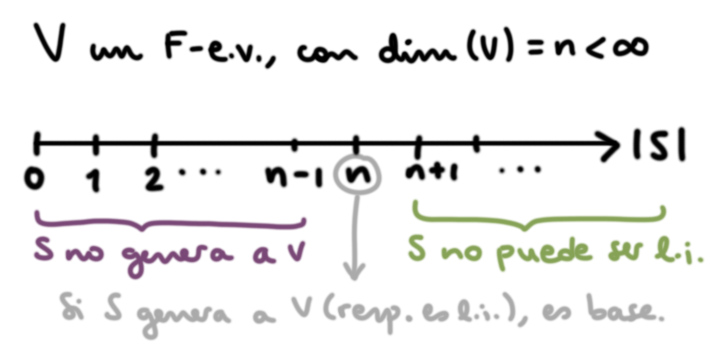
\includegraphics[scale = 3]{10} 
\end{figure}	

\begin{cor}
	\label{cor: extendiendo l.i. a base finita}
\marginnote{Este corolario nos explica cómo extender l.i.'s a 
bases finitas.}
Sea $\beta$ una base de un espacio vectorial $V$ de dimensión
$n$. Sea $S \subseteq V$ linealmente independiente. Existe
$S_{1} \subseteq \beta$ tal que $S \cup S_{1}$ es base de $V$.
\end{cor}
\noindent
\textbf{Demostración.}
Por el corolario \ref{cor: cardinalidad de bases limita la de los li},
$m := |S| \leq n$, entonces, por el teorema 
\ref{teo: un li se completa a generador mediante una base},
existe $S_{1} \subseteq \beta$ con 
$|S_{1}| = n-m$ tal que $S \cup S_{1}$ genera a $V$.
Claro que $|S \cup S_{1}| \leq n$; así, por el corolario 
\ref{cor: generador de n elementos es base en un n dim}, 
$S \cup S_{1}$ es base de $V$.
\QEDB
\vspace{0.2cm}

Resumimos lo deducido hasta ahora:
\begin{itemize}
	\item Una base de un espacio vectorial es un subconjunto de este
	que lo genera y es linealmente independiente.
	\item Si $V$ tiene una base finita, entonces cualquier base de $V$
	tiene el mismo número de vectores. A este número $n$ se le llama la 
	dimensión de $V$.
	\begin{marginfigure}
		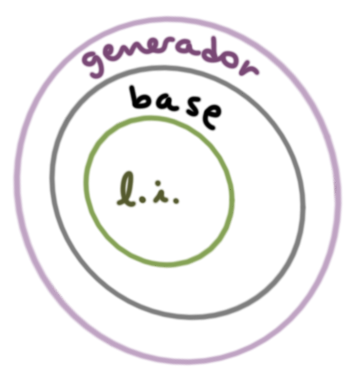
\includegraphics[scale= 2.5]{11}
	\end{marginfigure}
	\item En este caso, todo subconjunto linealmente independiente
	o generador de $n$ elementos es base del espacio,
	\item todo subconjunto l.i. contiene a lo más $n$
	vectores (c.f. corolario
	\ref{cor: cardinalidad de bases limita la de los li}),
	y en caso de tener menos de $n$ vectores (i.e. en caso de no ser base)
	puede completarse a una base
	del espacio (c.f. corolario 
	\ref{cor: extendiendo l.i. a base finita}).
	\item Recíprocamente, si $dim(V) = n$, entonces todo subconjunto
	generador contiene por lo menos $n$ elementos
	y de él se puede extraer una base de $V$ eliminando vectores
	que hagan al generador redundante (recuerda este proceso explicado
	en la demostración del teorema 
	\ref{teo: extrayendo bases de generadores finitos}).

\end{itemize}

\hlpink{Agregar el proceso para extender un l.i. a una base de un
espacio finito dimensional con la ayuda del lema}
\ref{lema: S union x es ld sii x en generado de S}. Poner el ejemplo
práctico en $M_{2 \times 2}(\IR)$.

\section{Caso práctico: Interpolación con polinomios de Lagrange}


La situación es la siguiente: se tiene un conjunto de $n+1$ datos
\marginnote{Interpolación: 
obtención de nuevos puntos partiendo del conocimiento de un conjunto de puntos.}
\[
\{ (c_{0}, b_{0}), (c_{1}, b_{1}), \ldots , (c_{n}, b_{n}) \},
\]
con $c_{i} \neq c_{j}$ si $i \neq j$, y se requiere
hacer una interpolación de estos con un polinomio
del menor grado posible. 
\begin{itemize}
	\item Nos gustaría usar un polinomio, pues es una función
	con la que es muy fácil trabajar, tanto teórica
	como prácticamente.
	\item Además, no queremos que el grado sea alto 
	(relativo a la cantidad de datos) para evitar situaciones
	como las de la figura: el aumentar el grado del polinomio
	aumenta el número de ceros de este, luego, la cantidad de
	oscilaciones, por lo que usar un grado demasiado alto hace
	que, a pesar de que el polinomio coincida con los puntos
	$b_{i}$ en los valores $c_{i}$, no modele bien su patrón
	de comportamiento.
\end{itemize}

\begin{marginfigure}
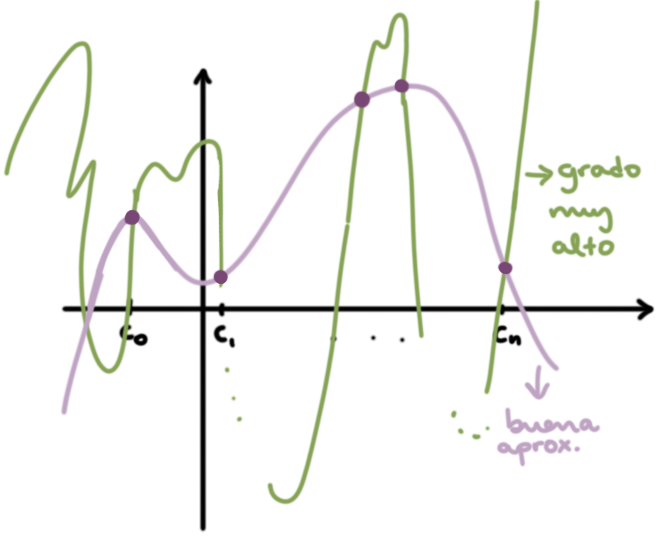
\includegraphics[scale= 1.8]{12} 
\end{marginfigure}

Para $0 \leq i \leq n$, definamos
\begin{equation}
	\label{eq: defi pol lagrange}
	f_{i}(x) := \frac{
	(x-c_{0}) (x-c_{1}) \cdots (x-c_{i-1})
	(x-c_{i+1}) \cdots (x-c_{n})
	}{(c_{i} - c_{0}) (c_{i}-c_{1}) \cdots
	(c_{i}-c_{i-1})(c_{i}-c_{i+1}) \cdots (c_{i}-c_{n}) }
	= \prod_{\substack{j=0 \\ j \neq i}}^{n} \frac{x-c_{j}}{c_{i}-c_{j}}.
\end{equation}
\marginnote{La condición \ref{eq: propiedad pol lagrange} es la que define
a los polinomios de Lagrange.}
A estos $n+1$ polinomios se les llama los
\textbf{polinomios de Lagrange asociados a $c_{0}, c_{1}, \ldots , c_{n}$}.
Por supuesto que
\begin{equation}
	\label{eq: propiedad pol lagrange}
	f_{i}(c_{j}) 
	= \begin{cases}
	0 & \textit{ si } j \neq i, \\
	1 & \textit{ si } j = i.
	\end{cases}
\end{equation}

\begin{figure}[H]
	\sidecaption{
	Polinomios de Lagrange asociados a la malla 
	$[-3, 0.8,  5, 9]$.
	}
	\centering
	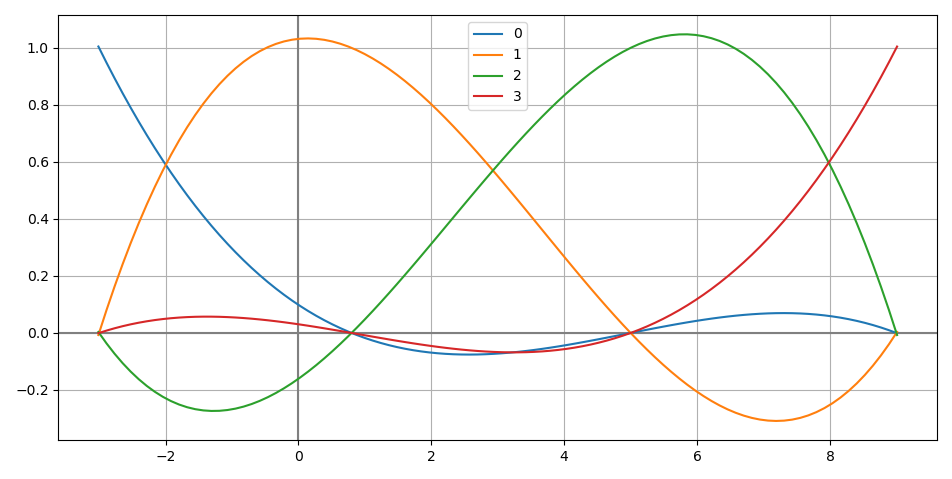
\includegraphics[scale = 0.5]{15} 
\end{figure}	



\begin{prop}
Sean $c_{0} < c_{1} < \cdots < c_{n}$ números reales. Si
$\beta = \{ f_{0}, \ldots, f_{n} \}$ es el conjunto de los
polinomios de Lagrange 
\eqref{eq: defi pol lagrange} asociados a estos números,
entonces $\beta$ es una base del $F$ espacio vectorial
$P_{n}(F)$.
\end{prop}
\noindent
\textbf{Demostración.}
Si demostramos que el conjunto de $n+1$ vectores 
$\beta$ es l.i. podremos concluir que es base de
$P_{n}(F)$ (¿por qué?).
Sean $a_{0}, a_{1}, \ldots, a_{n} \in F$ tales que
$a_{0}f_{0} + \cdots + a_{n}f_{n}$ es el polinomio ero.
Entonces, para toda $0 \leq j \leq n$,
usando la propiedad \eqref{eq: propiedad pol lagrange}
se tiene que 
\begin{align*}
0 = \hat{0}(c_{j}) = &
(a_{0}f_{0} + a_{1}f_{1} + \cdots + a_{n}f_{n})(c_{j}) \\
= & \sum_{i=1}^{n} a_{i}f_{i}(c_{j}) = a_{j} \cdot 1 = a_{j}.
\end{align*}

\QEDB
\vspace{0.2cm}


Así, dado $g \in P_{n}(F)$ cualquiera, existen únicos
$b_{i} \in F$ tales que $g = \sum_{i = 0}^{n}b_{i}f_{i}$;
de hecho, la propiedad \eqref{eq: propiedad pol lagrange}
nos permite dar explícitamente a tales coeficientes $b_{i}$;
para toda $0 \leq j \leq n$,
\[
g(c_{j}) = \left( \sum_{i = 0}^{n}b_{i}f_{i} \right)(c_{j})
= b_{j}.
\]
Así,
\begin{equation}
	\label{eq: g como comb lineal de los de lagrange}
	g = \sum_{i=0}^{n}g(c_{i})f_{i}.
	\hspace{0.2cm} \textit{(Ecuación de interpolación de Lagrange)}
\end{equation}


Regresando a la situación planteada al inicio,
dada la colección de datos 
$$\{ (c_{0}, b_{0}), (c_{1}, b_{1}), \ldots , (c_{n}, b_{n}) \},$$
el único polinomio $g$ de grado a lo más $n$ tal que
$g(c_{i}) = b_{i}$ para toda $i$ es 
\eqref{eq: g como comb lineal de los de lagrange}.

\begin{figure}[H]
	\sidecaption{
	Polinomio de interpolación de Lagrange para los datos
	$(-3,-1), (-2, 4), (-1, 2), (0, 0.8),$ 
	$(2, -0.5), (3, 0.6), (4, 1)$, 
	$(5, 3), (5.5, 3.5)$.
	\label{fig: interp}
	}
	\centering
	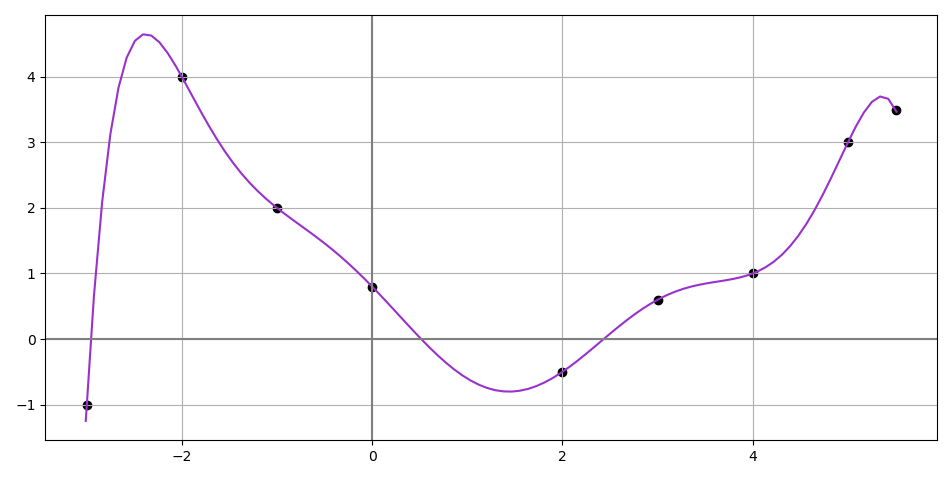
\includegraphics[scale = 0.5 ]{14} 
\end{figure}	




\section{Algunos resultados de dimensión}

\begin{teo}
	\label{teo: la dim de subespacios es menor o igual a la del espacio}
Sea $V$ un $F-$espacio vectorial de dimensión $n$.
Todo subespacio de $V$ será también finito dimensional, y
si dimensión será menor o igual a $n$; si es igual a $n$,
entonces coincide con todo el espacio $V$.
\end{teo}
\noindent
\textbf{Demostración.}
Sea $W \leq V$.
Si $W = \{ 0 \}$, entonces $dim(W) = 0 \leq n$. Supongamos ahora
que W tiene al menos un elemento no cero $x_{1}$.
El singulete
$\{ x_{1} \}$ es entonces l.i.
(c.f. proposición \ref{prop: singulete x l.i. sii x no cero}).
Podemos continuar de esta forma tomando elementos
$x_{1}, \ldots, x_{k}$ de $W$
tales que $\{ x_{1}, \ldots , x_{k} \}$ es l.i.
pero, adjuntando otro vector de $W$, se pierde la independencia
lineal (esto porque en $V$ no puede haber subconjuntos linealmente
independientes de más de elementos, luego, de hecho
ocurre $k \leq n$).
Según el lema 
\ref{lema: S union x es ld sii x en generado de S}, esto implica
que
\[
\forall x \in W - \{ x_{1}, \ldots , x_{k} \}:
\hspace{0.2cm} x \in \langle \{ x_{1}, \ldots , x_{k} \} \rangle,
\]
luego, 
\[
W = \langle \{ x_{1}, \ldots , x_{k} \} \rangle.
\]
Así, el l.i. $\{ x_{1}, \ldots , x_{k} \}$
genera a $W$, por lo tanto, es base de $W$.
Entonces, $dim (W) = k \leq n$.

Si ocurriese $dim(W) = n$, entonces una base $\beta$ de $W$
es un subconjunto l.i. de $V$ de $n = dim(V)$ elementos,
por lo tanto, es también una base de $V$
(c.f. corolario \ref{cor: li con n element es base}),
luego,
\[
W = \langle \beta \rangle = V.
\]
\QEDB
\vspace{0.2cm}

\begin{cor}
Si $V$ es finito dimensional, entonces toda base
$\beta$ de un subespacio de $W$ puede extenderse a una base de $V$.
\end{cor}
\noindent
\textbf{Demostración.}
Si $\beta$ es base de $W$, en particular es un subconjunto
l.i. de $V$, luego, según el corolario 
\ref{cor: extendiendo l.i. a base finita}, puede extenderse a una
base de $V$.
\QEDB
\vspace{0.2cm}

\begin{teo}
Si $W_{1}, W_{2}$ son dos subespacios de $V$ finito dimensionales,
entonces $W_{1} + W_{2}$ es también finito dimensional, y 
\[
dim(W_{1} + W_{2}) = dim(W_{1}) + dim(W_{2}) - dim(W_{1} \cap W_{2}).
\]
\end{teo}
\noindent
\textbf{Demostración.}
Note primero que $W_{1} \cap W_{2}$ es subespacio de un espacio
finito dimensional (por ejemplo, de $W_{1}$), luego, es también
finito dimensional. Sea pues
$\beta_{0} = \{ x_{1}, \ldots , x_{k} \}$ base de 
$W_{1} \cap W_{2}$, y sean 
$\beta_{1} = \{ y_{1}, \ldots , y_{r} \}$, 
$\beta_{2} = \{ z_{1}, \ldots , z_{m} \}$
tales que
\[
\beta_{0} \cup \beta_{i} \hspace{0.5cm}
\textit{ es base de } W_{i}, \hspace{0.1cm} i = 1,2.
\] 
\begin{itemize}
	\item Veamos que $\beta_{0} \cup \beta_{1} \cup \beta_{2}$
	es l.i.. Sea escalares $a_{i}$, $b_{j}$ y $c_{l}$ tales que 
	\begin{equation}
		\label{eq: 1, 5 sept 24}
		a_{1}x_{1} + \cdots + a_{k} x_{k} + 
		b_{1}y_{1} + \cdots b_{r}y_{r} +
		c_{1}z_{1} + \cdots + c_{m}z_{m} = \hat{0}.
	\end{equation}
	Definiendo
	\[
	v_{0} = a_{1}x_{1} + \cdots + a_{k} x_{k},
	\hspace{0.1cm}
	v_{1} = b_{1}y_{1} + \cdots b_{r}y_{r},
	\hspace{0.1cm}
	v_{2} = c_{1}z_{1} + \cdots + c_{m}z_{m},
	\]
	la ecuación \eqref{eq: 1, 5 sept 24}
	se reescribe como
	\[
	v_{0} + v_{1} + v_{2} = \hat{0}.
	\]
	Por supuesto que $v_{0} \in W_{1} \cap W_{2}$,
	$v_{1}  \in W_{1}$, $v_{2} \in W_{2}$.
	Despejando a $v_{2}$ de esta última ecuación, se tiene que
	$v_{2} = v_{0} + v_{1} \in W_{1}$, luego,
	$v_{2} \in W_{1} \cap W_{2}$.
	Puesto que $\beta_{0}$ es base de este espacio, existen
	escalares $d_{i}$ tales que 
	\begin{equation}
		\label{eq: 2, 5 sept 24}
		v_{2} = d_{1}x_{1} + \cdots + d_{n} x_{n};
	\end{equation}
	sustituyendo en \eqref{eq: 1, 5 sept 24}, se llega a que
	\[
	(a_{1}+d_{1})x_{1} + \cdots + (a_{k}+d_{k})x_{k} +
	b_{1}y_{1} + \cdots + b_{k}y_{k} = \hat{0};
	\]
	la independencia lineal de $\beta_{0}\cup \beta_{1}$
	implica que todos los escalares de la combinación lineal
	anterior son cero, en particular, que 
	$b_{1} = \cdots = b_{k} = 0$. Sustituyendo esto en 
	\eqref{eq: 1, 5 sept 24}, se tiene que 
	\[
	(a_{1})x_{1} + \cdots + (a_{k})x_{k} +
	c_{1}z_{1} + \cdots + c_{m}z_{m} = \hat{0}.
	\]
	Ahora la independencia lineal de $\beta_{0} \cup \beta_{2}$
	nos permite concluir que también los escalares $a_{i}$ y
	$c_{l}$ son todos cero.
	
	Con esto demostramos la independencia lineal de 
	$\beta_{0} \cup \beta_{1} \cup \beta_{2}$. Nota que esto
	implica que $\beta_{0}$, $\beta_{1}$ y
	$\beta_{2}$ son ajenos dos a dos, luego,
	\begin{equation}
		\label{eq: cardinalidad de base de w1 mas w2}
		|\beta_{0} \cup \beta_{1} \cup \beta_{2}| = k + r + m.
	\end{equation}
	
	\item Mostremos que
	\marginnote{Es fácil comprobar que, para cualesquiera subconjuntos
	$A, B \subseteq V$, 
	\[
	\langle A \cup B \rangle = \langle A \rangle + 
	\langle B \rangle.
	\]}	
	 $\beta_{0} \cup \beta_{1} \cup \beta_{2}$
	genera a $W_{1} + W_{2}$;
	\begin{align*}
	\langle \beta_{0} \cup \beta_{1} \cup \beta_{2} \rangle
	= & \langle
	( \beta_{0} \cup \beta_{1} ) \cup 
	( \beta_{0} \cup \beta_{2} )
	\rangle \\
	= & \langle  \beta_{0} \cup \beta_{1}  \rangle + 
	\langle  \beta_{0} \cup \beta_{2} \rangle \\
	= & W_{1} + W_{2}. 
	\end{align*}
	
	Hemos demostrado así que 
	$\beta_{0} \cup \beta_{1} \cup \beta_{2}$
	es base de $W_{1} + W_{2}$; de esto y 
	\eqref{eq: cardinalidad de base de w1 mas w2}
	se concluye que 
	\begin{align*}
	dim(W_{1} + W_{1}) = k + r + m = &
	(k+r) + (k+m) - k \\
	= & dim(W_{1}) + dim(W_{2}) - dim(W_{1} \cap W_{2}).
	\end{align*}
\end{itemize}
\QEDB
\vspace{0.2cm}

De este teorema y de la proposición 
\ref{prop: suma directa sii interseccion cero}
se sigue el siguiente

\begin{cor}
Si $W_{1}$ y $W_{2}$ son subespacios de $V$ finito dimensionales,
entonces la suma $W_{1} + W_{2}$ es directa si y sólo si 
\[
dim(W_{1} + W_{2}) = dim(W_{1}) + dim(W_{2}).
\]
\end{cor}


\begin{ejem}
Si $U, V$ son dos subespacios de $\IR^{9}$ ambos de dimensión $5$,
entonces su suma no puede ser directa, pues
\[
9 \geq dim(U + V) = dim(U) + dim(V) - dim(U \cap V) = 10 - dim(U \cap V),
\]
luego, $dim(U \cap V) \geq 1$, por lo que no puede ocurrir
$U \cap V = \{ 0 \}$.
\end{ejem}

\begin{ejem}
Considere al $\IR$ espacio vectorial $P_{4}(\IR)$ de los polinomios
con coeficientes reales y grado no mayor a cuatro.
Sea
\[
U = \{ f \in P_{4}(\IR)  | \hspace{0.2cm} f(6) = 0 \}
\]
el conjunto de los polinomios de grado a lo más cuatro que tienen al
$6$ como raíz. Claro que $U$ es un subespacio
(propia) de $P_{4}(\IR)$,
pues
\begin{itemize}
	\item El polinomio cero tiene a $6$ como raíz,
	\item Si $f, g \in U$ y $a \in \IR$, entonces $6$ es raíz del polinomio
	$af + g$, pues $(af+g)(6) = a \cdot f(6) + g(6) = a \cdot 0 + 0 = 0$.
\end{itemize}
Según el teorema \ref{teo: la dim de subespacios es menor o igual a la del espacio},
$0 \leq dim(U) \leq 4$ (pues $dim(P_{4}) = 5$).
Observe que los cuatro polinomios
\[
f_{i}(x) := (x-6)^{i}, \hspace{0.2cm}
1 \leq i \leq 4
\]
son todos elementos de $U$, y además son linealmente independientes
(sus grados son todos distintos entre sí), luego,
ellos conforman una base para el espacio, y $dim(U) = 4$.

\begin{marginfigure}
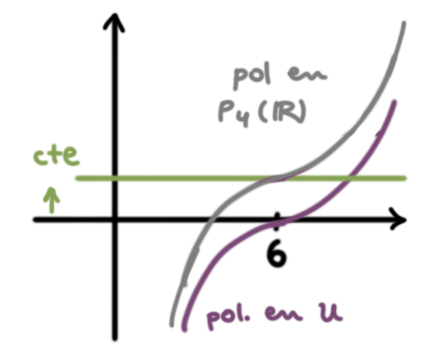
\includegraphics[scale=2]{13} 
		\caption{Todo polinomio en $P_{4}(\IR)$ se
expresa de forma única como la suma de un polinomio en $U$ y 
uno constante.}
\end{marginfigure}

Una base de $P_{4}(\IR)$ que contiene a esta base de $U$ es
\[
\beta = \{ 1, f_{1}, f_{2}, f_{3}, f_{4} \}.
\]
Nota que el subespacio
\[
W = \{ f \in P_{4}(\IR)  | \hspace{0.2cm} f \textit{ es un
polinomio constante o el polinomio cero} \}
\]
es tal que $P_{4}(\IR) = U \oplus W$, pues
$U \cap W = \{ 0 \}$ - el único elemento de $W$ que tiene
a $6$ como raíz es el polinomio cero (de hecho, todo número
real es raíz del polinomio cero, no hay nada especial en el número
$6$ tomado para este ejemplo).
\end{ejem}

Terminemos con unos comentarios más sobre el concepto de dimensión:
es muy importante no confundir la noción de dimensión con
la de cardinalidad: por ejemplo, en $\IR^{3}$, 
\begin{itemize}
	\item toda recta que pasa por el origen es un subespacio
	de dimensión uno, y su cardinalidad $|\IR|$, 
	\item todo plano que pasa por el origen es un subespacio
	de dimensión dos, y su cardinalidad es $|\IR \times \IR| = |\IR|$.
\end{itemize}
Nótese que la dimensión parece ser un mejor indicador del
``tamaño'' de un subespacio, no la cardinalidad de este. 
\newpage










































\section{Ejercicios II}
En lo que sigue, a menos que se indique lo contrario,
$V$ es un $F-$espacio vectorial.
Los ejercicios marcados con el símbolo
$\mathbat$ son obligatorios para los estudiantes de matemáticas,
pero opcionales para los de actuaría.

\begin{ej}
Demuestre que si $f \in P_{n}(f)$ es tal que
$f(c_{j})=0$ para $n+1$ elementos distintos
$c_{0}, \ldots , c_{n}$ del campo $F$, entonces
$f$ es el polinomio cero. 
\textit{Pista:} use polinomios de interpolación de Lagrange
\end{ej}


\begin{ej}
Usando el teorema 
\ref{teo: la dim de subespacios es menor o igual a la del espacio}, 
demuestra que
\begin{itemize}
	\item los únicos subespacios de $\IR^{2}$ son $\{ 0 \}$,
	rectas que pasan por el origen y $\IR^{2}$, y
	\item los únicos subespacios de $\IR^{3}$ son 
	$\{ 0 \}$, rectas y planos que pasan por el origen,
	y $\IR^{3}$.
\end{itemize}
\end{ej}

\newpage
\chapter{Transformaciones lineales}

Ya definimos y estudiamos el concepto de espacio vectorial, dimos
también unos ejemplos que ilustran lo útil que puede ser considerar
espacios vectoriales como marcos teóricos para modelar situaciones
prácticas. Lo que queremos hacer ahora es establecer relaciones entre
espacios vectoriales; más formalmente, queremos 
trabajar con funciones de un espacio vectorial a otro
que preserven la estructura algebráica de estos. Como veremos,
algunos de los conceptos matemáticos más usados pueden
verse de forma natural como transformaciones lineales, por ejemplo,
\begin{itemize}
	\item las operaciones de integración y diferenciación
	del cálculo, o 
	\item las proyecciones, reflexiones y proyecciones de
	la geometría.
\end{itemize}


Explicaremos además cómo codificar la información de una
transformación lineal 
entre espacios vectoriales finito
dimensionales en una matríz (que dependerá de las bases
escogidas para el dominio y codominio), hecho que hará que la teoría
desarrollada sea fácilmente llevada a la práctica - pues estaremos
sustituyendo a las funciones por objetos discretos.

\begin{figure}[H]
	\sidecaption{
	Euclides usa en sus argumentos transformaciones
	lineales como las traslaciones, rotaciones y proyecciones.
	\label{fig: eucl}
	}
	\centering
	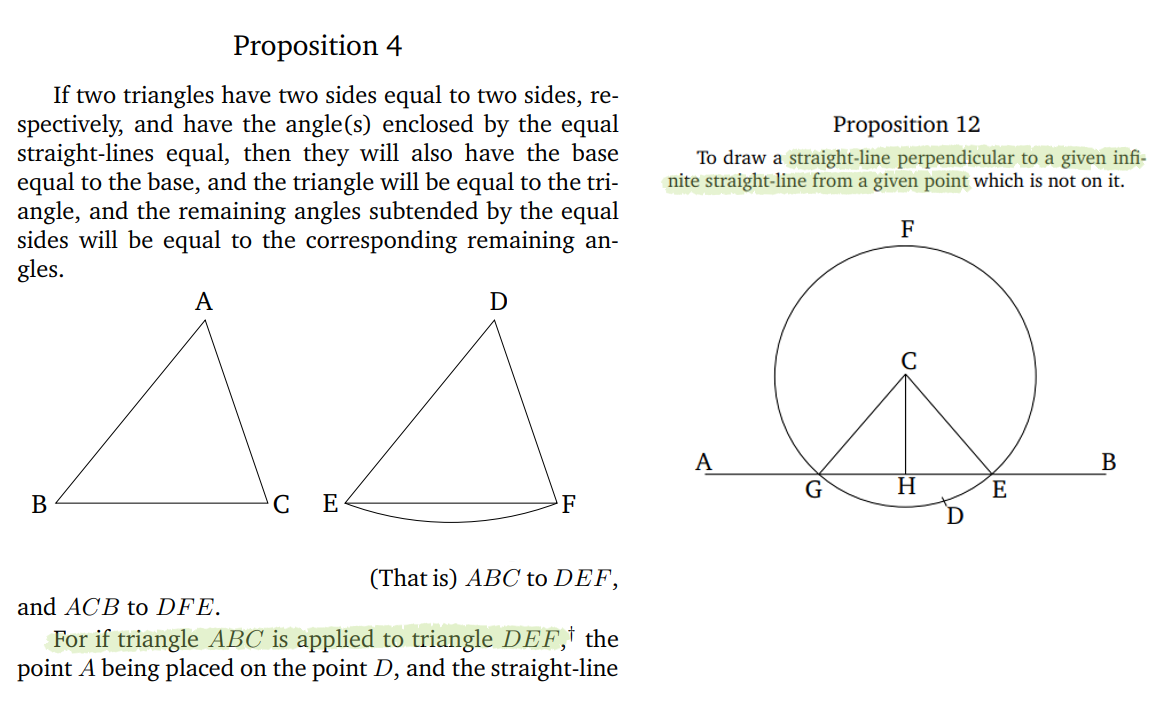
\includegraphics[scale = 2.5]{16} 
\end{figure}	

\section{Transformaciones lineales}

\begin{defi}
Sean $V$, $W$ dos espacios vectoriales sobre un mismo campo $F$.
\marginnote{Nota que $V$ y $W$ deben ser espacios vectoriales sobre un
campo común para que ambos lados de la ecuación
\ref{eq: condicion linealidad} tengan sentido.}
Toda función $T: V \longrightarrow W$ tal que
\begin{equation}
	\label{eq: condicion linealidad}
(\forall x, y \in V) (\forall a \in F): \hspace{0.2cm}
T(ax + y) = a T(x) + T(y)
\end{equation}
será llamada una \textbf{transformación lineal} de $V$ en $W$.
\end{defi}


\begin{obs}
Si $T: V \longrightarrow W$ es una transformación lineal, entonces
\begin{itemize}
	\item $T(0_{V}) = T(0_{W})$, y
	\item Para cualesquiera $n \geq 1$ entero, 
	$a_{1}, \ldots, a_{n} \in F$ y 
	$x_{1}, \ldots , x_{n} \in V$, 
	\[
	T \left( \sum_{i=1}^{n} a_{i}x_{i} \right) = 
	\sum_{i=1}^{n} a_{i}T(x_{i}).
	\]
\end{itemize}
\end{obs}
\noindent
\textbf{Demostración.}
En efecto, tenemos la siguiente ecuación en el grupo abeliano $W$
\[
T(0_{V}) = T(0_{V} + 0_{V}) = T(0_{V}) + T(0_{V}),
\]
luego, $T(0_{V}) = 0_{W}$. El segundo punto se demuestra
por inducción, usando a la condición \eqref{eq: condicion linealidad}
como base de inducción.
\QEDB
\vspace{0.2cm}

\hlgray{Ejercicio:} demuestra que la condición
\ref{eq: condicion linealidad} es equivalente a las siguientes dos
condiciones:
\begin{enumerate}
	\item (\textbf{aditividad})
	Para cualesquiera $x, y \in V: T(x+y) = T(x) + T(y)$,
	\item (\textbf{homogeneidad}) Para cualesquiera $x \in V$, $a \in F$, 
	$T(ax) = a T(x)$.
\end{enumerate}
Estas condiciones dicen que, no importa si primero
se realiza la suma o multiplicación escalar en el espacio $V$
y luego se aplica la transformación lineal, o si primero se llevan
los vectores a $W$ via $T$ y luego se efectua la suma o 
multiplicación escalar en $W$, el resultado es el mismo.

\subsection{Ejemplos de transformaciones lineales}

Tenemos la siguiente lista de ejemplos canónicos de transformaciones
lineales.
\begin{itemize}
	\item Dados $V$ y $W$ $F-$espacios vectoriales,
	las funciones $I_{V}: V \longrightarrow V$
	y $T_{0}: V \longrightarrow W$ definidas como
	\[
	\forall x \in V : \hspace{0.2cm}
	I_{V}(x) = x, \hspace{0.1cm}
	T_{0}(x) = 0_{W}
	\]
	son transformaciones lineales, llamadas respectivamente
	la \textbf{transformación identidad} y 
	la \textbf{transformación cero} en $V$.
	\item La función
	$T: P_{n}(\IR) \longrightarrow P_{n-1}(\IR)$
	definida como
	\[
	\forall f \in P_{n}(\IR) : \hspace{0.2cm}
	T(f) = f'
	\]
	es una transformación lineal.
	\item La función
	$T: \mathcal{C}(\IR) \longrightarrow \IR$
	definida como
	\[
	\forall f \in P_{n}(\IR) : \hspace{0.2cm}
	T(f) = \int_{a}^{b} f(t)dt
	\]
	es una transformación lineal.
	\item Sea $0 \leq \theta < 2 \pi$. La función
	$T_{\theta} : \IR^{2} \longrightarrow \IR^{2}$ definida como 
	\[
	\forall (a, b) \in \IR^{2} : \hspace{0.2cm}
	T_{\theta}(a, b) = (a cos(\theta) - b sen(\theta), 
	a sen(\theta) + b cos(\theta))
	\]
	es una transformación lineal llamada 
	\textbf{rotación de $\theta$ radianes}.
	\item La función $T:\IR^{2} \longrightarrow \IR^{2}$ definida como
	\[
	\forall (a, b) \in \IR^{2} : \hspace{0.2cm}
	T_{\theta}(a, b) = (a, -b)
	\]
	es llamada la \textbf{reflexión sobre el eje $x$}, y es una 
	transformación lineal tal que $T \circ T = T$.
	\item La función $T:\IR^{2} \longrightarrow \IR^{2}$ definida como
	\[
	\forall (a, b) \in \IR^{2} : \hspace{0.2cm}
	T_{\theta}(a, b) = (a, 0)
	\]
	es una transformación lineal, que llamamos \textbf{proyección
	sobre el eje-x}.
\end{itemize}


Profundicemos un poco más la definición de proyección.
Claramente, $W_{1} = \{ (a, 0): \hspace{0.2cm} a \in \IR \}$
y $W_{2} = \{ (0, b): \hspace{0.2cm} b \in \IR \}$
son subespacios de $\IR^{2}$ tales que 
$\IR^{2} = W_{1} \oplus W_{2}$. Se definió arriba a la proyección
sobre el eje-x a la función que, a cada $v \in \IR^{2}$, le 
asigna su sumando correspondiente al espacio $W_{1}$.
Definamos en general el término proyección.
\begin{defi}
	\label{def: proyeccion}
Sea $V$ un $F-$espacio vectorial, $W_{1} \leq V$.
Si $W_{2} \leq V$ es tal que $W_{1} \oplus W_{2} = V$, 
la función $T: V \longrightarrow V$ definida como
\begin{equation}
	\label{eq: proyeccion sobre W1}
	T(x) = x_{1}, \hspace{0.4cm}
x = x_{1} + x_{2}, \hspace{0.2cm}
x_{1} \in W_{1}, x_{2} \in W_{2}
\end{equation}
es llamada
una \textbf{proyección sobre $W_{1}$}.
\end{defi}

\begin{nota}
	Si $U, V, W$ son subespacios de
	un $F-$espacio vectorial, la igualdad $U \oplus V = U \oplus W$ 
	\textbf{no implica} la igualdad $V = W$.
	
	Por ejemplo, considérese a los subespacios de $\IR^{2}$
	\[
	U = span(\{(1, 0)\}), \hspace{0.2cm} \textit{ eje x},
	\]
	\[
	V = span(\{(0, 1)\}), \hspace{0.2cm} \textit{ eje y},
	\]
	\[
	W = span(\{(1, 1)\}), \hspace{0.2cm} \textit{ gráfica de la recta $y = x$}.
	\]
	Puesto que $U \cap V = \{0\} = U \cap W$, la suma de $U$ con 
	$V$ y de $U$ con $W$ es directa (c.f. Proposición
	\ref{prop: suma directa sii interseccion cero}), y de hecho es todo el espacio:
	\[
	U \oplus V = \IR^{2} = U \oplus W.
	\]
	Sin embargo, claro que $V \neq W$. 
	Observa que 
	\[
	\forall (x, y) \in \IR^{2}: \hspace{0.2cm}
	x (1, 0) + y (0, 1) = (x, y) = (x-y) (1, 0) + y(1, 1).
	\]
	$\diamond$
\end{nota}


Observe que, como se usa una suma directa para
definir una proyección, la expresión
\eqref{eq: proyeccion sobre W1}
en efecto define una función $T$, de hecho lineal, pues,
si $x = x_{1} + x_{2}$, $y = y_{1} + y_{2}$ y $a \in F$,
entonces,
\[
T(ax + y) = 
T((ax_{1} + y_{1}) + (x_{2}+y_{2}))
= ax_{1} + x_{2} =
a T(x_{1}) + T(x_{2}).
\] 
Note que $W_{1} = \{ x \in V  | \hspace{0.2cm} T(x) = x \}$,
es decir, el conjunto de puntos fijos de una proyección
en $W_{1}$ coincide con $W_{1}$. 
En la Definición \ref{def: proyeccion}
hablamos de ``una'' proyección a $W_{1}$; esto es porque, 
como mostramos a continuación, hay tantas
transformaciones lineales que satisfacen la 
definición de proyección
a $W_{1}$ como subespacios cuya suma directa
con $W_{1}$ es todo el espacio.

\begin{prop}
Sea $W_{1} \leq V$. Si $W_{2}, \tilde{W_{2}}$ son dos
subespacios de $V$ distintos entre si tales que
$V = W_{1} \oplus W_{2} = W_{1} \oplus \tilde{W_{2}}$, entonces
las transformaciones lineales
$T, \tilde{T}: V \longrightarrow V$ definidas como
\[
T(x) = x_{1}, \hspace{0.4cm}
x = x_{1} + x_{2}, \hspace{0.2cm}
x_{1} \in W_{1}, x_{2} \in W_{2}
\]
y 
\[
\tilde{T}(x) = \tilde{x}_{1}, \hspace{0.4cm}
x = \tilde{x}_{1} + 
\tilde{x}_{2}, \hspace{0.2cm}
\tilde{x}_{1} \in W_{1}, 
\tilde{x}_{2} \in \tilde{W_{2}}
\]
son distintas entre si.
\end{prop}
\noindent
\textbf{Demostración.}
Busquemos un punto en el que $T$
y $\tilde{T}$ difieren. Como 
$W_{2} \neq \tilde{W_{2}}$, sin pérdida de generalidad
podemos suponer que existe $y \in \tilde{W_{2}}-W_{2}$.
Se tiene que 
\[
x_{1} + x_{2} = y = 0 + y,
\]
con $x_{1} \in W_{1}$, $x_{2} \in W_{2}$
y $y \in \tilde{W_{2}}$. Note que $x_{1}$ no es
cero, de lo contrario, se tendría
\[
y = x_{2} \in W_{2} \hspace{0.5cm}
\lightning
\]
Así, 
\[
T(y) = x_{1} \neq 0 = \tilde{T}(y).
\]
\QEDB
\vspace{0.2cm}


\begin{figure}[H]
		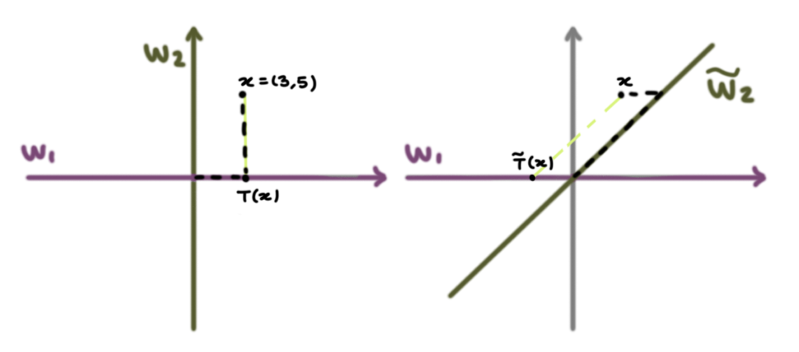
\includegraphics[scale=3.3]{17} 
 \end{figure}

\begin{ejem}
\hlpink{Poner este ejemplo mucho antes.}
Sea $V$ un $F-$espacio vectorial con $dim(V) = n$.
Si $\beta$ es una base de $V$, dividámosla en dos subconjuntos
$\alpha, \gamma$
ajenos cuya unión sea $\beta$. Entonces, $V = 
\langle \alpha \rangle \oplus \langle \gamma \rangle $,
pues 
\begin{itemize}
	\item $V = \langle \alpha \cup \gamma \rangle = 
	\langle \alpha \rangle + \langle \gamma \rangle$,
	y
	\item la suma es directa, pues
	\begin{align*}
	dim(V) = dim(\langle \alpha \rangle + \langle \gamma \rangle) &
	= dim(\langle \alpha \rangle) + 
	dim(\langle \gamma \rangle) - 
	dim(\langle \alpha \rangle \cap \langle \gamma \rangle) \\
	= & dim(V) + 
	dim(\langle \alpha \rangle \cap \langle \gamma \rangle),
	\end{align*}
	luego, $dim(\langle \alpha \rangle \cap \langle \gamma \rangle)
	= 0$, o sea, $\langle \alpha \rangle \cap \langle \gamma \rangle =
	\{ 0 \}$.
\end{itemize}
\end{ejem}
\section{El teorema fundamental de las transformaciones lineales}

La condición \eqref{eq: condicion linealidad} significa que
\marginnote{Recuerda que, si $f: A \longrightarrow B$ es una función cualquiera
y $X \subseteq A$, $Y \subseteq B$, definimos
\[
f(X) := \{ y \in B  | \hspace{0.2cm} \exists x \in X: f(x) = y \},
\]
y
\[
f^{-1}(B) = \{ x \in A  | \hspace{0.2cm} f(x) \in B \}
\]}
la función $T$ preserva la estructura algebráica de $V$. Como
veremos a continuación, toda transformación lineal también
preserva subespacios.
\begin{prop}
Sean $V$ y $W$ $F-$espacios vectoriales,
$T: V \longrightarrow W$ una transformación lineal entre estos.
\begin{itemize}
	\item La imagen de todo subespacio de $V$ bajo $T$ es un 
	subespacio de $W$, es decir,
	\[
	\forall X \subseteq V: \hspace{0.2cm}
	X \leq V \Rightarrow T(X) \leq W.
	\]
	\item La preimagen de todo subespacio de $W$ bajo $T$
	es un subespacio de $V$, es decir, 
	\[
	\forall Y \subseteq W: \hspace{0.2cm}
	Y \leq V \Rightarrow T^{-1}(Y) = 
	\{ x \in V  | \hspace{0.2cm} T(x) \in Y \} \leq V.
	\]
\end{itemize}
\end{prop}
\noindent
\textbf{Demostración.}
En efecto, si $X$ es un subespacio de $V$,
	entonces $0_{V} \in X$, luego, 
	$0_{W} = T(0_{V}) \in T(X)$. Además, si 
	$a$ es un escalar cualquiera y 
	$y_{1}, y_{2} \in T(X)$, entonces existen
	$x_{1}, x_{2} \in V$ tales que 
	$y_{i} = T(x_{i})$, con $i = 1,2$. Así,
	\[
	ay_{1} + y_{2} = a T(x_{1}) + T(x_{2})
	= T(ax_{1} + _{2})
	\]
	es elemento de $T(X)$ pues $X$, al ser subespacio
	de $V$, contiene a $ax + y$.
La demostración del segundo punto es dual.
\QEDB
\vspace{0.2cm}

Vamos ahora a asociar a una transformación
lineal dos espacios vectoriales (uno será un subespacio del
dominio, otro del codominio) de gran importancia.
\begin{defi}
\begin{marginfigure}
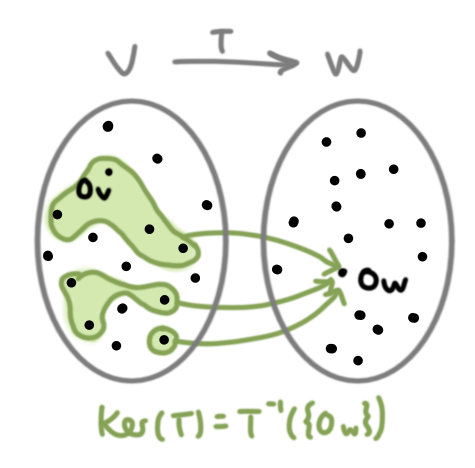
\includegraphics[scale= 2]{kernel} 
		\caption{Etimológicamente, ``kernel'' significa semilla,
		centro, esencia.}
\end{marginfigure}
Sean $V$, $W$ $F-$espacios vectoriales, $T: V \longrightarrow W$
una transformación lineal.  
\begin{itemize}
	\item Se define al \textbf{espacio nulo} de $T$
	o \textbf{kernel} de $T$ como 
	\begin{equation}
		\label{eq: kernel de T}
		Ker(T) := T^{-1}(\{ 0_{W} \}) \leq V.
	\end{equation}
	\item La \textbf{imagen} de $T$
	es \begin{equation}
		\label{eq: rango de T}
		T(V) \leq W.
	\end{equation}
\end{itemize}
\begin{marginfigure}
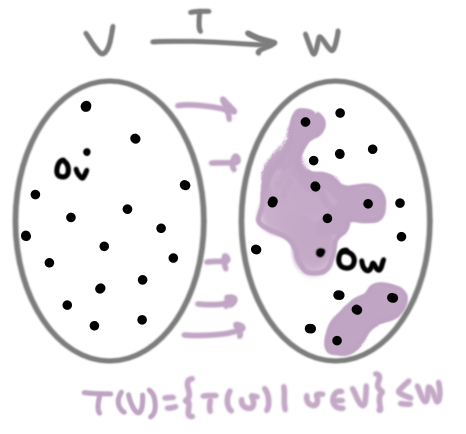
\includegraphics[scale= 2]{imagen} 
\end{marginfigure}
Si $Ker(T)$ es finito dimensional, a su dimensión se le denomina
la \textbf{nulidad de $T$}. Si $T(V)$ es finito dimensional,
su dimensión se conoce como el \textbf{rango de $T$}.
\end{defi}

Observa que el ``tamaño'' del kernel de una transformación lineal
parece ser inversamente proporcional al de la imagen de esta;
en efecto, si muchos vectores pertenecen al kernel, entonces
no habrá muchos vectores en la imagen de $T$ que no sean cero,
lo que achica a $T(V)$. El siguiente teorema, pilar del 
álgebra lineal, da forma a esta intuición.

\begin{teo}
	\label{teo: fundamental de las transf lineales}
\textbf{(fundamental de las transformaciones lineales), 
\textbf{teorema de la dimensión}}
Sean $V$, $W$ $F-$ espacios vectoriales, con $V$
finito dimensional.
Para toda
transformación lineal $T: V \longrightarrow W$,
\begin{equation}
	\label{eq: dim de V es nulidad mas rango}
	dim(V) = dim(Ker(T)) + dim(T(V)),
\end{equation}
es decir, la dimensión del espacio de origen $V$
es igual a la nulidad de $T$ más el rango de $T$.
\end{teo}
\noindent
\textbf{Demostración.}
Como $V$ es finito dimensional, el kernel de $T$ también lo es.
Sea pues $\{ n_{1}, \ldots, n_{k} \}$ una base de $Ker(T)$.
Extendamos este subconjunto l.i. de $V$ a una base de $V$;
sea $\{ v_{1}, \ldots , v_{l} \}$ tal que 
\[
\beta :=
\{ n_{1}, \ldots , n_{k} \} \cup \{ v_{1}, \ldots , v_{l} \}
\]
\marginnote{El Teorema
\ref{teo: fundamental de las transf lineales} es también
conocido como el ``Teorema de la dimensión''.}
es base de $V$. Entonces, $dim(V) = k+l$.
Afirmamos que 
$\{ T(v_{1}), \ldots, T(v_{l}) \}$
es base de la imagen $T(V)$.
\begin{itemize}
	\item Sean $a_{1}, \ldots, a_{l}$ escalares tales que
	\[
	a_{1} T(v_{1}) + \cdots + a_{l} T(v_{l}) = 0_{W}
	\]
	Supongamos que alguno de ellos no es cero; sin pérdida de
	generalidad, digamos que $a_{1} \neq 0$. Por la linealidad
	de $T$, la ecuación anterior se reescribe como
	\[
	T(a_{1}v_{1} + \cdots + a_{l}v_{l}) = 0_{W},
	\]
	es decir,
	\[
	a_{1}v_{1} + \cdots + a_{l}v_{l} \in Ker(T) =
	span(\{ n_{1}, \ldots , n_{k} \}),
	\]
	por lo tanto, 
	\[
	v_{1} \in span(\{ n_{1}, \ldots , n_{k} \}
	\cup \{ v_{2}, \ldots , v_{l} \}).
	\]
	Esto, según el Lema 
	\ref{lema: S union x es ld sii x en generado de S}, contradice
	la independencia lineal de $\beta$.
	\item Claro que $\{ T(v_{1}), \ldots, T(v_{l}) \}$
	genera a $T(V)$ pues, dado $y \in T(V)$, existe 
	$x \in V$ tal que $y = T(x)$. Como $\beta$ es base de $V$,
	existen escalares $a_{i}, b_{j}$ tales que 
	\[
	x = a_{1} n_{1} + \cdots + a_{k} n_{k} + 
	b_{1}v_{1} + \cdots b_{l}v_{l};
	\]
	evaluando ambos lados de la igualdad bajo $T$ y recordando
	que los vectores $n_{i}$ son mapeados al cero (pues 
	son elementos del kernel de $T$), concluimos que
	\[
	y = T(x) = b_{1}T(v_{1}) + \cdots + b_{l}T(v_{l}).
	\]
\end{itemize}
Así, 
\[
dim(V) = k + l = dim(Ker(V)) + dim(T(V)).
\] 
\QEDB
\vspace{0.2cm}

\hlpink{Poner una nota para que ya no confundan el rango de $T$
con el codominio de $T$.}

\begin{cor}
	\label{cor: imagen de base de V bajo lineal genera a W}
Sean $V$ y $W$ son $F-$espacios vectoriales con $V$
finito dimensional, $T: V \longrightarrow W$ lineal.
Para toda $\beta \subseteq V$ base de $V$ se tiene que
$T(\beta)$ genera a $T(V)$.
\end{cor}



\subsection{No ejemplos de transformaciones lineales}

\begin{itemize}
	\item La función $f: \IR \longrightarrow \IR$ definida como
	\[
	f(x) = e^{x}
	\]
	no es lineal, pues $f(0) \neq 0$ (de hecho, la exponencial
	es una función estríctamente positiva).
	\item La función valor absoluto $| \cdot | : \IR \longrightarrow \IR$
	no es lineal. Por ejemplo,
	\[
	|2+(-1)| = |1| = 1 \neq 3 = |2| + |-1|.
	\]
	\item El polinomio $f: \IR \longrightarrow \IR$
	definido como $f(x) = x^{2}$ no es una transformación lineal pues,
	en general, no se cumple que $(x+y)^{2}$ coincida con
	$x^{2} + y^{2}$. De hecho, lo que ocurre es 
	$(x+y)^{2} = x^{2} + 2xy + y^{2}$.
	\item Sea la función $f : \IR^{2} \longrightarrow \IR^{2}$ definida como
	\begin{align*}
	f(x, y )= \begin{cases}
	(2x, 0) & \textit{ si } y = 0 \\
	(x, y) & \textit{ si } y \neq 0.
	\end{cases}
	\end{align*}
	Es fácil comprobar que, a pesar de que $f$ es homogenea, no es
	lineal. Por ejemplo,
	\[
	f((1, 0) + (0, 1)) = f(1, 1) = (1, 1),
	\]
	pero
	\[
	f(1, 0) + f(0, 1) = (2, 0) + (0, 1) = (2, 1).
	\]
	\item La función coseno evaluada en cero vale uno, luego, 
	no es lineal.
	\item Según el Teorema \ref{teo: fundamental de las transf lineales},
	si $T: \IR \longrightarrow \IR$ es lineal, entonces
	\[
	1 = dim(Ker(T)) + dim(T(V)),
	\]
	luego, tenemos dos casos:
	\begin{enumerate}
		\item $dim(T(V)) = 1$, luego, como $T(V)$ es subespacio
		de $\IR$, con $\IR$ uno dimensional, tenemos que 
		$T(V)$ es suprayectiva.
		\item $dim(T(V)) = 0$, es decir,
		$dim(Ker(T)) = 1$. Puesto que $Ker(T) \leq \IR$
		y $dim(\IR) = 1$, se tiene que $Ker(T) = \IR$, luego,
		$T$ es la transformac
		ión lineal cero.
	\end{enumerate}
	Puesto que la función seno 
	\[
	sen(x) : \IR \longrightarrow \IR
	\]
	no es ni la función cero no suprayectiva, no puede ser lineal.
\end{itemize}


\section{Inyectividad y suprayectividad de transformaciones lineales}
Recuerda que, en general, si $f: V \longrightarrow W$ es una
función de un conjunto $V$ a otro conjunto $W$, $f$ se dice
\begin{itemize}
	\item \textbf{inyectiva} si
	\[
	\forall x, y \in V :\hspace{0.2cm}
	T(x) = T(y) \Rightarrow x = y,
	\]
	o, equivalentemente, si las imágenes de puntos
	distintos son distintas
	\item \textbf{suprayectiva} si 
	\[
	(\forall z \in W) \hspace{0.1cm}
	(\exists x \in V): \hspace{0.2cm} T(x) = z.
	\]
\end{itemize}
Resulta que, si $V$ y $W$ son 
$F-$espacios vectoriales y $T: V \longrightarrow W$ es,
no sólo una función, sino una transformación lineal entre ellos,
\marginnote{Veremos que, en el contexto de transformaciones lineales,
los conceptos de inyectividad e independencia
lineal están íntimamente ligados, así como los de 
suprayectividad y generación.}
entonces podemos encontrar equivalencias de ser inyectiva
o suprayectiva usando propiedades del Kernel y la 
preservación de la generación o inyectividad de subconjuntos de $V$.

\begin{prop}
	\label{prop: caracterizacion de inyectividad}
Sean $V$, $W$ dos $F-$espacios vectoriales. Si $T: V \longrightarrow W$
es lineal, las siguientes son equivalentes:
\begin{enumerate}
	\item $T$ es inyectiva
	\item $Ker(T) = \{ 0 \}$
	\item Si $X \subseteq V$ es linealmente independiente,
	entonces $T(X) \subseteq W$ es también linealmente independiente.
\end{enumerate}
\end{prop}
\noindent
\textbf{Demostración.}
\begin{itemize}
 	\item[$1) \Rightarrow 2)$] Si $x \in Ker(T)$ entonces,
 	por definición del kernel, $T(x) = 0$. Además,
 	como $T$ es lineal, también se tiene $T(0) = 0$, luego, como 
 	$T$ es inyectiva, tenemos que $x = 0$. Así, $Ker(T) = \{ 0 \}$.
 	\item[$2) \Rightarrow 1)$] Sean $x, y \in V$ tales que
 	$T(x) = T(y)$. Entonces, por la linealidad de $T$, 
 	$T(x-y) = T(x) - T(y) = 0 $, así, 
 	$x-y \in Ker(T) = \{ 0 \}$, es decir,
 	$x- y = 0$, o sea, $x = y$.
 	\item[$2) \Rightarrow 3)$] Sean $v_{1}, \ldots , v_{n} \in X$
 	cualesquiera; mostremos que $\{ T(v_{1}), \ldots , 
 	T(v_{n}) \}$ es linealmente independiente.
 	\marginnote{En la implicación $2) \Rightarrow 3)$, estamos mostrando
 	que un subconjunto finito arbitrario de $T(X)$ es l.i. suponiendo
 	que $X$ es l.i.. Recuerda que esto es necesario y suficiente para 
 	demostrar la independencia lineal de todo $T(X)$.}
 	Sean $a_{i} \in F$ escalares tales que
 	\[
 	a_{1} T(v_{1}) + \cdots + a_{n} T(v_{n}) = \hat{0}_{W}.
 	\]
 	Por ser $T$ lineal, podemos reescribir el lado izquierdo de la
 	igualdad anterior;
 	\[
 	T(a_{1}v_{1} + \cdots + a_{n}v_{n}) = \hat{0}_{W}.
 	\]
 	Esto muestra que 
 	$a_{1}v_{1} + \cdots + a_{n}v_{n} \in Ker(T) = \{ 0 \}$, luego,
 	\[
 	a_{1}v_{1} + \cdots + a_{n}v_{n} = 0_{V}.
 	\]
 	Como $X$ es l.i., esto implica que todos los escalares
 	$a_{i}$ son cero.
 	\item[$3) \Rightarrow 2)$] Supongamos que existe
 	$x \in Ker(T) - \{ 0 \}$. Como $x$ no es el vector cero, 
 	el singulete $\{ x \}$ es l.i. y, sin embargo, 
 	$\{ T(x) \} = \{ 0_{W} \}$ es l.d.. Esto contradice nuestra
 	hipótesis. 
\end{itemize}

\QEDB
\vspace{0.2cm}

\begin{prop}
\marginnote{Se demuestra que si $f: A \longrightarrow B$ es una función
suprayectiva, entonces, para todo $Y \subseteq B$,
se tiene $f(f^{-1}(Y))= Y$.}
Sean $V$, $W$ dos $F-$espacios vectoriales. Si $T: V \longrightarrow W$
es lineal, las siguientes son equivalentes:
\begin{enumerate}
	\item $T$ es suprayectiva
	\item Si $X \subseteq V$ genera a $V$ entonces $T(X)$
	genera a $W$.
\end{enumerate}
\end{prop}
\noindent
\textbf{Demostración.}
\begin{itemize}
	\item[$1) \Rightarrow 2)$] Sea $X$ un generador de $V$,
	es decir, un subconjunto tal que $span(X) = V$.
	Esto significa que el único subespacio de $V$ que contiene a 
	$X$ es el mismo $V$. Puesto que
	$X \subseteq T^{-1}(span(T(X)))$
	(pues, dado $x \in X$, $T(x) \in T(X) \subseteq 
	span(T(X))$), se tiene entonces
	$T^{-1}( span(T(X)) ) = V$. Evaluando ambos lados
	de la igualdad bajo la función suprayectiva $T$ concluimos que
	\[
	W = T(V) = T(T^{-1}( span(T(X))  )) =  span(T(X)),
	\]
	o sea, que $T(X)$ genera a $W$.
	\item[$2) \Rightarrow 1)$] V trivialmente se genera a sí mismo,
	luego, por hipótesis debe ocurrir que $T(V)$ genere a $W$, o sea,
	que 
	\[
	W = span(T(V)) = T(V),
	\]
	por lo tanto $T$ es suprayectiva.
\end{itemize}

\QEDB
\vspace{0.2cm}

\begin{prop}
Sean $V$ y $W$ dos $F-$espacios vectoriales finito dimensionales.
\begin{itemize}
	\item Si $dim(V) > dim(W)$, entonces no existen transformaciones
	lineales de $V$ en $W$ inyectivas.
	\item Si $dim(V) < dim(W)$, entonces no existen transformaciones
	lineales de $V$ en $W$ suprayectivas.
\end{itemize}
\end{prop}
\noindent
\textbf{Demostración.}
En efecto, 
\begin{itemize}
	\item si existe $T: V \longrightarrow W$ inyectiva, entonces,
	según la proposición \ref{prop: caracterizacion de inyectividad},
	$Ker(T) = \{ 0 \}$, luego, la ecuación
	\eqref{eq: dim de V es nulidad mas rango} se reescribe como
	\[
	dim(V) = dim(T(V)) \leq dim(W).
	\]
	\item Si existe $T: V \longrightarrow W$ suprayectiva,
	entonces $T(V)= W$, luego, 
	\eqref{eq: dim de V es nulidad mas rango} se reescribe como
	\[
	dim(V) = dim(Ker(T)) + dim(W) \geq dim(W).
	\]
\end{itemize}
\QEDB
\vspace{0.2cm}

\section{Isomorfismos}

\begin{defi}
\marginnote{Es decir, una transformación lineal
$T: V \longrightarrow W$ es un isomorfismo si 
$Ker(T) = \{ 0_{V} \}$ y $T(V) = W$.}
Sean $V, W$ dos $F-$espacios vectoriales. Toda transformación
lineal $T: V \longrightarrow W$ que sea biyectiva 
(i.e. inyectiva y suprayectiva) será llamada
un \textbf{isomorfismo}. Si existe un isomorfismo
entre dos espacios vectoriales $V$ y $W$
decimos que $V$ y $W$ son \textbf{isomorfos}.
\end{defi}

Recuerda de tus cursos anteriores que una \textit{función}
$f: A \longrightarrow B$ es biyectiva si y sólo si 
es invertible (i.e. si y sólo si existe una función
$g: B \longrightarrow A $ tal que $f \circ g = Id_{B}$ y
$g \circ f = Id_{A}$). Entonces, una transformación lineal
$T:V \longrightarrow W$ es un isomorfismo si y sólo si 
existe una función $U: W \longrightarrow V$ que sea su inversa.
Claro que tal inversa de existir es única, y se le suele denotar
por $T^{-1}$.
Como establecemos
a continuación, tal función es, al igual que $T$, una transformación lineal.
\begin{prop}
	Si $T: V \longrightarrow W$ es un isomorfismo, entonces
	su función inversa $T^{-1}$ es también un isomorfismo.
\end{prop}
\noindent
\textbf{Demostración.}
Basta probar la linealidad de $T^{-1}$. Sean pues
$y, z \in W$, $\lambda \in F$. Puesto que $T$ es lineal
y $u := T^{-1}(y)$, $v := T^{-1}(z)$ son vectores de $V$,
se tiene que 
\[
T( \lambda u + v) = \lambda T(u) + T(v) = \lambda y +z,
\]
luego,
\[
T^{-1}(\lambda y + z) = \lambda u + v = \lambda T^{-1}(y) + T^{-1}(z).
\]

\QEDB
\vspace{0.2cm}



Mostremos ahora que,
si $V$ es finito dimensional, entonces puede
establecerse un isomorfismo entre $V$
y otro $F-$espacio vectorial $W$ sólo si
$W$ tiene la misma dimensión que $V$.

\begin{prop}
	\label{prop: isomorfo implica misma dimension}
Sea $T: V \longrightarrow W$ lineal, con $V$
de dimensión finita. Si $T$ es un isomorfismo, entonces
$W$ también es finito dimensional y, de hecho,
$dim(W) = dim(V)$.
\end{prop}
\noindent
\textbf{Demostración.}
Digamos que $dim(V)=n$.
Por ser $T$ un isomorfismo, se tiene que
\[
Ker(T) = \{ 0_{V} \} \hspace{0.2cm} \textit{ y }
\hspace{0.2cm} T(V) = W.
\]
Además, como $V$ es finito dimensional, podemos usar el Teorema
\ref{teo: fundamental de las transf lineales}
para deducir que
\begin{align*}
n = dim(V) = & dim(Ker(T)) + dim(T(V)) \\
= & dim(\{ 0_{V} \}) + dim(W) \\
= & 0 + dim(W) = dim(W).
\end{align*} 
\QEDB
\vspace{0.2cm}
 
 
 Mostremos ahora que, cuando se trata con espacios vectoriales finito
 dimensionales, los conceptos de inyectividad, suprayectividad
 y biyectividad en transformaciones lineales son equivalentes.
\begin{teo}
	\label{teo: inyectiva sii supra sii biyect en dim finita}
Sean $V$, $W$ dos $F-$espacios vectoriales, ambos de dimensión
$n$. Entonces, para cualquier transformación lineal
$T: V \longrightarrow W$, son equivalentes
\begin{enumerate}
	\item $T$ es inyectiva
	\item $T$ es suprayectiva
	\item $T$ es biyectiva (i.e. un isomorfismo).
\end{enumerate}
\end{teo}
\noindent
\textbf{Demostración.}
Basta demostrar que $1)$ implica $2)$ y que
$2)$ implica $3)$.
\begin{itemize}
	\item[$1) \Rightarrow 2)$] Si $T$ es inyectiva entonces
	$Ker(T) = \{ 0 \}$, luego, por el Teorema 
	\ref{teo: fundamental de las transf lineales},
	\[
	n = dim(V) = dim(Ker(T)) + dim(T(V)) = 0 + dim(T(V)) =
	dim(T(V)),
	\]
	luego, como $dim(W) = n$ y $T(V) \leq W$ tiene dimensión $n$,
	concluimos que $T(V) = W$, o sea, que $T$ es suprayectiva.
	\item[$2) \Rightarrow 3)$] Si $T(V) = W$, entonces
	\[
	n = dim(Ker(T)) + dim(T(V)) = dim(Ker(T)) + dim(W)
	= dim(Ker(T)) + n,
	\]
	luego, $dim(Ker(T)) = 0$ o, equivalentemente, 
	$Ker(T) = \{ 0_{V} \}$, i.e. $T$ es inyectiva.
\end{itemize}
\QEDB
\vspace{0.2cm}

\begin{ejem}
	(para mostrar la importancia de la hipótesis de dimensión finita
	en el Teorema \ref{teo: inyectiva sii supra sii biyect en dim finita})
	Considere al $\IR-$espacio vectorial $\IR^{\IN}$ de sucesiones en $\IR$
	(c.f. Sección \ref{subs: F ev de funciones de X en F}).
	Sean $L, R : \IR^{\IN} \longrightarrow \IR^{\IN}$ las funciones definidas como
	\marginnote{A las transformaciones 
	\eqref{eq: funciones left y right shift} se les conoce como
	``right shift'' y ``left shift'', resp.}
	\begin{equation}
		\label{eq: funciones left y right shift}
		\forall x = (x_{1}, x_{2}, x_{3}, \ldots) \in \IR^{\IN}:
		\hspace{0.4cm}
		R(x) = (0, x_{1}, x_{2}, \ldots),
		\hspace{0.2cm}
		L(x) = (x_{2}, x_{3}, \ldots).
	\end{equation}
	Claro que $R$ y $L$ son ambas lineales, y que
	$L \circ R = Id_{\IR^{\IN}}$, luego, si $R$ tiene inversa,
	tiene que ser $L$. Sin embargo, 
	$R \circ L \neq Id_{\IR^{\IN}}$, por lo tanto, $R$ no es invertible,
	luego, no es un isomorfismo. Sin embargo, sí es inyectiva. Similarmente
	puede notar que $L$ no es un isomorfismo, pero que sí es
	suprayectiva. $\diamond$
\end{ejem}

\begin{ejem}	
Sea la función $T: P_{2}(\IR) \longrightarrow P_{3}(\IR)$
definida como
\[
T(f)(u) = 2 f'(u) + \int_{0}^{u} 3f(x) dx.
\hspace{0.2cm} \textit{(polinomio en la variable )} u. 
\]
Puesto que $T$ es combinación lineal de transformaciones lineales,
es también lineal. Según el Corolario 
\ref{cor: imagen de base de V bajo lineal genera a W},
$\{ T(1), T(x), T(x^{2}) \}$ genera al rango de $T$. Se calcula que
\[
T(1)(u) = 2 \cdot 0 + \int_{0}^{u} 3 dx = 3u,
\]
\[
T(x)(u) = 2 + \int_{0}^{u} 3x dx = 2 + \frac{3}{2}x^{2} \Bigg|_{x=0}^{x=u}
= 2 + \frac{3u^{2}}{2},
\]
\[
T(x^{2})(u) = 4u + \int_{0}^{u} 3x^{2}dx = 
4u + x^{3} \Bigg|_{x=0}^{x=u} = 4u + u^{3}.
\]
Tenemos entonces que 
\[
\{ g_{1}(u) = 3u, g_{2}(u) = 2 + (3/2)u^{2}, g_{3}(u) = 4u + u^{3}  \}
\]
genera a $T(P_{2}(\IR))$; puesto que los elementos de este generador
son polinomios de grados distintos, de hecho son linealmente independientes,
luego, esta es una base del rango de $T$. Así, como
$dim(P_{2}(\IR)) = 3$, se debe tener que $T$ es inyectiva.
$\diamond$
\end{ejem}

\section{La propiedad universal de las bases}
Recuerda que, dados $V$ y $W$ dos $F-$ espacios vectoriales,
una transformación lineal $T:V \longrightarrow W$
es una función que además ``abre'' combinaciones lineales. Como cualquier
función, $T$ está completamente determinada por los valores que
toma en su dominio $V$. Como veremos a continuación, 
en el caso de las transformaciones lineales, estas de hecho quedan
determinadas por su definición en una base cualquiera
del espacio $V$; conocer los valores de $T$ en una base
de $V$ nos permite saber los valores de $T$ en \textit{cualquier}
punto de $V$.
\marginnote{Al Teorema 
\ref{teo: propiedad univ de las bases} también se le conoce como el 
Teorema fundamental de las bases. Se usará en repetidas ocasiones
para desarrollar la teoría de las siguientes secciones, por lo que
se recomienda entenderlo bien.}
\begin{teo}
	\label{teo: propiedad univ de las bases}
(propiedad universal de las bases) Sea
$V$ un $F-$ espacio vectorial, con 
$V$ finito-dimensional. Son equivalentes
para $\beta \subseteq V$ las siguientes:
\begin{center}
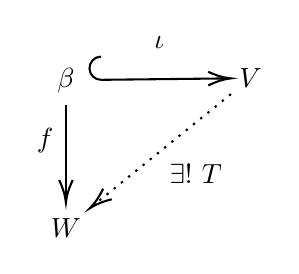
\begin{tikzpicture}[x=0.75pt,y=0.75pt,yscale=-1,xscale=1]
%uncomment if require: \path (0,235); %set diagram left start at 0, and has height of 235


% Text Node
\draw (228,104) node    {$\beta $};
% Text Node
\draw (317,103) node    {$V$};
% Text Node
\draw (228,175) node    {$W$};
% Text Node
\draw (218,133) node    {$f$};
% Text Node
\draw (288,149) node    {$^{\ } \exists !\ T$};
% Text Node
\draw (273,86) node    {$\iota $};
% Connection
\draw    (245,103.81) -- (305.5,103.13) ;
\draw [shift={(307.5,103.11)}, rotate = 179.36] [color={rgb, 255:red, 0; green, 0; blue, 0 }  ][line width=0.75]    (10.93,-3.29) .. controls (6.95,-1.4) and (3.31,-0.3) .. (0,0) .. controls (3.31,0.3) and (6.95,1.4) .. (10.93,3.29)   ;
\draw [shift={(245,103.81)}, rotate = 359.36] [color={rgb, 255:red, 0; green, 0; blue, 0 }  ][line width=0.75]      (0,-11.18) .. controls (-3.09,-11.18) and (-5.59,-8.68) .. (-5.59,-5.59) .. controls (-5.59,-2.5) and (-3.09,0) .. (0,0) ;
% Connection
\draw  [dash pattern={on 0.84pt off 2.51pt}]  (307.5,110.69) -- (241.05,164.44) ;
\draw [shift={(239.5,165.7)}, rotate = 321.03] [color={rgb, 255:red, 0; green, 0; blue, 0 }  ][line width=0.75]    (10.93,-3.29) .. controls (6.95,-1.4) and (3.31,-0.3) .. (0,0) .. controls (3.31,0.3) and (6.95,1.4) .. (10.93,3.29)   ;
% Connection
\draw    (228,116) -- (228,161) ;
\draw [shift={(228,163)}, rotate = 270] [color={rgb, 255:red, 0; green, 0; blue, 0 }  ][line width=0.75]    (10.93,-3.29) .. controls (6.95,-1.4) and (3.31,-0.3) .. (0,0) .. controls (3.31,0.3) and (6.95,1.4) .. (10.93,3.29)   ;

\end{tikzpicture}
\end{center}
\begin{itemize}
	\item $\beta$ es base de $V$
	\item Si $W$ es un $F-$espacio vectorial cualquiera, 
	toda función $f: \beta \longrightarrow W$ se puede extender
	linealmente de forma única a todo $V$, es decir, existe
	una única transformación lineal $T: V \longrightarrow W$
	tal que $T_{| \beta} = f$.
\end{itemize}
\end{teo}
\textbf{Nota:} en realidad, este teorema es cierto aún cuando
$V$ es infinito dimensional (c.f. \cite{Hugo} p. 84). Sin embargo,
como en el curso no hemos demostrado los resultados necesarios
para probar esto cuando se trabaja en un espacio infinito dimensional
(no estudiamos el Lema de Zorn, por lo que no pudimos demostrar
hechos fundamentales como la existencia de bases para cualquier
espacio vectorial o el hecho de que un l.i. de un espacio ininito
dimensional puede extenderse a una base de este), nos limitaremos
a establecer y probar la propiedad universal de las bases
en dimensión finita - que en realidad son los tipos de espacios
que se usan siempre en las aplicaciones.

\noindent
\textbf{Demostración.}
\begin{itemize}
	\item[$\Rightarrow )$] 
	Sea $f: \beta \longrightarrow W$ una función de la base
	$\beta = \{ v_{1}, \ldots , v_{n} \}$ 
	de $V$ escogida a $W$. Sean $x, y \in V$ cualesquiera;
	digamos que
	\begin{equation}
		\label{eq0: 25 sept}
		x = \sum_{i = 1}^{n} a_{i}v_{i}, \hspace{0.2cm}
		y = \sum_{i = 1}^{n} b_{i}v.
	\end{equation}
	Observe que, si $T: V \longrightarrow W$
	es una transformación lineal que extiende a $f$ (i.e.
	tal que $T \circ \iota = f$), entonces, deberá ocurrir
	\[
	T(x) = T \left( \sum_{i=1}^{n}a_{i}v_{i} \right)
	= \sum_{i=1}^{n} a_{i} T(v_{i})
	= \sum_{i=1}^{n} a_{i} \beta(v_{i}),
	\]
	es decir, $T$ \textit{tiene que ser} la función definida como
	\marginnote{Observe que la ecuación 
	\eqref{eq: definicion extension lineal de definicion en base} en efecto
	define una función $T$ de $V$ en $W$, pues, por ser $\beta$
	base de $V$, 
	la representación de $x$
	dada en \eqref{eq0: 25 sept} como combinaciones lineales de
	elementos de $\beta$ son únicas}
	\begin{equation}
		\label{eq: definicion extension lineal de definicion en base}
		T \left( \sum_{i=1}^{n}a_{i}v_{i} \right) := 
	\sum_{i=1}^{n} a_{i} \beta(v_{i}).
	\end{equation}
	Esta es en efecto una transformación lineal, pues
	\begin{align*}
	T(ax + y) = & T \left(a \sum_{i=1}^{n}a_{i}v_{i} +
	\sum_{i=1}^{n}b_{i}v_{i}\right) = T  
	\left(\sum_{i=1}^{n}(aa_{i} + b_{i} )v_{i} \right) \\
	= & \sum_{i=1}^{n} (aa_{i} + b_{i}) \beta(v_{i})
	= a\sum_{i=1}^{n} a_{i}\beta(v_{i}) + 
	\sum_{i=1}^{n} b_{i}\beta(v_{i}) = a T(x) + T(y),
	\end{align*}
	y, en efecto, $T \circ \iota = f$, pues, dado 
	$v_{i} \in \beta$ cualquiera,
	\[
	(T \circ \iota)(v_{i}) = T(v_{i}) =
	T (0v_{1} + \cdots + 1 v_{i} + \cdots + 0v_{n}) = f(v_{i}).
	\]
	\item[$\Leftarrow )$] 
	Mostremos que un subconjunto 
	$\beta = \{ v_{1}, \ldots , v_{n} \}$ de $V$ con tal propiedad
	es base de $V$.
	\begin{itemize}
		\item Independencia lineal: Supongamos que $v_{1} \in 
		\langle \beta - \{ v_{1} \} \rangle$, o sea, que existen
		escalares $c_{i}$ tales que 
		$v_{1} = \sum_{i=2}^{n}c_{i}v_{i}$. Sea la función
		$f: \beta \longrightarrow F$ definida como
		\[
		f(v_{1}) = 1, 
		\hspace{0.4cm} f(v_{i}) = 0,
		\hspace{0.2cm} 2 \leq i \leq n. 
		\]
		Sea $T$ la única extensión lineal de esta función.
		Se tiene que
		\[
		1 = T(v_{1}) = T \left( \sum_{i=2}^{n}c_{i}v_{i} \right)
		= \sum_{i=2}^{n} c_{i} T(v_{i}) = 
		\sum_{i=2}^{n} c_{i} 0_{W} = 0
		\hspace{0.2cm} \lightning 
		\]
		\item Generación: 
		Supongamos que $\beta$ no genera a $V$. Como 
		ya mostramos que $\beta$ es l.i., podemos extender $\beta$
		a una base de $V$ (c.f. corolario
		\ref{cor: extendiendo l.i. a base finita}).
		Sea pues $\gamma \subseteq V$ tal que 
		$\beta \cup \gamma$ es base de $V$. Si $f: \beta \longrightarrow V$
		se define como $f(v_{i}) = v_{i}$, observe que
		la función identidad $I_{V}: V \longrightarrow V$
		es tal que $I_{V} \circ \iota = f$, pero también la 
		proyección $T: V
		= \langle \beta \rangle
		\oplus \langle \gamma \rangle \longrightarrow V$ 
		definida como
		\[
		T(x) = b, \hspace{0.2cm} x = b + c, b \in \beta,
		c \in \gamma
		\]
		satisface que $T \circ \iota = f$. Como
		$T \neq I_{V}$, esto contradice la unicidad
		de la extensión lineal que suponemos por hipótesis.
	\end{itemize}
\end{itemize}

\QEDB
\vspace{0.2cm}

\marginnote{Es decir, para demostrar la igualdad entre transformaciones
lineales basta comprobar que sus definiciones en una base cualquiera
del dominio coinciden.}
\begin{cor}
	\label{cor: del teor fund bases}
Sea $V$, $W$ $F-$espacios vectoriales, con $V$ finito dimensional,
$T: V \longrightarrow W$, $U: V \longrightarrow W$ dos
transformaciones lineales. Si para una base
$\beta = \{ v_{1}, \ldots, v_{n} \}$ de $V$ se tiene que
\[
T(v_{i}) = U(v_{i}), \hspace{0.2cm} 1 \leq i \leq n,
\]
entonces $T = U$.
\end{cor}

Terminemos mostrando que todo $F-$espacio vectorial de 
dimensión $n$ es esencialmente $\IR^{n}$.

\begin{prop}
	\label{prop: dim V n sii V isomorfo a Rn}
Sea $V$ un $F-$ espacio vectorial. $V$ es $n-$dimensional
si y sólo si $V$ es isomorfo a $\IR^{n}$.
\end{prop}
\noindent
\textbf{Demostración.}
\begin{itemize}
	\item[$\Leftarrow$)] Inmediata de notar que $dim(\IR^{n}) = n$
	y la Proposición \ref{prop: isomorfo implica misma dimension}.
	\item[$\Rightarrow$)] Sea $\beta = \{ v_{1}, \ldots , v_{n} \}$
	base de $V$. Sea $f: \beta \longrightarrow \IR^{n}$ la función
	que a $v_{i}$ le asigna $\hat{e}_{i}$. Según la propiedad 
	universal de las bases (c.f. Teorema 
	\ref{teo: propiedad univ de las bases}), podemos extender
	a $\beta$ linealmente. Sea $T: V \longrightarrow \IR^{n}$ 
	tal extensión lineal. Puesto que $T(V)$ contiene a la 
	base canónica de $\IR^{n}$, $T(V) = \IR^{n}$, o sea,
	$T$ es suprayectiva. De esto, según el Teorema 
	\ref{teo: inyectiva sii supra sii biyect en dim finita}, se
	deduce que $T$ es un isomorfismo.
\end{itemize}
\QEDB
\vspace{0.2cm}

\section{Caracterización de transformaciones lineales de $\IR^{n}$ en $\IR^{m}$}
Es gracias a la propiedad universal de las bases establecida
en el Teorema \ref{teo: propiedad univ de las bases}
que vamos a poder caracterizar a las transformaciones lineales
entre $F-$espacios vectoriales finito
dimensionales. Como veremos más adelante, esto nos permitirá 
capturar toda la información de una transformación lineal a partir
de una cantidad finita de números, que almacenaremos en un arreglo
numérico rectangular - i.e. en una matriz.
Antes de abordar la teoría en general, para familiarizarnos
con las ideas que vamos a encontrar más adelante, estudiemos 
el caso de transformaciones lineales de un $\IR^{n}$
a un $\IR^{m}$, con $m, n \geq 1$ enteros.


Para simplificar la notación, conviene introducir la noción del
producto 
punto euclídeo en $\IR^{n}$.
\begin{defi}
Para $\hat{x} = (a_{i})_{i=1}^{n}, 
\hat{y} = (b_{i})_{i=1}^{n} \in \IR^{n}$, definimos su \textbf{producto
punto (euclídeo)} como
\[
\langle \hat{x}, \hat{y} \rangle = 
\sum_{i=1}^{n} a_{i} b_{i}.
\]
\end{defi}
Recordando la definición de producto de matrices, podemos
reinterpretar al producto punto de dos vectores de $\IR^{n}$
\marginnote{Este es un buen momento para recordar que, por lo general,
la multiplicación de matrices no es conmutativa.}
como producto de matrices;
\[
\langle \hat{x}, \hat{y} \rangle =
(a_{1}, a_{2}, \cdots , a_{n}) 
\begin{pmatrix}
b_{1} \\ b_{2} \\ \vdots \\ b_{n}
\end{pmatrix} 
= \left( \sum_{i=1}^{n}a_{i}b{i} \right).
\]
En lo que sigue, vamos a identificar
a una matriz de $1 \times 1$ con su única entrada.
Tampoco haremos distinción de los
``vectores fila''
$(a_{1}, a_{2}, \ldots , a_{n})$ con 
``vectores columna'' 
\[
\begin{pmatrix}
a_{1} \\ a_{2} \\ \vdots \\ a_{n}
\end{pmatrix}.
\]
Para ser más formales, deberíamos de escribir al 
vector columna anterior como $(a_{1}, \ldots , a_{n})^{t}$.

\begin{itemize}
	\item[$I)$] Sea $T : \IR \longrightarrow \IR^{n}$ lineal.
	Consideremos a la base $\{ 1 \}$ de $\IR$. Según el Teorema 
	\ref{teo: propiedad univ de las bases},
	$T$ queda completamente determinada por su valor en $1$;
	digamos que $T(1) = (c_{1}, c_{2}, \ldots , c_{n})$.
	Entonces, para toda $a \in \IR$ se tiene que 
	\[
	T(a) = T(a \cdot 1) = a T(1) = a(c_{1}, c_{2}, \ldots, c_{n})
	= \begin{pmatrix}
	c_{1} \\ c_{2} \\ \vdots \\ c_{n} 
	\end{pmatrix}
	(a).
	\]
	
	\item[$II)$] Sea $T: \IR^{n} \longrightarrow \IR$ lineal. Ahora vamos
	a considerar a la base canónica 
	$\{ \hat{e}_{1}, \hat{e}_{2}, \ldots , \hat{e}_{n} \}$
	de $\IR^{n}$. Nuevamente, el Teorema \ref{teo: propiedad univ de las bases}
	nos asegura que,
	con conocer los valores
	\begin{equation*}
		\label{eq: 0, 9 oct}
		c_{i} = T(\hat{e}_{i}) \in \IR, \hspace{0.3cm} 1 \leq i \leq n,
	\end{equation*}
	conocemos los valores de la transformación lineal $T$ en todo 
	punto de $\IR^{n}$; en efecto,
	si $\hat{x} = (a_{1}, a_{2}, \ldots , a_{n}) \in \IR^{n}$, entonces
	\[
	T(\hat{x}) = T\left( \sum_{i=1}^{n} a_{i}e_{i} \right)
	= \sum_{i=1}^{n} a_{i} T(e_{i}) = 
	\sum_{i=1}^{n} a_{i}c_{i} = \langle \hat{x}, \hat{c} \rangle
	= (c_{1}, c_{2}, \ldots, c_{n}) \begin{pmatrix}
	a_{1} \\ a_{2} \\ \vdots \\ a_{n}
	\end{pmatrix},
	\]
	donde $\hat{c} = (c_{1}, c_{2}, \ldots ,c_{n})$.
	\item[$II)$] Ahora sí, consideremos el caso más general de 
	una transformación lineal $T: \IR^{n} \longrightarrow \IR^{m}$,
	con $m, n \geq 1$ enteros cualesquiera.
	De nuevo tomamos a la base canónica de $\IR^{n}$ compuesta
	por los vectores $\hat{e}_{i}$. Si 
	\[
	T(e_{i}) = (c_{1i}, c_{2i} \ldots , c_{mi}),
	\hspace{0.3cm} 1 \leq i \leq n,
	\]
	entonces,
	para cualquier $\hat{x} = (a_{1}, \ldots , a_{n}) \in \IR^{n}$,
	\begin{align*}
	T(\hat{x}) = 
	T\left( \sum_{i=1}^{n} a_{i}e_{i} \right) 
	= & \sum_{i=1}^{n} a_{i} T(e_{i})
	\\
	= &
	\sum_{i=1}^{n} a_{i}(c_{1i}, c_{2i}, \ldots, c_{mi}) \\ 
	= & \sum_{i=1}^{n}(a_{i}c_{1i}, a_{i} c_{2i}, \ldots , a_{i}c_{mi})\\
	= & \left( \sum_{i=1}^{n} a_{i}c_{1i},
	\sum_{i=1}^{n} a_{i}c_{2i}, \ldots , 
	\sum_{i=1}^{n} a_{i}c_{mi}  \right) \\
	= & \left(
	\langle \hat{x}, M_{1}\rangle, 	 
	\langle \hat{x}, M_{2}\rangle, \ldots ,
	\langle \hat{x}, M_{m}\rangle
	\right),
	\end{align*}
	donde $M_{1}, M_{2}, \ldots , M_{m}$ son las $m$
	filas de la matriz
	\[
	\begin{pmatrix}
	c_{11} & c_{12} & \ldots & c_{1n} \\
	c_{21} & c_{22} & \ldots & c_{2n} \\
	\cdots & \cdots & \cdot & \cdot \\
	c_{m1} & c_{m2} & \cdots & c_{mn}
	\end{pmatrix} \in M_{m \times n}(\IR),
	\]
que se forma usando a los $n$ vectores $T(e_{i})$ de $\IR^{m}$ 
como columnas.
\end{itemize}
\newpage
\section{Ejercicios III}

Demos un repaso de los conceptos estudiados.

\textbf{I )} Construyamos una base de $\IR^{3}$ que contenga al vector $v_{1} = (4, 5, 9)$.
\begin{itemize}
	\item Para que $v_{2}$ sea tal que $\{ v_{1}, v_{2} \}$ sea l.i.,
	debe cumplirse que 
	\marginnote{Para esta construcción estamos usando el Lema
	\ref{lema: S union x es ld sii x en generado de S}.}
	\[
	v_{2} \in \IR^{3} - span(\{ v_{1} \}), 
	\]
	es decir, que $v_{2}$ no sea múltiplo escalar de $v_{1}$. Pongamos pues
	a $v_{2} = (5, 3, 7)$.
	\item Para que $v_{3}$ sea tal que $\{ v_{1}, v_{2}, v_{3} \}$ 
	sea l.i., se deberá tener 
	\begin{align*}
	v_{3} \in \IR^{3} - span(\{ v_{1}, v_{2} \} )
	= &
	\IR^{3} - \{ a(4, 5, 9) + b (5, 3, 7) : \hspace{0.2cm} a, b \in \IR \} \\
	= & 
	\IR^{3} - \{ (4a+5b, 5a+3b, 9a+7b)  | \hspace{0.2cm} a, b \in \IR \}.
	\end{align*}
	Haciendo $a = 1$, $b = -1$, tenemos que el vector 
	$(-1, 2, 2)$ es elemento de $span(\{ v_{1}, v_{2} \})$; cambiando
	una de las tres entradas obtendremos un vector que no está en este
	espacio (pues el sistema planteado para expresar a este nuevo vector
	como combinación lineal de $v_{1}$ y $v_{2}$ no tendría solución,
	recuerde el Teorema de Cramer). Tomemos pues a $v_{3} = (-1, 2, 0)$.
\end{itemize}
Obtuvimos así al subconjunto linealmente independiente
\[
\beta = 
\{ v_{1} = (4, 5, 9), v_{2} = (5, 3, 7), v_{3} = (-1, 2, 0) \}
\]
de $\IR^{3}$; como este tiene tres elementos y la dimensión de 
$\IR^{3}$ es $3$, tenemos que es una base de $\IR^{3}$.

\textbf{II)}Encontremos ahora, usando el argumento de la demostración
del Teorema fundamental de las bases
\ref{teo: propiedad univ de las bases}, una transformación
lineal $T: \IR^{3} \longrightarrow \IR^{2}$ tal que 
\begin{equation}
	\label{eq: condiciones para T ejemplo}
	T(v_{1}) = (1, 0), \hspace{0.2cm}
	T(v_{2}) = (2, 5), \hspace{0.2cm}
	T(v_{3}) = (-3, 1).
\end{equation}
Tenemos primero que ver cómo expresar a cualquier vector
$(x, y, z) \in \IR^{3}$ como combinación lineal de elementos
de la base $\beta$. Estamos buscando entonces a los únicos
escalares $a, b, c \in \IR$ tales que 
\begin{align*}
(x, y, z) = & a (4, 5, 9) + b (5, 3, 7) + c(-1, 2, 0) \\
= & (4a+5b-c, 5a+3b+2c, 9a+7b).
\end{align*}
Esta igualdad en $\IR^{3}$ es equivalente al sistema de ecuaciones
que resolvemos a continuación:
\marginnote{En este argumento, $x$, $y$ y $z$ son las constantes,
mientras que las incógnitas son los escalares $a$, $b$ y $c$.}
\begin{align*}
\left( \begin{array}{rrr|r} 
4 & 5 & -1 & x  \\ 
5 & 3 & 2 & y  \\ 
9 & 7 & 0 & z
\end{array} \right) \sim &
\left( \begin{array}{rrr|r} 
1 & 5/4 & -1/4 & x/4  \\ 
5 & 3 & 2 & y  \\ 
9 & 7 & 0 & z
\end{array} \right) \sim &
\left( \begin{array}{rrr|r} 
1 & 5/4 & -1/4 & x/4  \\ 
0 & -13/4 & 13/4 & y - 5x/4  \\ 
0 & -17/4 & 9/4 & z-9x/4
\end{array} \right) 
\end{align*}
\begin{align*}
\sim
\left( \begin{array}{rrr|r} 
1 & 5/4 & -1/4 & x/4  \\ 
0 & 1 & -1 & -4y/13 + 5x/13  \\ 
0 & -17 & 9 & 4z-9x
\end{array} \right) \sim &
\left( \begin{array}{rrr|r} 
1 & 5/4 & -1/4 & x/4  \\ 
0 & 1 & -1 & -4y/13 + 5x/13  \\ 
0 & 0 & 8 & -4z+68y/13 - 32x/13
\end{array} \right) .
\end{align*}
Tenemos entonces que
\marginnote{\hlgray{Ejercicio:} sustituyendo algunos valores
para $x$, $y$ y $z$ compruebe que las fórmulas
\eqref{eq: ejemplo c}, \eqref{eq: ejemplo b} y
\eqref{eq: ejemplo a} son correctas.}
\begin{equation}
	\label{eq: ejemplo c}
	c = -\frac{1}{8} \left( 4z - \frac{68}{13} y
- \frac{32}{13} x \right) = 
\frac{4}{13} x + \frac{17}{26} y - \frac{1}{2} z,
\end{equation}
\begin{equation}
	\label{eq: ejemplo b}
	b = c - \frac{4}{13} y + \frac{5}{13} x =
\frac{9}{13} x + \frac{9}{26} y - \frac{1}{2} z,
\end{equation}
y
\begin{equation}
	\label{eq: ejemplo a}
	a = \frac{1}{4} \left( x+c-5b \right)
= -\frac{7}{13} x - \frac{7}{26} y + \frac{1}{2} z.
\end{equation}
Usando estas tres expresiones, tenemos que
la única transformación que extiende la definición 
\eqref{eq: condiciones para T ejemplo}
en la base $\beta$ es
\marginnote{\hlgray{Ejercicio:} compruebe que la transformación
lineal propuesta cumple las condiciones 
\eqref{eq: condiciones para T ejemplo}.}
\begin{align*}
T(x, y, z) = & 
T \left( a v_{1} + bv_{2} + cv_{3} \right) \\
= & a T(v_{1}) + b T(v_{2}) + c T(v_{3}) \\
= & \left( -\frac{7}{13} x - \frac{7}{26} y + \frac{1}{2} z \right)
(1, 0) + 
\left( \frac{9}{13} x + \frac{9}{26} y - \frac{1}{2} z \right)
(2, 5) + 
\left( \frac{4}{13} x + \frac{17}{26} y - \frac{1}{2} z \right)
(-3, 1) \\
= & \left( -\frac{1}{13} x - \frac{20}{13} y + z,
\frac{49}{13}x + \frac{31}{13} y - 3z \right).
\end{align*}


\begin{ej}
	\label{ej: operaciones entre lineales}
Sean $U$, $V$ y $W$ tres $F-$espacios vectoriales, $a \in F$.
Demuestra que
\begin{itemize}
	\item Si $f, g: V \longrightarrow W$ son transformaciones lineales, 
	entonces $f+g$ y $af$ son transformaciones lineales.
	\item Si $f: V \longrightarrow W$ y $g: W \longrightarrow U$
	son transformaciones lineales, la función composición
	$g \circ f : V \longrightarrow U$ es también lineal.
\end{itemize}
\end{ej}

\begin{ej}
Argumente por qué
existe una única transformación lineal $T: \IR^{2} \longrightarrow \IR^{3}$
tal que 
\[
T(2, 5) = (1, 0, 1), \hspace{0.2cm}
T(-1, 4) = (2, 5, 7)
\]
y de su fórmula explícitamente.
\end{ej}

\begin{ej}
Argumente por qué
existe una única transformación lineal $T: P_{2}(\IR) \longrightarrow 
P_{2}(\IR)$
tal que 
\[
T(1) = x^{2}, \hspace{0.2cm}
T(1+x) = 2x, \hspace{0.2cm}
T(x^{2}-1) = 2.
\]
y de su fórmula explícitamente.
\end{ej}

\newpage
\chapter{Representaciones matriciales de transformaciones lineales}


\begin{signquote}{Mac Lane, 1954}
	The proper treatment of calculus for functions of 
	several variables requires vector ideas; the budding statistician and
	the coming physicist need them; modern 
	analysis is unthinkable without the notion of linear
	dependence and all that flows from it. Throughout these
	courses the infusion of a geometrical point of view is of paramount 
	importance. A vector is geometrical; it is an element of a vector space,
	defined by suitable axioms - whether the scalars be real numbers or
	elements of a general field. A vector is not an n-tuple of numbers
	until a coordinate system has been chosen. Any teacher and any
	text book which starts with the idea that vectors are
	n-tuples is committing a crime for which the proper punishment is ridicule.
	The n-tuple idea is not ``easier'', it is harder; it is not clearer, it is
	more misleading. 
\end{signquote}
\marginnote{Podrá notar que, en lo que sigue, siempre que se defina
	un concepto para transformaciones lineales, se intentará traducir y relacionar
	con uno para matrices. Estaremos constantemente estudiando la relación entre
	espacios de transformaciones lineales con espacios matriciales.}
	
\vspace{1cm}

\begin{signquote}{Keith van Rijsbergen}
	Now imagine that the query is
	simply an abstract vector in the space, we would still have to define it
	with respect to the basis of the space, but it would be up to us, or the
	user, to refer the objects in the space to different bases depending on
	their point of view. A change of basis constitutes a change of point of
	view.
\end{signquote}



\label{chapter: representaciones matriciales de transformaciones lineales}
Desarrollada la teoría de transformaciones lineales en
el capítulo anterior, nos proponemos ahora usar la propiedad
universal de las bases (c.f. Teorema
\ref{teo: propiedad univ de las bases}) para representar 
transformaciones lineales entre espacios vectoriales finito dimensionales
con matrices. 

\begin{itemize}
	\item Mostraremos que, 
	fijando bases en los espacios de salida y de llegada,
	podremos establecer una biyección (que de hecho será un isomorfismo)
	que identificará una transformación lineal entre estos espacios
	con una matriz. 
	\item Puesto que esta asociación preserva estructura, podremos 
	realizar operaciones con matrices (que son objetos sencillos de 
	almacenar y operar en una computadora) e interpretarlas como
	operaciones entre transformaciones lineales.
\end{itemize}

Antes de explicar cómo almacenar la información de una transformación
lineal en una matriz - situación que implicará trabajar con
un $F-$ espacio vectorial de matrices con coeficientes
en $F$ - estudiemos la estructura del espacio de transformaciones lineales. 

\section{El espacio $\mathcal{L}(V, W)$}
A partir de ahora vamos a considerar dos $F-$espacios vectoriales
$V$ y $W$, con 
\[
dim(V) = n, \hspace{0.3cm} dim(W) = m,
\]
y
\[
\beta= \{ v_{1}, \ldots , v_{n} \} \subseteq V, 
\hspace{0.3cm}
\gamma = \{ w_{1}, \ldots , v_{m} \} \subseteq W
\]
bases de estos. 

\begin{prop}
Definiendo la suma y multiplicación escalar puntualmente, 
\[
\mathcal{L} (V, W) :=
\{ T: V \longrightarrow W  | \hspace{0.2cm} \textit{ T es lineal}  \}
\]
es un $F-$espacio vectorial. 
\end{prop}
\noindent
\textbf{Demostración.}
\hlgray{Ejercicio.} Como sugerencia, considere a 
\[
X = 
\{ T: V \longrightarrow W  | \hspace{0.2cm} \textit{ T es función} \}.
\]
Por herencia de $W$, $X$ es un $F-$espacio vectorial.
Si demuestra que el subconjunto $\mathcal{L}(V, W)$ de $X$
es no vacío, cerrado bajo sumas y multiplicación escalar
(c.f. ejercicio \ref{ej: operaciones entre lineales}), entonces
tendrá que es subespacio de $X$ - luego, espacio vectorial en
sí mismo.
\QEDB
\vspace{0.2cm}

En $W$ no se tiene definida una multiplicación, por lo que no tendría
sentido definir el produco de transformaciones lineales
puntualmente, sin embargo, siempre podemos componer funciones:
recuerda que, 
si $T : V_{1} \longrightarrow V_{2}$, $U: V_{2} \longrightarrow V_{3}$
son transformaciones lineales, 
su composición $ U \circ T : V_{1} \longrightarrow V_{3}$ se define como
\[
(U \circ T)(v) = U(T(v)), \hspace{0.3cm} v \in V_{1}.
\]
\begin{prop}
	La composición de transformaciones lineales es una transformación lineal.
\end{prop}
\textbf{Demostración.}
\hlgray{Ejercicio.}
\QEDB
\vspace{0.2cm}



\section{El isomorfismo $[\cdot]_{\beta}$}
A partir de ahora, fijada una base $\beta$ de un 
$F-$espacio vectorial $V$, nos interesarán no sólo sus elementos, sino
también el orden en el que estos se enlistan.
Por eso, ahora que digamos ``base'', nos estaremos refiriendo
a una ``base ordenada''. Por ejemplo,
\[
\beta_{1} = \{ (1, 0), (0, 1) \} \hspace{0.2cm}
\textit{ y }
\hspace{0.2cm}
\beta_{1} = \{ (0, 1), (1, 0) \}
\]
son, como conjuntos, iguales, pero como bases
ordenadas de $\IR^{2}$ son distintas.

\begin{defi}
Sea $V$ un $F-$espacio vectorial
$n-$dimensional, $\beta = \{ v_{1}, \ldots, 
v_{n} \}$ una base de este. Para $x \in V$, si 
$x = \sum_{i=1}^{n}a_{i}v_{i}$ es la única representación de 
$x$ como combinación lineal de elementos de $\beta$, entonces,
al vector de $\IR^{n}$
\begin{equation}
	\label{eq: vector coordenado de x}
	[x]_{\beta} = \begin{pmatrix}
a_{1} \\ a_{2} \\ \vdots \\ a_{n}
\end{pmatrix} \in \IR^{n}
\end{equation}
se le llamará el \textbf{vector coordenado de $x$ respecto a $\beta$}.
\end{defi}

Observe que la asignación
\[
x \mapsto [x]_{\beta}
\]
de $V$ en $F^{n}$ es una función, pues la representación de
cada vector en $V$ como combinación lineal de elementos de 
$\beta$ es única (luego, a cada vector le estamos asignando una
y sólo una columna ordenada).
De hecho, $[\cdot]_{\beta}$
es la transformación lineal usada en 
la demostración de la Proposición
\ref{prop: dim V n sii V isomorfo a Rn} para demostrar que,
si $V$ tiene dimensión $n$, entonces es isomorfo a 
$\IF^{n}$. \textbf{Usando entonces a la base $\beta$ de $V$, estamos
identificando a cada vector de $V$ con una $n-$tupla via
este isomorfismo}. 
Esto es útil pues, aunque los elementos del
espacio original $V$ no sean elementos de $\IR^{n}$, si $V$ es
de dimensión finita, ¡los podemos
identificar como tal!

\begin{prop}
	Sean $V$ un $F-$espacio vectorial de dimensión $n$, 
$\beta = \{ v_{1}, v_{2}, \ldots, v_{n} \}$ una base de $V$, y 
$[\cdot]_{\beta}: V \longrightarrow \IR^{n}$ la transformación lineal
dada por 
\eqref{eq: vector coordenado de x}.
\begin{itemize}
	\item $[\cdot]_{\beta}$ es un isomorfismo. En particular,
	\[
	[x]_{\beta} = [y]_{\beta} \Rightarrow x = y.
	\]
	\item Para toda $1 \leq i \leq n$, $[v_{i}]_{\beta} = e_{i}$, 
	el i-ésimo vector de la base canónica de $\IR^{n}$.
\end{itemize}
\end{prop}

Note que la identificación \eqref{eq: vector coordenado de x}
de un vector del espacio con un elemento de $\IR^{n}$ depende de 
la base $\beta$ fijada. 

\hlgray{Ejercicio:} 
Sean $V$ un $F-$espacio vectorial finito dimensional, 
$\beta, \gamma$ bases de este distintas entre sí.
Demuestre que, 
\begin{itemize}
	\item existe $x \in V$ tal que 
	$[x]_{\beta} \neq [x]_{\gamma}$, y que 
	\item $[x]_{\beta} = [y]_{\gamma}$ no necesariamente implica 
	$x = y$.
\end{itemize}


\begin{nota}
	Fijada una base $\beta = \{ v_{1}, \ldots , v_{n} \}$ de $V$, 
	es importante recordar la definición del isomorfismo $[\cdot]_{\beta}$;
	\marginnote{En \eqref{eq: def del iso asociado a beta}, 
	nota que la ecuación de la derecha es en $V$, y la ecuación de la izquierda
	es en $F^{n}$.}
	\begin{equation}
			\label{eq: def del iso asociado a beta}
			\forall x \in V: 
			\hspace{0.2cm}
			[x]_{\beta} = (a_{1}, \ldots , a_{n}) \hspace{0.2cm}
			\textit{si y sólo si } \hspace{0.2cm}
			x = a_{1} v_{1} + \cdots + a_{n} v_{n},
	\end{equation}
	pues es con ella que recuperamos al vector $x \in V$
	a partir de la $n-$tupla $(a_{1}, \ldots , a_{n}) \in F^{n}$.
\end{nota}

\hlgray{Ejercicio:} resuelve los ejercicios 1 a 5
de la lista \ref{sec: ejercicios iv}.



\section{Representación matricial de una transformación lineal}

Vamos a considerar ahora a dos $F-$espacios vectoriales finito 
dimensionales
\[
V, \hspace{0.2cm} dim(V) = n,\beta = \{ v_{1}, \ldots, v_{n} \}
\subseteq V \hspace{0.1cm} \textit{ base de }V,
\]
\[
W, \hspace{0.2cm} dim(V) = n,\gamma = \{ w_{1}, \ldots, w_{m} \}
\subseteq W \hspace{0.1cm} \textit{ base de }W.
\]

Recuerde que, si $T: V \longrightarrow W$ es una transformación lineal,
entonces
\begin{itemize}
	\item Por el Teorema fundamental de las bases 
	\ref{teo: propiedad univ de las bases}, 
	la transformación $T$ queda completamente
	\marginnote{En esta discusión, ``$i$'' es la variable con la que
	contamos a los elementos de la base $\beta$, y com ``$j$'' contamos
	a los elementos de la base $\gamma$.}
	determinada por los valores que toma en la base $\beta$ de $V$,
	es decir, a partir de los valores
	\[
	T(v_{i}), \hspace{0.2cm} 1 \leq i \leq n
	\]
	podemos recuperar la definición de $T$ \textit{en todo el espacio
	$V$}.
	\item Por ser $\gamma$ base de $W$, cada $T(v_{i})$ puede
	expresarse de forma única como combinación lineal de 
	los vectores $w_{1}, \ldots, w_{m}$, es decir,
	para cada $1 \leq i \leq n$, existen únicos escalares
	$a_{ji}$ tales que
	\marginnote{Nota que en la ecuación \eqref{eq: 24 oct, 1} se fija
	el segundo índice de los escalares, es decir, el índice columna.}
	\begin{equation}
		\label{eq: 24 oct, 1}
	T(v_{i}) = \sum_{j = 1}^{m} a_{ji} w_{j}, 
	\hspace{0.2cm} 1 \leq i \leq n.
	\end{equation}
\end{itemize}
Así, una vez fijadas las bases $\beta$ y $\gamma$, 
\textbf{la transformación lineal $T$ queda completamente determinada
por los $m \times n$ escalares $a_{ji}$, con $1 \leq i \leq n$ y
$1 \leq j \leq m$}. Almacenamos esta información en la siguiente
matriz:

\begin{equation}
	\label{eq: representacion matricial T}
	[T]_{\beta}^{\gamma} = 
	\begin{pmatrix}
	a_{11} & a_{12} & \ldots & a_{1n} \\
	a_{21} & a_{22} & \ldots & a_{2n} \\
	\vdots & \vdots & \ddots & \vdots \\
	a_{m1} & a_{m2} & \ldots & a_{mn} 
	\end{pmatrix}.
\end{equation}
\begin{marginfigure}
	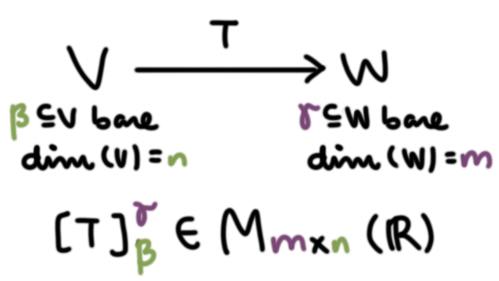
\includegraphics[scale= 1.9]{19} 
\end{marginfigure}
Note que la $i-$ésima columna de $[T]_{\beta}^{\gamma}$
es el vector columna $[T(v_{i})]_{\gamma}$. Entonces,
\begin{itemize}
	\item La matriz $[T]_{\beta}^{\gamma}$ tiene $n$ columnas,
	pues hay una por cada elemento de la base $\beta$ de $V$, y
	\item tiene $m$ filas, pues cada vector columna tiene $m$ 
	entradas, a saber, los coeficientes de las combinaciones
	lineales de las imágenes $T(v_{i})$ respecto a $\gamma$.
\end{itemize}

\begin{figure}[H]
	\sidecaption{
	Este diagrama puede ayudarte a recordar cómo se construye
	la matriz
	$[T]_{\beta}^{\gamma}$
	\label{fig: diagrama representacion matr}
	}
	\centering
	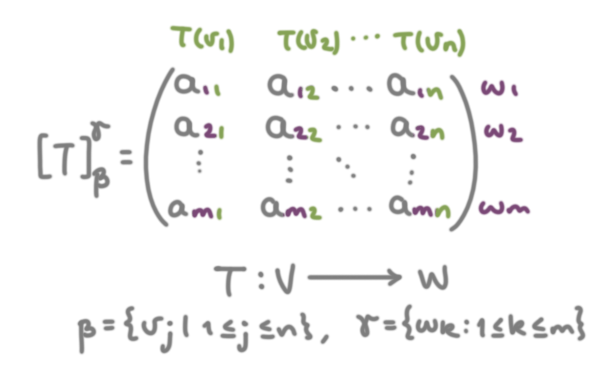
\includegraphics[scale = 2.7]{20} 
\end{figure}	



\section{El isomorfismo $\Phi_{\beta}^{\gamma}$}
\label{sect: iso phi}
\hlpink{Agregar nota de iso de anillos: Golan.}


Fijadas bases $\beta = \{ v_{j}  | \hspace{0.2cm} 1 \leq j \leq n \}
\subseteq V$ y $\gamma 
= \{ w_{k}  | \hspace{0.2cm} 1 \leq k \leq m \} 
\subseteq W$ de dos 
$F-$espacios finito dimensionales, vamos a establecer una biyección
entre
\begin{itemize}
	\item el espacio $\mathcal{L}(V, W)$ de transformaciones lineales
	de $V$ en $W$ y 
	\item el espacio de matrices $M_{m \times n}(F)$.
\end{itemize}
Denotemos por 
$\Phi_{\beta}^{\gamma}$ a la función que a cada 
transformación lineal de $V$ en $W$ le asigna su representación
matricial respecto a $\beta$ y $\gamma$, es decir, 
\[
\Phi_{\beta}^{\gamma} : \mathcal{L}(V, W) \longrightarrow M_{m \times n}(F)
\]
\[
\Phi_{\beta}^{\gamma}(T) = [T]_{\beta}^{\gamma}.
\]

Del Teorema fundamental de las bases se sigue de inmediato
que $\Phi_{\beta}^{\gamma}$ 
la función 
es una biyección. 

\begin{prop}
	La función $\Phi_{\beta}^{\gamma}$ es una biyección.
\end{prop}
\noindent
\textbf{Demostración.}
\begin{itemize}
	\item \textbf{Inyectividad de $\Phi_{\beta}^{\gamma}$}:
	Sean $T, U : V \longrightarrow W$ lineales tales que 
	\marginnote{En la demostración de la inyectividad de $\Phi_{\beta}^{\gamma}$,
		queremos inferir una igualdad de funciones a partir de una igualdad de matrices.}
	\[
	[T]_{\beta}^{\gamma} = \Phi_{\beta}^{\gamma}(T)
	= \Phi_{\beta}^{\gamma}(T) = [U]_{\beta}^{\gamma}.
	\]
	El que las matrices $[T]_{\beta}^{\gamma}$ y 
	$[U]_{\beta}^{\gamma}$ sean iguales significa que 
	\[
	\forall v \in \beta : \hspace{0.2cm} T(v) = U(v),
	\]
	pues la $j-$ésima columna de la matriz
	$[T]_{\beta}^{\gamma}$ (respectivamente, de 
	$[U]_{\beta}^{\gamma}$), 
	da los coeficientes 
	de la combinación lineal en términos de $\gamma$ igual a $T$ 
	(respectivamente, $U$)
	evaluada en el
	$j-$ésimo vector de la base $\beta$. Así, $T$ y $U$ coinciden en la 
	base $\beta$ de $V$, luego, según el Corolario 
	\ref{cor: del teor fund bases}, coinciden.
	\item \textbf{Suprayectividad de $\Phi_{\beta}^{\gamma}$}:
	sea $A = (a_{ij}) \in M_{m \times n}(F)$. Por el Teorema fundamental 
	de las bases, 
	existe una única
	transformación lineal tal que 
	\[
	T(v_{j}) = \sum_{k = 1}^{m} a_{kj} w_{j}, \hspace{0.3cm}
	1 \leq j \leq n.
	\]
	Dicha $T$ es tal que $[T]_{\beta}^{\gamma} = A$.
\end{itemize}

\QEDB
\vspace{0.2cm}




\textbf{Nota:} se pidió a partir de ahora que las bases de los
espacios vectoriales considerados fuesen ordenadas pues,
para la construcción de las representaciones matriciales 
$[T]_{\beta}^{\gamma}$, la $j-$ésima columna corresponde al
$j-$ésimo vector de la base $\beta$, luego, el orden en el que se
enlistan los elementos de $\beta$ importa (es cierto que un cambio
de orden en los elementos de un conjunto no afecta su identidad,
pero, el cambiar el orden de las entradas de una matriz 
definitivamente la 
altera).
El orden de las columnas de una representación matricial 
$A$ está directamente relacionado con el orden de los vectores en 
una base ordenada.


\begin{figure}[H]
	\centering
	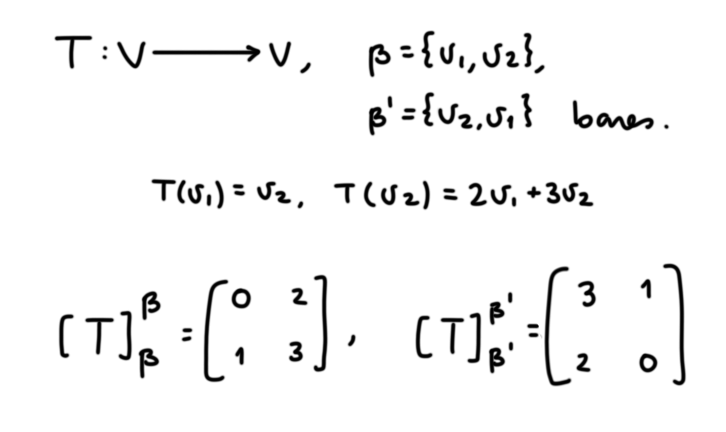
\includegraphics[scale = 2.3]{ 31} 
\end{figure}	


En la siguiente sección desarrollaremos la teoría suficiente
para demostrar que, más que una biyección, $\Phi_{\beta}^{\gamma}$
es un isomorfismo. Esto implica que el espacio
$\mathcal{L}(V, W)$ de transformaciones lineales entre
dos espacios finito dimensionales es, 
salvo isomorfismo, un espacio de matrices. En lo que sigue,
seguiremos estudiando y explotando la relación entre 
estos 
dos espacios,
para interpretar las operaciones que realicemos en uno en
términos de operaciones en el otro espacio (pues, para las aplicaciones,
es muchísimo más sencillo trabajar con matrices a lidiar
con transformaciones lineales entre espacios que, a pesar de ser
finito dimensionales, pueden ser complicados).



\section{Operaciones entre transformaciones lineales usando sus representaciones matriciales}


Empecemos estableciendo la linealidad de la biyección
$\Phi_{\beta}^{\gamma}$ estudiada en 
la Sección \ref{sect: iso phi}.


\begin{prop}
Sean
$V$ y $W$ dos $F-$espacios vectoriales con $\beta = \{ v_{1}, \ldots , 
v_{n} \} \subseteq V$ y 
$\gamma = \{ w_{1}, \ldots , w_{m}\} \subseteq W$ bases de estos. 
\marginnote{Nota que el lado izquierdo de 
\eqref{eq: suma de matrices transf lin} involucra una suma de funciones,
mientras que el lado derecho es una suma de matrices.}
Para cualesquiera $T, U :V \longrightarrow W$
y $\lambda \in F$, 
\begin{equation}
	\label{eq: suma de matrices transf lin}
	[T + U]_{\beta}^{\gamma} = [T]_{\beta}^{\gamma} + 
[U]_{\beta}^{\gamma}.
\end{equation}
\begin{equation}
	\label{eq: mult escalar de matrices transf lin}
	[\lambda T]_{\beta}^{\gamma} = \lambda [T]_{\beta}^{\gamma}.
\end{equation}
\end{prop}
\textbf{Demostración.}
Digamos que
\[
[U]_{\gamma}^{\delta} = 
\begin{pmatrix}
	a_{11} & a_{12} & \ldots & a_{1n} \\
	a_{21} & a_{22} & \ldots & a_{2n} \\
	\vdots & \vdots & \ddots & \vdots \\
	a_{m1} & a_{m2} & \ldots & a_{mn}
\end{pmatrix},
\hspace{0.2cm}
[T]_{\beta}^{\gamma} = 
\begin{pmatrix}
	b_{11} & b_{12} & \ldots & b_{1n} \\
	b_{21} & b_{22} & \ldots & b_{2n} \\
	\vdots & \vdots & \ddots & \vdots \\
	b_{m1} & b_{m2} & \ldots & b_{mn}
\end{pmatrix}.
\]
De estas representaciones matriciales inferimos que,
para toda $1 \leq j \leq n$,
\[
U(v_{j}) = \sum_{k=1}^{m} a_{kj} w_{k},
\hspace{0.2cm}
T(v_{j}) = \sum_{k=1}^{m} b_{kj} w_{k},
\]
luego,
\[
(T + U)(v_{j}) = \sum_{k=1}^{m} b_{kj} w_{k} +
\sum_{k=1}^{m} a_{kj} w_{k}
= \sum_{k=1}^{m} (b_{kj} + a_{kj}) w_{k},
\]
y
\[
(\lambda T)(v_{j}) = 
\lambda \left( \sum_{k=1}^{m} b_{kj} w_{k} \right) 
= \sum_{k=1}^{m} (\lambda b_{kj}) w_{k},
\]
por lo tanto,

\[
[T + U]_{\beta}^{\gamma} = 
\begin{pmatrix}
	b_{11} + a_{11} & b_{12} + a_{12} & \ldots & b_{1n} + a_{1n} \\
	b_{21} + a_{21} & b_{22} + a_{22} & \ldots & b_{2n} + a_{2n} \\
	\vdots & \vdots & \ddots & \vdots \\
	b_{m1} + a_{m1} & b_{m2} + a_{m2} & \ldots & b_{mn} + a_{mn}
\end{pmatrix}
= [T]_{\beta}^{\gamma} + [U]_{\beta}^{\gamma},
\]
y 
\[
[\lambda T]_{\beta}^{\gamma}
= 
\begin{pmatrix}
	\lambda b_{11} & \lambda b_{12} & \ldots & \lambda b_{1n} \\
	\lambda b_{21} & \lambda b_{22} & \ldots & \lambda b_{2n} \\
	\vdots & \vdots & \ddots & \vdots \\
	\lambda b_{m1} & \lambda b_{m2} & \ldots & \lambda b_{mn}
\end{pmatrix}
\]
\QEDB
\vspace{0.2cm}

\marginnote{
Si $V$ y $W$ son finito dimensionales, 
$\mathcal{L}(V, W)$ es un espacio de funciones 
finito dimensional.
}

\begin{cor}
	Sean $V$, $W$ dos $F-$espacios vectoriales, con 
	$dim(V) = n$, $dim(W) = m \in \IN$. Si 
	$\beta \subseteq V$, $\gamma \subseteq W$
	son bases de estos espacios, entonces, la función
	\[
	\Phi_{\beta}^{\gamma} : \mathcal{L}(V, W) \longrightarrow M_{m \times n}(F)
	\]
	\[
	\Phi_{\beta}^{\gamma}(T) = [T]_{\beta}^{\gamma}.
	\]
	es un isomorfismo.
\end{cor}

\begin{cor}
	Si $dim(V) = n, dim(W) = m \in \IN$, entonces
	$dim(\mathcal{L}(V, W)) = m n $.
\end{cor}


\begin{prop}
	\label{prop: calculo de composicion de transf a partir de producto de matr}
Sean $V$, $W$ y $Z$ tres $F-$espacios vectoriales,
con
$\beta = \{ v_{j} : \hspace{0.2cm} 1 \leq j \leq n \} \subseteq V$,
$\gamma = \{ w_{k}: \hspace{0.2cm} 1 \leq k \leq m \} \subseteq W$
y $\delta = \{ z_{i}: \hspace{0.2cm} 1 \leq i \leq r \}$
bases de estos. Si
\marginnote{Nota que el lado izquierdo de 
\eqref{eq: multipl de matrices transf lin} involucra una 
composición de funciones,
mientras que el lado derecho es un producto de matrices.
De hecho, el producto de matrices se definió de tal forma que
la ecuación \eqref{eq: multipl de matrices transf lin} fuese cierta.}
$T: V \longrightarrow W$ y $U: W \longrightarrow Z$ son lineales,
entonces
 \begin{equation}
	\label{eq: multipl de matrices transf lin}
	[U \circ T]_{\beta}^{\delta} = [U]_{\gamma}^{\delta} \cdot  
[T]_{\beta}^{\gamma}.
\end{equation}
\end{prop}
\noindent
\textbf{Demostración.}
Tenemos que $[U]_{\gamma}^{\delta} \in M_{r \times m}(\IR)$
y que $[T]_{\beta}^{\gamma} \in M_{m \times n}(\IR)$, por lo tanto, 
el producto de matrices en 
\eqref{eq: multipl de matrices transf lin} está bien definido.
\begin{center}
$[U]_{\gamma}^{\delta}$ tiene $1 \leq i \leq r$ filas y 
$1 \leq k \leq m$ columnas,
\end{center}
\begin{center}
$[T]_{\beta}^{\gamma}$ tiene $1 \leq k \leq m$ filas y 
$1 \leq j \leq n$ columnas;
\end{center}
entonces,
\begin{center}
$[U \circ T]_{\beta}^{\delta}$ tiene $1 \leq i \leq r$ filas y 
$1 \leq j \leq n$ columnas.
\end{center}

\begin{center}
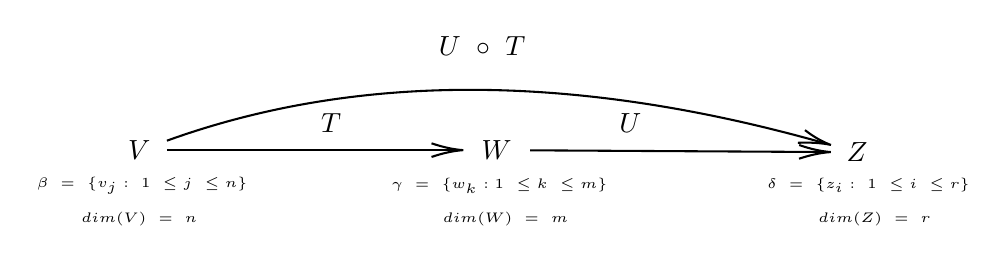
\begin{tikzpicture}[x=0.75pt,y=0.75pt,yscale=-1,xscale=1.4]
%uncomment if require: \path (0,235); %set diagram left start at 0, and has height of 235


% Text Node
\draw (123,131) node    {$V$};
% Text Node
\draw (246,131) node    {$W$};
% Text Node
\draw (370,132) node    {$Z$};
% Text Node
\draw (189,118) node    {$T$};
% Text Node
\draw (292,118) node    {$U$};
% Text Node
\draw (241,81) node    {$U\ \circ \ T$};
% Text Node
\draw (124,148) node  [font=\tiny]  {$\beta \ =\ \{v_{j} :\ 1\ \leq j\ \leq n \}$};
% Text Node
\draw (247,148) node  [font=\tiny]  {$\gamma \ =\ \{w_{k} :1\ \leq k\ \leq m \}$};
% Text Node
\draw (374,148) node  [font=\tiny]  {$\delta \ =\ \{z_{i} :\ 1\ \leq i\ \leq r\}$};
% Text Node
\draw (123,164) node  [font=\tiny]  {$dim( V) \ =\ n$};
% Text Node
\draw (249,164) node  [font=\tiny]  {$dim( W) \ =\ m$};
% Text Node
\draw (376,164) node  [font=\tiny]  {$dim( Z) \ =\ r$};
% Connection
\draw    (132.5,131) -- (232.5,131) ;
\draw [shift={(234.5,131)}, rotate = 180] [color={rgb, 255:red, 0; green, 0; blue, 0 }  ][line width=0.75]    (10.93,-3.29) .. controls (6.95,-1.4) and (3.31,-0.3) .. (0,0) .. controls (3.31,0.3) and (6.95,1.4) .. (10.93,3.29)   ;
% Connection
\draw    (257.5,131.09) -- (359,131.91) ;
\draw [shift={(361,131.93)}, rotate = 180.46] [color={rgb, 255:red, 0; green, 0; blue, 0 }  ][line width=0.75]    (10.93,-3.29) .. controls (6.95,-1.4) and (3.31,-0.3) .. (0,0) .. controls (3.31,0.3) and (6.95,1.4) .. (10.93,3.29)   ;
% Connection
\draw    (132.5,126.45) .. controls (198.12,93.27) and (273.85,93.77) .. (359.7,127.98) ;
\draw [shift={(361,128.49)}, rotate = 201.89] [color={rgb, 255:red, 0; green, 0; blue, 0 }  ][line width=0.75]    (10.93,-3.29) .. controls (6.95,-1.4) and (3.31,-0.3) .. (0,0) .. controls (3.31,0.3) and (6.95,1.4) .. (10.93,3.29)   ;

\end{tikzpicture}
\end{center}


Digamos pues que
\[
[U]_{\gamma}^{\delta} = 
\begin{pmatrix}
a_{11} & a_{12} & \ldots & a_{1m} \\
a_{21} & a_{22} & \ldots & a_{2m} \\
\vdots & \vdots & \ddots & \vdots \\
a_{r1} & a_{r2} & \ldots & a_{rm}
\end{pmatrix},
\hspace{0.2cm}
[T]_{\beta}^{\gamma} = 
\begin{pmatrix}
b_{11} & b_{12} & \ldots & b_{1n} \\
b_{21} & b_{22} & \ldots & b_{2n} \\
\vdots & \vdots & \ddots & \vdots \\
b_{k1} & b_{k2} & \ldots & b_{kn}
\end{pmatrix};
\]
estas dos ecuaciones matriciales equivalen a los siguientes
dos grupos de ecuaciones: 
\[
\forall 1 \leq j \leq n: \hspace{0.3cm}
T(v_{j}) = \sum_{k = 1}^{m} b_{kj} w_{k}
\]
y
\[
\forall 1 \leq k \leq m: \hspace{0.3cm}
U(w_{k}) = \sum_{i= 1}^{r} a_{ik} z_{i}.
\]

Ahora bien, la $j-$ésima columna de $[U \circ T]_{\beta}^{\delta}$
se consigue evaluando a $U \circ T$ en $v_{j}$:
\begin{align*}
(U \circ T)(v_{j}) = & U (T(v_{j})) = 
U\left( \sum_{k=1}^{m} b_{kj} w_{k} \right) \\
= & \sum_{k=1}^{m} b_{kj} U(w_{k}) = 
\sum_{k=1}^{m} b_{kj} \left( \sum_{i=1}^{r} a_{ik} z_{i} \right) \\
= & \sum_{i=1}^{r} \left( \sum_{k=1}^{m} a_{ik} b_{kj} \right) z_{i};
\end{align*}
reconociendo a $\sum_{k=1}^{m} a_{ik} b_{kj}$ como la $ij-$ésima
entrada del producto 
$[U]_{\gamma}^{\delta} \cdot  
[T]_{\beta}^{\gamma}$, terminamos.

\QEDB
\vspace{0.2cm}

\begin{lema}
	\label{lema: Ab como comb lineal de vectores col de A}
Sean $A = (a_{kj})_{\substack{ 1 \leq k \leq m \\ 1 \leq j \leq n }}
\in M_{m \times n} (F)$, $b = (b_{j})_{1 \leq j \leq n} \in M_{n \times 1}(F)$.
Si por $A_{., j}$ denotamos a la $j-$ésima columna de $A$, entonces
\marginnote{Nótese que la ecuación 
\eqref{eq: Ab como comb lineal de vectores col de A}
tiene sentido, pues tanto $Ab$ como los vectores columna de $A$ tienen
dimensión $m \times 1$.}
\begin{equation}
	\label{eq: Ab como comb lineal de vectores col de A}
	Ab = b_{1} A_{., 1} + \ldots + b_{n} A_{., n}, 
\end{equation}
es decir, $Ab$ es una combinación lineal de las columnas de $A$, 
donde los escalares de la combinación lineal son las entradas de $b$.
\end{lema}
\noindent
\textbf{Demostración.}
En efecto, la $k-$ésima entrada tanto de $Ab$ como de 
$\sum_{j = 1}^{n} A_{., j} b_{j}$
es $\sum_{j = 1}^{n}a_{kj}b_{j}$ ($k$ se mantiene fijo y se itera
el índice de columnas $j$ de $A$).

\begin{figure}[H]
\centering\captionsetup{format = hang}
		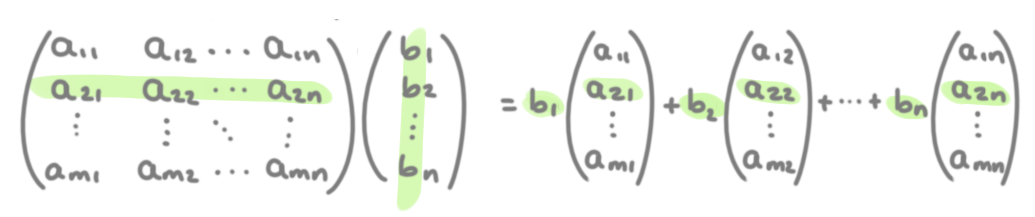
\includegraphics[scale=2.5]{21}
 \end{figure}
\QEDB 
\vspace{0.2cm}

\begin{teo}
	\label{teo: calculando Tx en terminos de representaciones matriciales}
Sean $V$ y $W$ dos $F-$espacios vectoriales finito dimensionales.
Si $\beta \subseteq V$ y $\gamma \subseteq W$ son bases de estos espacios
y $T: V \longrightarrow W$ es una transformación lineal, 
entonces, 
\[
\forall x \in V: \hspace{0.3cm} 
[T(x)]_{\gamma} = [T]_{\beta}^{\gamma} [x]_{\beta}.
\]
\end{teo}
\noindent
\textbf{Demostración.}
En efecto, 
si $\beta \ =\ \{v_{j} :\ 1\ \leq j\ \leq n \}$ y
\[
[x]_{\beta} = \begin{pmatrix}
x_{1} \\
\vdots \\
x_{n}
\end{pmatrix},
\hspace{0.2cm} \textit{ i.e. si }
x = \sum_{j=1}^{n} x_{i}v_{i},
\]
usando el Lema \ref{lema: Ab como comb lineal de vectores col de A},
se sigue de inmediato que 
\begin{align*}
[T]_{\beta}^{\gamma} = & 
x_{1} [T(v_{1})]_{\gamma} + x_{2} [T(v_{2})]_{\gamma} + \cdots + 
x_{n}[T(v_{n})]_{\gamma} \\
= & [x_{1}T(v_{1}) + \cdots + 
x_{n} T(v_{n})]_{\gamma} \\
= & [T(x_{1}v_{1} + \cdots + x_{n}v_{n})] = [T(x)]_{\gamma}.
\end{align*}

\QEDB
\vspace{0.2cm}


\hlgray{Ejercicio:} demuestra los siguientes resultados.
\begin{prop}
	Si $V$ es finito dimensional y 
	$\beta, \beta' \subseteq V$ son bases de $V$, entonces 
	\begin{itemize}
		\item $[Id]_{\beta}^{\beta'} = I_{n}$ si y sólo si $\beta$
		y $\beta'$ son iguales como bases ordenadas.
		\item La matriz $[Id]_{\beta}^{\beta'}$ es invertible, y 
		$$([Id]_{\beta}^{\beta'})^{-1} = [Id]_{\beta'}^{\beta}.$$
	\end{itemize}
\end{prop}


\section{Transformaciones lineales de la forma $L_{A}$}
Sea $A \in M_{m \times n} (F)$ una matriz de $m$ filas y 
$n$ columnas con coeficientes en $F$. Definimos a partir de ella
una transformación lineal como sigue:

\begin{equation}
	\label{eq: La}
L_{A} : F^{n} \longrightarrow F^{m}
\end{equation}
\[
L_{A}(x) = Ax,
\]
o sea, $L_{A}$ es la función ``multiplicar a $A$ por la izquierda
de vectores de $F^{n}$''.

Usando esta nueva notación, podemos establecer el Teorema
\ref{teo: calculando Tx en terminos de representaciones matriciales} en 
términos del siguiente diagrama de transformaciones lineales:
 
 \marginnote{Este diagrama representa lo explicado en el Teorema
 \ref{teo: calculando Tx en terminos de representaciones matriciales}.}
\begin{center}
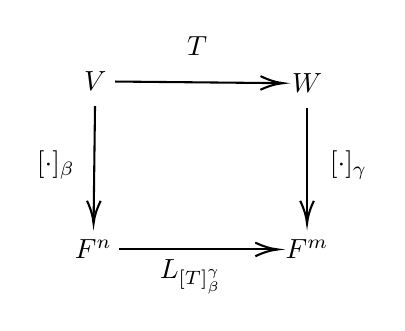
\begin{tikzpicture}[x=0.75pt,y=0.75pt,yscale=-1,xscale=1]
\draw (85,82.14) node    {$V$};
% Text Node
\draw (187,83.14) node    {$W$};
% Text Node
\draw (187,163.14) node    {$F^{m}$};
% Text Node
\draw (134,65.29) node    {$T$};
% Text Node
\draw (66,122.29) node    {$[ \cdot ]_{\beta }$};
% Text Node
\draw (84,163.14) node    {$F^{n}$};
% Text Node
\draw (207,122.29) node    {$[ \cdot ]_{\gamma }$};
% Text Node
\draw (131,176.29) node    {$L_{[T]_{\beta}^{\gamma}}$};
% Connection
\draw    (94.5,82.24) -- (173.5,83.01) ;
\draw [shift={(175.5,83.03)}, rotate = 180.56] [color={rgb, 255:red, 0; green, 0; blue, 0 }  ][line width=0.75]    (10.93,-3.29) .. controls (6.95,-1.4) and (3.31,-0.3) .. (0,0) .. controls (3.31,0.3) and (6.95,1.4) .. (10.93,3.29)   ;
% Connection
\draw  (187,95.14) -- (187,148.64) ;
\draw [shift={(187,150.64)}, rotate = 270] [color={rgb, 255:red, 0; green, 0; blue, 0 }  ][line width=0.75]    (10.93,-3.29) .. controls (6.95,-1.4) and (3.31,-0.3) .. (0,0) .. controls (3.31,0.3) and (6.95,1.4) .. (10.93,3.29)   ;
% Connection
\draw    (96.5,163.14) -- (171,163.14) ;
\draw [shift={(173,163.14)}, rotate = 180] [color={rgb, 255:red, 0; green, 0; blue, 0 }  ][line width=0.75]    (10.93,-3.29) .. controls (6.95,-1.4) and (3.31,-0.3) .. (0,0) .. controls (3.31,0.3) and (6.95,1.4) .. (10.93,3.29)   ;
% Connection
\draw    (84.85,94.14) -- (84.18,148.64) ;
\draw [shift={(84.15,150.64)}, rotate = 270.71] [color={rgb, 255:red, 0; green, 0; blue, 0 }  ][line width=0.75]    (10.93,-3.29) .. controls (6.95,-1.4) and (3.31,-0.3) .. (0,0) .. controls (3.31,0.3) and (6.95,1.4) .. (10.93,3.29)   ;
\end{tikzpicture}
\end{center}
Es decir,

\[
[\cdot]_{\gamma} \circ T = L_{[T]_{\beta}^{\gamma}} \circ [\cdot]_{\beta}.
\]

Nótese que partimos de espacios vectoriales $V$ y $W$ \textit{arbitrarios}
(siendo la única condición impuesta el que ambos sean finito dimensionales),
y que gracias a los isomorfismos $[\cdot]_{\beta}$ podemos 
usar transformaciones del tipo \eqref{eq: La} en lugar
de transformaciones $T: V \longrightarrow W$.

Algunas propiedades fáciles de probar sobre transformaciones
de la forma \eqref{eq: La} se enuncian y se dejan como ejercicio.
\begin{prop}
Si $L_{A}$ es como se definió en \eqref{eq: La}, entonces
\begin{itemize}
	\item $L_{A}$ es lineal
	\item Si $\beta$ y $\gamma$ son las bases canónicas de
	$F^{n}$ y $F^{m}$ respectivamente, entonces $[L_{A}]_{\beta}^{\gamma} = A$.
	\item $L_{A} = L_{B}$ si y sólo si $A = B$.
	\item $L_{A + B} = L_{A} + L_{B}$ y $L_{\lambda A} = \lambda L_{A}$
	para toda $\lambda \in F$.
	\item Si $T: F^{n} \longrightarrow F^{m}$ es una transformación lineal,
	entonces existe una única matriz $C$ de $m \times n$ tal que 
	$T = L_{C}$
	\item Si $E$ es una matriz de $n \times r$, entonces
	$L_{AE} = L_{A} \circ L_{E}$.
\end{itemize} 
\end{prop}

Veremos a continuación que la invertibilidad de 
una transformación lineal
$T$ (i.e. el que sea o no isomorfismo) está 
relacionada a la de cualquiera de sus representaciones matriciales
$[T]_{\beta}^{\gamma}$.

\marginnote{Recuerda que una matriz $A$ es invertible si y sólo si
$A$ es cuadrada y
existe $B$ otra matriz tal que $A B = I_{n} = B A$.}
\begin{teo}
Sea $T: V \longrightarrow W$ una transformación lineal entre dos
$F-$espacios vectoriales finito dimensionales $V$ y $W$.
Si $\beta \subseteq V$ y $\gamma \subseteq W$ son bases cualesquiera
de estos, entonces $T$ es un isomorfismo si y sólo si la matriz
$[T]_{\beta}^{\gamma}$ es invertible.
\end{teo}
\noindent
\textbf{Demostración.}
\begin{itemize}
	\item[$\Rightarrow$)] Supongamos que $T$ es un isomorfismo, es decir,
	que es invertible. Entonces, según la Proposición 
	\ref{prop: isomorfo implica misma dimension}, $dim(V) = dim(W)$.
	Sean $\beta = \{ v_{j}  | \hspace{0.2cm} 1 \leq j \leq n \}$ y
	$\gamma \{ w_{j}  | \hspace{0.2cm} 1 \leq j \leq n \}$ bases de $V$
	y $W$, y sea $T^{-1}: W \longrightarrow V$ la inversa de $T$ - que, 
	recuerde, también es una transformación lineal. Entonces, 
	según la proposición
	\ref{prop: calculo de composicion de transf a partir de producto de matr},
	\[
	I_{n} = [I_{V}]_{\beta}^{\beta} = [T^{-1} \circ T]_{\beta}^{\beta}
	= [T^{-1}]_{\gamma}^{\beta} [T]_{\beta}^{\gamma}
	\]
	y, análogamente,
	\[
	I_{n} = [T]_{\beta}^{\gamma} [T^{-1}]_{\gamma}^{\beta}.
	\]
	Así, $[T]_{\beta}^{\gamma}$ es invertible y, de hecho,
	\marginnote{La ecuación \eqref{eq: inversa de repr matr de T} es 
	importante en sí misma.}
	\begin{equation}
		\label{eq: inversa de repr matr de T}
		([T]_{\beta}^{\gamma})^{-1} = [T^{-1}]_{\gamma}^{\beta}.
	\end{equation}
	
	\item[$\Leftarrow$)] Sea $B \in M_{n \times n}(F)$ tal que
	\[
	[T]_{\beta}^{\gamma}B = I_{n} = B [T]_{\beta}^{\gamma}.
	\]
	Entonces, si $U: W \longrightarrow V$ es la única transformación lineal
	tal que $[U]_{\gamma}^{\beta} = B$, 
	\[
	[T \circ U]_{\gamma}^{\gamma} = [T]_{\beta}^{\gamma} [U]_{\gamma}^{\beta}
	= I_{n}.
	\]
	Esto implica que $T \circ U$ es la identidad en $W$. De forma
	análoga se prueba que $U \circ T$ es la identidad en $V$. Así,
	$T$ es invertible, luego, un isomorfismo.
\end{itemize}

\QEDB
\vspace{0.2cm}

\begin{prop}
Fijadas $\beta \subseteq V$ y $\gamma \subseteq W$ bases de los
$F-$espacios vectoriales finito dimensionales $V$ y $W$, 
la función 
\[
\Phi_{\beta}^{\gamma} : \mathcal{L}(V, W) \longrightarrow M_{m \times n}(F)
\]
\[
\Phi_{\beta}^{\gamma}(T) = [T]_{\beta}^{\gamma}.
\]
es un isomorfismo.
\end{prop}
\noindent
\textbf{Demostración.}
Ya vimos en proposciones anteriores la linealidad de 
$\Phi_{\beta}^{\gamma}$. 
\begin{itemize}
	\item Inyectividad: si $T: V \longrightarrow W$ es tal que
	$[T]_{\beta}^{\gamma}$ es la matriz cero, entonces $T$
	evaluada en cualquier vector de la base $\beta$ es cero, luego,
	$T$ debe ser la transformación lineal cero. Así,
	$Ker(\Phi_{\beta}^{\gamma}) = \{ 0 \}$.
	
	\item Suprayectividad: se estableció en la proposición 
	\ref{prop: suprayectividad de phi beta gamma}.
\end{itemize}

\QEDB
\vspace{0.2cm}

\section{Ejemplos}
Sea
\[
\mathcal{U}_{2}(\IR) = \left\{
\begin{pmatrix}
a & b \\
0 & c
\end{pmatrix}: \hspace{0.2cm}
a, b, c \in \IR
\right\} \leq M_{2 \times 2}
\]
el subespacio de matrices triangulares superiores de $2 \times 2$.
No es difícil convencerse de que este es un $\IR-$ espacio vectorial
de dimensión $3$, de hecho,
\[
\delta = \left\{
\begin{pmatrix}
1 & 0 \\
0 & 0
\end{pmatrix}, 
\begin{pmatrix}
0 & 1 \\
0 & 0
\end{pmatrix}, 
\begin{pmatrix}
0 & 0 \\
0 & 1
\end{pmatrix}
\right\}
\]
es una base para $\mathcal{U}_{2}(\IR)$.
Sean las transformaciones lineales
$S : \mathcal{U}_{2}(\IR) \longrightarrow \IR^{3}$,
$T: \mathbb{U}_{2}(\IR) \longrightarrow U_{2}(\IR)$
definidas como

\[
T \begin{pmatrix}
a & b \\
0 & c
\end{pmatrix} = 
\begin{pmatrix}
a & b \\
0 & a
\end{pmatrix} ,
\]
\[
U
\begin{pmatrix}
a & b \\
0 & c
\end{pmatrix} = 
(a, b, c)
\]
\hlpink{Terminar.}
\section{Cambio de sistema coordenado}


Ya ha quedado claro el uso de una base en un $F-$espacio 
vectorial $V$; estas actuan como un
\textbf{sistema de coordenadas}, pues, como se estableción
en el Teorema \ref{teo: equiv de base}
(resultado usado una y otra vez en el desarrollo
de la teoría anterior), si $\beta$ es base de $V$,
dado $x \in V$ \textit{cualquiera}, existen
\begin{itemize}
	\item \textbf{únicos} $v_{1}, \ldots, v_{n}$ de elementos 
	de $\beta$, y
	\item \textbf{únicos} escalares $a_{1}, \ldots, a_{n}$ escalares
	tales que
\end{itemize}
\[
x = \sum_{j = 1}^{n} a_{i} x_{i}.
\]
Recuerde que es por eso que, en el caso en el que $V$ es finito dimensional
(i.e. $\beta$ es finita), usamos esto para construir el isomorfismo
$[\cdot]_{\beta}$ entre $V$ y $F^{n}$ (justo asociándole a $x$ su única
colección de escalares $a_{1}, \ldots, a_{n}$). Note que esta representación
\textbf{depende de la base $\beta$}, es decir, si $\gamma \subseteq V$
es una base de $V$ distinta a $\beta$, entonces los isomorfismos
$[\cdot]_{\beta}$
y $[\cdot]_{\gamma}$ son distintos entre sí. Un caso particular de esta
situación es el realizar un cambio de coordenadas en el plano
(el espacio vectorial en esta situación es, por supuesto, $\IR^{2}$).

En este caso, ``fijar el plano/sistema coordenado'' y
``fijar la base'' significan lo mismo.
\TODO{Discusión del pizarrón. Fijar sistema de referencia, y usar nuevas
bases en ese sitema.}
\begin{ejem}
Mostremos cómo en ocasiones es conveniente cambiar de sistema de coordenadas.
En $\IR^{2}$, considere a la base canónica $\beta = \{ 
e_{1} = (1, 0), e_{2} = (0, 1) \}$.
Todo punto del espacio $(x, y)$ se expresa de forma única como combinación
lineal de elementos de $\beta$;
\[
(x, y) = x(1, 0) + y(0,1).
\]
Esta representación es muy sencilla - por eso resulta ventajoso en muchas
ocasiones trabajar con la base canónica de $\IR^{2}$. Considere al lugar 
geométrico $\mathcal{E} \subseteq \IR^{2}$ de puntos del plano que 
consta de los puntos que satisfacen la siguiente relación:
\begin{equation}
	\label{eq: elipse 1}
	w = (x, y) \in \mathcal{E} \hspace{0.2cm} \textit{ si y sólo si }
	\hspace{0.2cm}
	2x^{2} - 4xy + 5 y^{2} = 1.
\end{equation}
Puesto que en la ecuación para definir $\mathcal{E}$ están
involucrados cuadrados de las variables, parece que este lugar
geométrico es una cónica, sin embargo,
el término mixto $-4xy$ dificulta su identificación. Cambiemos 
de sistema coordenado; considérese a la base

\[
\beta' = \left\{
u = \left( \frac{\sqrt{5}}{5}, -\frac{2 \sqrt{5}}{5} \right),
v = \left( \frac{2\sqrt{5}}{5}, \frac{\sqrt{5}}{5} \right)
\right\}.
\]
Si $w = (x, y) \in \IR^{2}$, entonces
\begin{align*}
w = (x, y) = & x e_{1} + y e_{2} \\
= & x'u + y' v \\
= &  x' \left( \frac{\sqrt{5}}{5}, -\frac{2 \sqrt{5}}{5} \right) 
+ y' \left( \frac{2\sqrt{5}}{5}, \frac{\sqrt{5}}{5} \right) \\
= &x' \left( \frac{\sqrt{5}}{5} e_{1} -
\frac{2\sqrt{5}}{5} e_{2} \right)
+ y' \left( \frac{2\sqrt{5}}{5}e_{1} + 
\frac{\sqrt{5}}{5} e_{2} \right) \\
= & \left( \frac{\sqrt{5}}{5} x' + \frac{2\sqrt{5}}{5} y' \right)e_{1} + 
\left( -\frac{2\sqrt{5}}{5} x' + \frac{\sqrt{5}}{5}y' \right) e_{2}.
\end{align*}

\marginnote{A esta situación se le conoce en geometría analítica como
``eliminación del término mixto''.}

De la igualdad de los coeficientes al representar vectores respecto a una
base se deduce que 
\begin{equation}
	\label{eq: relacion x x' cambio base ejemplo}
	x = \frac{\sqrt{5}}{5} x' + \frac{2\sqrt{5}}{5} y', 
	\hspace{0.2cm}
	y =  -\frac{2\sqrt{5}}{5} x' + \frac{\sqrt{5}}{5}y'.
\end{equation}
Si usamos ahora el sistema coordenado $\beta'$, debemos sustituir 
los cambios \eqref{eq: relacion x x' cambio base ejemplo}
en la condición de definición \eqref{eq: elipse 1}. Haciendo esto, 
llegamos a que 
\begin{equation}
	\label{eq: elipse 2}
	w = x'u + y'v \in \mathcal{E} 
	\hspace{0.2cm} \textit{ si y sólo si }
	\hspace{0.2cm}
	6(x')^{2} + (y')^{2} = 1.
\end{equation}
Ahora sí reconocemos al lugar geométrico como una elipse, pero 
\textbf{no} respecto al sistema coordenado $\beta$, sino respecto 
a $\beta'$.
\begin{marginfigure}
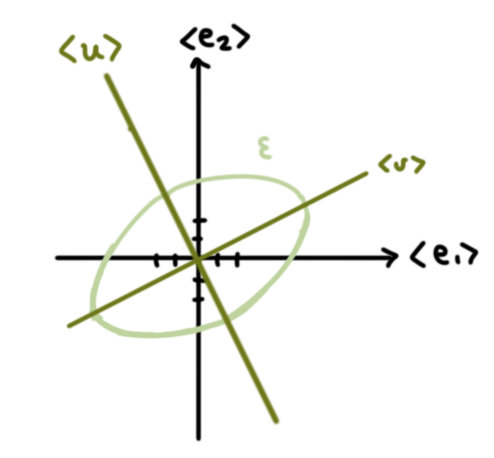
\includegraphics[scale= 2.3]{22}
\end{marginfigure}

Al dibujar el nuevo sistema coordenado en el plano (i.e. a las 
rectas $\langle \{ u \} \rangle$ y $\langle \{ v \} \rangle$, que son 
subespacios uno dimensionales de $\IR^{2}$), notamos que este se 
obtiene rotando el sistema original $\beta$.

Observa que la relación 
\eqref{eq: relacion x x' cambio base ejemplo}
(que nos permitió pasar de una base a otra) puede representarse
en forma matricial como 
\[
\begin{pmatrix}
x \\ y
\end{pmatrix} = 
\begin{pmatrix}
\frac{\sqrt{5}}{5} & \frac{2\sqrt{5}}{5} \\
-\frac{2\sqrt{5}}{5} & \frac{\sqrt{5}}{5}
\end{pmatrix}
\begin{pmatrix}
x' \\ y'
\end{pmatrix};
\]
nota que 
\[
[w]_{\beta} = \begin{pmatrix}
x \\ y
\end{pmatrix},
\hspace{0.2cm}
[Id]_{\beta'}^{\beta} = 
\begin{pmatrix}
\frac{\sqrt{5}}{5} & \frac{2\sqrt{5}}{5} \\
-\frac{2\sqrt{5}}{5} & \frac{\sqrt{5}}{5}
\end{pmatrix},
\hspace{0.2cm}
[w]_{\beta'} = \begin{pmatrix}
x' \\ y'
\end{pmatrix}.
\]
\end{ejem}

Usando el que la transformación lineal identidad es el neutro de
la composición y que multiplicación de matrices es la operación 
correspondiente a composición de funciones, se establece fácilmente
cómo hacer cambios de base.

\begin{teo}
Sean $\beta$, $\beta'$ dos bases de un $F-$espacio vectorial finito 
dimensional $V$. Sea $Q = [Id_{V}]_{\beta'}^{\beta}$.
\begin{itemize}
	\item La matriz $Q$ es invertible.
	\item Para toda $v \in V$,
	\begin{equation}
		\label{eq: v beta igual a id por v beta prima}
		[v]_{\beta} = Q [v]_{\beta'}.
	\end{equation}
\end{itemize}
\end{teo}
\marginnote{La ecuación \eqref{eq: v beta igual a id por v beta prima}
nos explica cómo obtener las coordenadas de un vector $v$
en términos de $\beta$ cuando se tienen sus coordenadas en 
términos de $\beta'$.}
\noindent
\textbf{Demostración.}
Claro que $Q$ es invertible, pues la transformación identidad
$Id_{V}$ es un isomorfismo (c.f. \TODO{cita}).
Además, según 
el Teorema \ref{teo: calculando Tx en terminos de representaciones matriciales},
\[
[v]_{\beta} = [Id_{V}(v)]_{\beta} = [Id]_{\beta'}^{\beta}[v]_{\beta'}.
\]
\QEDB
\vspace{0.2cm}

\begin{defi}
Si $\beta$ y $\beta'$ son dos bases de un $F-$espacio vectorial
finito dimensional $V$, a la matriz $[Id]_{\beta'}^{\beta}$
se le conoce como \textbf{matriz de cambio de base} de 
$\beta'$ a $\beta$.
\end{defi}

\TODO{Poner ejemplo numérico.}

Sean $V$ y $W$ dos $F-$espacios vectoriales, y considere dos pares de bases
\[
\beta \subseteq V, \gamma \subseteq W;
\hspace{0.4cm}
\beta' \subseteq V, \gamma' \subseteq W
\]
de estos.
Dada una transformación lineal $T: V \longrightarrow W$,
según el Teorema 
\ref{teo: calculando Tx en terminos de representaciones matriciales},
tenemos los siguientes dos cuadrados conmutativos;
\begin{center}
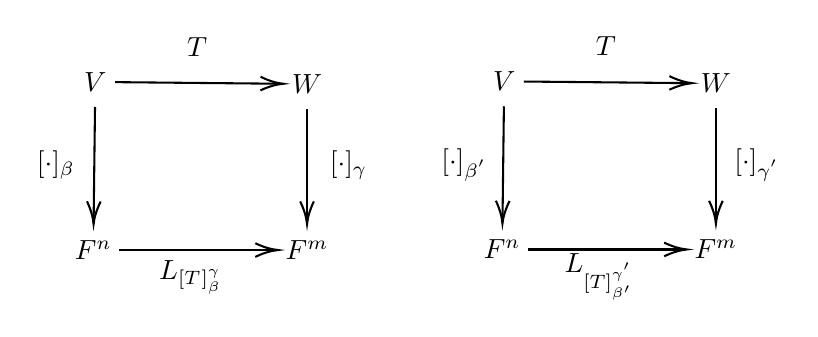
\begin{tikzpicture}[x=0.75pt,y=0.75pt,yscale=-1,xscale=1]
%uncomment if require: \path (0,235); %set diagram left start at 0, and has height of 235


% Text Node
\draw (85,82.14) node    {$V$};
% Text Node
\draw (187,83.14) node    {$W$};
% Text Node
\draw (187,163.14) node    {$F^{m}$};
% Text Node
\draw (134,65.29) node    {$T$};
% Text Node
\draw (66,122.29) node    {$[ \cdot ]_{\beta }$};
% Text Node
\draw (84,163.14) node    {$F^{n}$};
% Text Node
\draw (207,122.29) node    {$[ \cdot ]_{\gamma }$};
% Text Node
\draw (131,176.29) node    {$L_{[ T}{}_{]_{\beta }^{\gamma }}$};
% Text Node
\draw (282,81.86) node    {$V$};
% Text Node
\draw (384,82.86) node    {$W$};
% Text Node
\draw (384,162.86) node    {$F^{m}$};
% Text Node
\draw (331,65) node    {$T$};
% Text Node
\draw (263,122) node    {$[ \cdot ]_{\beta ^{'}}$};
% Text Node
\draw (281,162.86) node    {$F^{n}$};
% Text Node
\draw (404,122) node    {$[ \cdot ]_{\gamma ^{'}}$};
% Text Node
\draw (328,176) node    {$L_{[T]_{\beta'}^{\gamma^{'}}}$};
% Connection
\draw    (94.5,82.24) -- (173.5,83.01) ;
\draw [shift={(175.5,83.03)}, rotate = 180.56] [color={rgb, 255:red, 0; green, 0; blue, 0 }  ][line width=0.75]    (10.93,-3.29) .. controls (6.95,-1.4) and (3.31,-0.3) .. (0,0) .. controls (3.31,0.3) and (6.95,1.4) .. (10.93,3.29)   ;
% Connection
\draw (187,95.14) -- (187,148.64) ;
\draw [shift={(187,150.64)}, rotate = 270] [color={rgb, 255:red, 0; green, 0; blue, 0 }  ][line width=0.75]    (10.93,-3.29) .. controls (6.95,-1.4) and (3.31,-0.3) .. (0,0) .. controls (3.31,0.3) and (6.95,1.4) .. (10.93,3.29)   ;
% Connection
\draw    (96.5,163.14) -- (171,163.14) ;
\draw [shift={(173,163.14)}, rotate = 180] [color={rgb, 255:red, 0; green, 0; blue, 0 }  ][line width=0.75]    (10.93,-3.29) .. controls (6.95,-1.4) and (3.31,-0.3) .. (0,0) .. controls (3.31,0.3) and (6.95,1.4) .. (10.93,3.29)   ;
% Connection
\draw    (84.85,94.14) -- (84.18,148.64) ;
\draw [shift={(84.15,150.64)}, rotate = 270.71] [color={rgb, 255:red, 0; green, 0; blue, 0 }  ][line width=0.75]    (10.93,-3.29) .. controls (6.95,-1.4) and (3.31,-0.3) .. (0,0) .. controls (3.31,0.3) and (6.95,1.4) .. (10.93,3.29)   ;
% Connection
\draw    (291.5,81.95) -- (370.5,82.72) ;
\draw [shift={(372.5,82.74)}, rotate = 180.56] [color={rgb, 255:red, 0; green, 0; blue, 0 }  ][line width=0.75]    (10.93,-3.29) .. controls (6.95,-1.4) and (3.31,-0.3) .. (0,0) .. controls (3.31,0.3) and (6.95,1.4) .. (10.93,3.29)   ;
% Connection
\draw  (384,94.86) -- (384,148.36) ;
\draw [shift={(384,150.36)}, rotate = 270] [color={rgb, 255:red, 0; green, 0; blue, 0 }  ][line width=0.75]    (10.93,-3.29) .. controls (6.95,-1.4) and (3.31,-0.3) .. (0,0) .. controls (3.31,0.3) and (6.95,1.4) .. (10.93,3.29)   ;
% Connection
\draw    (293.5,162.86) -- (368,162.86) ;
\draw [shift={(370,162.86)}, rotate = 180] [color={rgb, 255:red, 0; green, 0; blue, 0 }  ][line width=0.75]    (10.93,-3.29) .. controls (6.95,-1.4) and (3.31,-0.3) .. (0,0) .. controls (3.31,0.3) and (6.95,1.4) .. (10.93,3.29)   ;
% Connection
\draw    (281.85,93.86) -- (281.18,148.36) ;
\draw [shift={(281.15,150.36)}, rotate = 270.71] [color={rgb, 255:red, 0; green, 0; blue, 0 }  ][line width=0.75]    (10.93,-3.29) .. controls (6.95,-1.4) and (3.31,-0.3) .. (0,0) .. controls (3.31,0.3) and (6.95,1.4) .. (10.93,3.29)   ;

\end{tikzpicture}
\end{center}
Ambos diagramas hacen referencia a $T$ (su objetivo de hecho es 
decir cómo
evaluar a $T$ en vectores de $V$ en términos de multiplicaciones
de matrices). ¿Qué relación hay entre estos? En otras palabras,
¿Cómo conociendo la representación matricial 
$[T]_{\beta}^{\gamma}$ encontramos a $[T]_{\beta'}^{\gamma'}$?
\begin{center}
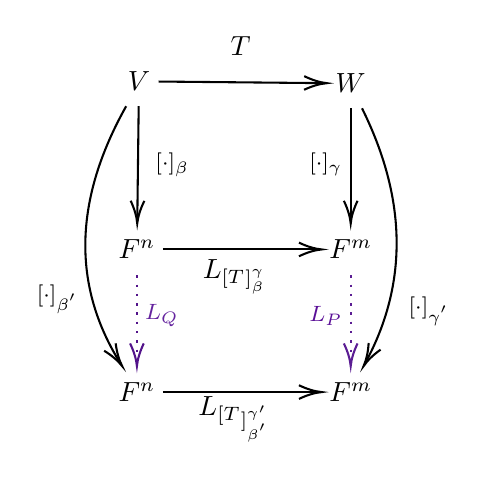
\begin{tikzpicture}[x=0.75pt,y=0.75pt,yscale=-1,xscale=1]
%uncomment if require: \path (0,235); %set diagram left start at 0, and has height of 235


% Text Node
\draw (87,27.14) node    {$V$};
% Text Node
\draw (189,28.14) node    {$W$};
% Text Node
\draw (189,108.14) node    {$F^{m}$};
% Text Node
\draw (136,10.29) node    {$T$};
% Text Node
\draw (103,67.29) node  [font=\footnotesize]  {$[ \cdot ]_{\beta }$};
% Text Node
\draw (86,108.14) node  [color={rgb, 255:red, 0; green, 0; blue, 0 }  ,opacity=1 ]  {$F^{n}$};
% Text Node
\draw (177,67.29) node  [font=\footnotesize]  {$[ \cdot ]_{\gamma }$};
% Text Node
\draw (133,121.29) node    {$L_{[ T}{}_{]_{\beta }^{\gamma }}$};
% Text Node
\draw (189,176.86) node    {$F^{m}$};
% Text Node
\draw (86,176.86) node    {$F^{n}$};
% Text Node
\draw (133,190) node    {$L_{[ T}{}_{]_{\beta ^{'}}^{\gamma '}}$};
% Text Node
\draw (48,132) node  [font=\footnotesize]  {$[ \cdot ]_{\beta ^{'}}$};
% Text Node
\draw (227,138) node  [font=\footnotesize]  {$[ \cdot ]_{\gamma ^{'}}$};
% Text Node
\draw (98,140.14) node  [font=\footnotesize,color={rgb, 255:red, 100; green, 35; blue, 158 }  ,opacity=1 ]  {$L_{Q}$};
% Text Node
\draw (177,140.14) node  [font=\footnotesize,color={rgb, 255:red, 90; green, 15; blue, 151 }  ,opacity=1 ]  {$L_{P}$};
% Connection
\draw    (96.5,27.24) -- (175.5,28.01) ;
\draw [shift={(177.5,28.03)}, rotate = 180.56] [color={rgb, 255:red, 0; green, 0; blue, 0 }  ][line width=0.75]    (10.93,-3.29) .. controls (6.95,-1.4) and (3.31,-0.3) .. (0,0) .. controls (3.31,0.3) and (6.95,1.4) .. (10.93,3.29)   ;
% Connection
\draw    (189,40.14) -- (189,93.64) ;
\draw [shift={(189,95.64)}, rotate = 270] [color={rgb, 255:red, 0; green, 0; blue, 0 }  ][line width=0.75]    (10.93,-3.29) .. controls (6.95,-1.4) and (3.31,-0.3) .. (0,0) .. controls (3.31,0.3) and (6.95,1.4) .. (10.93,3.29)   ;
% Connection
\draw    (98.5,108.14) -- (173,108.14) ;
\draw [shift={(175,108.14)}, rotate = 180] [color={rgb, 255:red, 0; green, 0; blue, 0 }  ][line width=0.75]    (10.93,-3.29) .. controls (6.95,-1.4) and (3.31,-0.3) .. (0,0) .. controls (3.31,0.3) and (6.95,1.4) .. (10.93,3.29)   ;
% Connection
\draw    (86.85,39.14) -- (86.18,93.64) ;
\draw [shift={(86.15,95.64)}, rotate = 270.71] [color={rgb, 255:red, 0; green, 0; blue, 0 }  ][line width=0.75]    (10.93,-3.29) .. controls (6.95,-1.4) and (3.31,-0.3) .. (0,0) .. controls (3.31,0.3) and (6.95,1.4) .. (10.93,3.29)   ;
% Connection
\draw    (98.5,176.86) -- (173,176.86) ;
\draw [shift={(175,176.86)}, rotate = 180] [color={rgb, 255:red, 0; green, 0; blue, 0 }  ][line width=0.75]    (10.93,-3.29) .. controls (6.95,-1.4) and (3.31,-0.3) .. (0,0) .. controls (3.31,0.3) and (6.95,1.4) .. (10.93,3.29)   ;
% Connection
\draw    (80.81,39.14) .. controls (55.48,84.3) and (54.61,125.66) .. (78.18,163.22) ;
\draw [shift={(78.9,164.36)}, rotate = 237.29] [color={rgb, 255:red, 0; green, 0; blue, 0 }  ][line width=0.75]    (10.93,-3.29) .. controls (6.95,-1.4) and (3.31,-0.3) .. (0,0) .. controls (3.31,0.3) and (6.95,1.4) .. (10.93,3.29)   ;
% Connection
\draw    (194.45,40.14) .. controls (216.1,83.77) and (216.67,124.59) .. (196.15,162.62) ;
\draw [shift={(195.2,164.36)}, rotate = 299.15] [color={rgb, 255:red, 0; green, 0; blue, 0 }  ][line width=0.75]    (10.93,-3.29) .. controls (6.95,-1.4) and (3.31,-0.3) .. (0,0) .. controls (3.31,0.3) and (6.95,1.4) .. (10.93,3.29)   ;
% Connection
\draw [color={rgb, 255:red, 82; green, 19; blue, 138 }  ,draw opacity=1 ] [dash pattern={on 0.84pt off 2.51pt}]  (86,120.64) -- (86,162.36) ;
\draw [shift={(86,164.36)}, rotate = 270] [color={rgb, 255:red, 82; green, 19; blue, 138 }  ,draw opacity=1 ][line width=0.75]    (10.93,-3.29) .. controls (6.95,-1.4) and (3.31,-0.3) .. (0,0) .. controls (3.31,0.3) and (6.95,1.4) .. (10.93,3.29)   ;
% Connection
\draw [color={rgb, 255:red, 91; green, 29; blue, 147 }  ,draw opacity=1 ] [dash pattern={on 0.84pt off 2.51pt}]  (189,120.64) -- (189,162.36) ;
\draw [shift={(189,164.36)}, rotate = 270] [color={rgb, 255:red, 91; green, 29; blue, 147 }  ,draw opacity=1 ][line width=0.75]    (10.93,-3.29) .. controls (6.95,-1.4) and (3.31,-0.3) .. (0,0) .. controls (3.31,0.3) and (6.95,1.4) .. (10.93,3.29)   ;

\end{tikzpicture}
\end{center}
Podemos usar matrices de cambio de base para pasar fácilmente de una
representación matricial a la otra. En efecto, 
si 
\[
P = [Id_{W}]_{\gamma}^{\gamma'}, \hspace{0.2cm}
Q = [Id_{V}]_{\beta}^{\beta'}, 
\]
entonces,
para toda $v \in V$,
$$P[T]_{\beta}^{\gamma} [v]_{\beta} = ([Id_{W}]_{\gamma}^{\gamma'}
	[T]_{\beta}^{\gamma})[v_{\beta}] = [Id_{W} \circ T]_{\beta}^{\gamma'}
	[v]_{\beta} = [T]_{\beta}^{\gamma'}[v]_{\beta} = [T(v)]_{\gamma},$$
y también
$$
[T]_{\beta'}^{\gamma'} Q [v]_{\beta} = ([T]_{\beta'}^{\gamma'}
[Id_{V}]_{\beta}^{\beta'})[v]_{\beta} = [T \circ Id_{V}]_{\beta}^{\gamma'}
[v]_{\beta} = [T]_{\beta}^{\gamma'}[v]_{\beta} = [T(v)]_{\gamma}.
$$
De esto se deduce que 
\begin{equation}
	\label{eq: P T beta gama = T beta' gamma' Q}
	P[T]_{\beta}^{\gamma} = [T]_{\beta'}^{\gamma'} Q.
\end{equation}
\marginnote{En efecto, toma a $[v]_{\beta}$ como un vector de la base 
canónica de $F^{n}$ para probar que las correspondientes columnas de 
las matrices en \eqref{eq: P T beta gama = T beta' gamma' Q} en
efecto coinciden entre sí.}
Puesto que $P$ es invertible, podemos despejar a $[T]_{\beta}^{\gamma}$
de \eqref{eq: P T beta gama = T beta' gamma' Q}.
Hemos demostrado así el siguiente 
\begin{teo}
	\label{teo: cambio de bases repr matr}
Sean $V$ y $W$ dos $F-$espacios vectoriales finito dimensionales,
$T: V \longrightarrow W$ una transformación lineal entre ellos.
Si $\beta, \beta' \subseteq V$ y $\gamma, \gamma' \subseteq W$ son 
bases para estos espacios, 
\begin{itemize}
	\item $P = [Id_{W}]_{\gamma}^{\gamma'}$ es la matriz que transforma
	las coordenadas de $\gamma$ en $\gamma'$, y 
	\item $Q = [Id_{V}]_{\beta}^{\beta'}$ es la matriz que transforma
	las coordenadas de $\beta$ en $\beta'$,
\end{itemize}
entonces,
\begin{equation}
	\label{eq: T beta gama = P inv T beta' gamma' Q}
	[T]_{\beta}^{\gamma} = P^{-1} [T]_{\beta'}^{\gamma'} Q.
\end{equation}
\end{teo}

\begin{obs}
Si $V$ es un $F-$espacio vectorial finito dimensional y 
$\beta, \beta' \subseteq V$ son bases de $V$, entonces
\begin{equation}
	\label{eq: inversa de id beta a beta' es con bases en otro orden}
	([Id_{V}]_{\beta}^{\beta'})^{-1} = [Id_{V}]_{\beta'}^{\beta}.
\end{equation}
\end{obs}

\TODO{Ejemplo numérico con observaciones.}

Vale la pena escribir el Teorema 
\ref{teo: cambio de bases repr matr} para el caso particular 
en el que el espacio de dominio coincide con el de codominio.

\begin{cor}
	\label{cor: T de V en V cambio de base}
Si $V$ es un $F-$espacio vectorial finito dimensional y 
$\beta, \beta' \subseteq V$ son bases de $V$, entonces
\begin{equation}
	\label{eq: T de V en V dos bases}
	[T]_{\beta}^{\beta} = Q^{-1} [T]_{\beta'}^{\beta'} Q,
\end{equation}
donde $Q= [Id_{V}]_{\beta}^{\beta'}$.
\end{cor}

\subsection{Matrices similares}
\TODO{Sigue discusión y salta a 
p. 239 Friedb.}

\begin{defi}
	\label{def: matrices similares}
Sean $A, B \in M_{n \times n}(F)$. Decimos que las matrices $A$ y $B$
son \textbf{similares} si existe $Q \in M_{n \times n}(F)$ invertible tal que
\[
A = Q^{-1}B Q.
\]
\end{defi}
En términos de esta definición, el Corolario 
\ref{cor: T de V en V cambio de base} se resume como sigue:
\begin{center}
\textit{Las representaciones matriciales de una transformación lineal
$T: V \longrightarrow V$ respecto a una misma base son todas similares entre
sí.}
\end{center}
No es difícil demostrar que la relación ``ser similar con''
es de equivalencia:

\noindent
\hlgray{Ejercicio:} Demuestra que la relación en el conjunto
de las matrices cuadradas $n \times n$ dada por
\begin{equation}
	\label{eq: relacion equiv ser similar a}
\forall A, B \in M_{n \times n}(F): \hspace{0.2cm}
A \sim B \hspace{0.2cm} \Leftrightarrow
\exists Q \in M_{n \times n}(F) \textit{ invertible tal que }
A = Q^{-1}B Q
\end{equation}
es de equivalencia, es decir, que 
\begin{itemize}
	\item es reflexiva: $\forall A \in M_{n \times n}(F): A \sim A$,
	\item simétrica: $\forall A, B \in M_{n \times n}(F): A \sim B
	\Rightarrow B \sim A$, y
	\item transitiva: $\forall A, B, C \in M_{n \times n}(F):
	A \sim B \wedge B \sim C \Rightarrow A \sim C$.
\end{itemize}

Como toda relación de equivalencia
en el conjunto $M_{n \times n}(F)$.
esta induce una partición
en él. 

\begin{notacion}
	Si $A \in M_{n \times n}(F)$, por $\overline{A}$
	denotaremos a la clase de equivalencia de $A$ bajo la relación
	``ser similar a'';
	\[
	\overline{A} = \{ B \in M_{n \times n}(F) : \hspace{0.2cm} 
	A \sim B
	\}.
	\]
\end{notacion}


\begin{marginfigure}
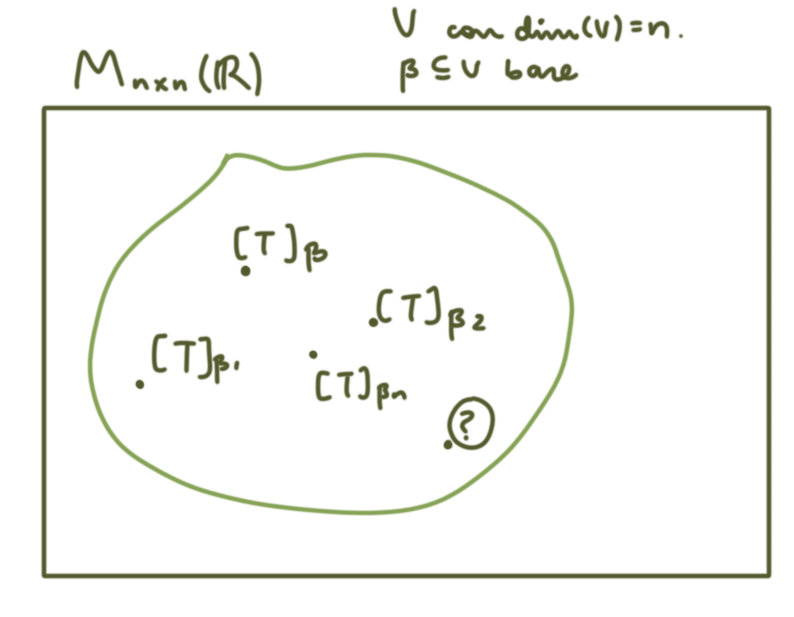
\includegraphics[scale= 1.5]{23} 
		\caption{ }
\end{marginfigure}

Sea $V$ un $F-$espacio vectorial
con $dim(V) = n$ (por ejemplo, $V = F^{n}$).
Si $T: V \longrightarrow V$ es una transformación lineal y 
$\beta \subseteq V$ es una base para $V$, consideremos a la
matriz $A = [T]_{\beta}^{\beta}$. 
Según el Corolario \ref{cor: T de V en V cambio de base},
si $\beta' \subseteq V$ es otra base cualquiera de $V$,
\begin{align*}
	[T]_{\beta'}^{\beta'} = Q^{-1} [T]_{\beta}^{\beta} Q = 
	Q^{-1} A Q,
\end{align*}
donde $Q = [Id_{V}]_{\beta'}^{\beta}$ es en efecto invertible
(pues $Id_{V}: V \longrightarrow V$ lo es).
Esto significa que 
\[
\{
[T]_{\beta'}^{\beta'} : \hspace{0.2cm} \beta' \subseteq V
\hspace{0.1cm} \textit{ es base }
\} \subseteq \overline{A}.
\]
¿Se tiene también la otra inclusión?
Damos una respuesta afirmativa en el siguiente

\begin{teo}
	\label{teo: similar a repr matricial de T sii tambien es repr matr de T}
	Sea $V$ un $F-$espacio vectorial $n-$dimensional, $T: V \longrightarrow V$
	lineal. Si $$\beta = \{ v_{1}, \ldots , v_{n} \}
	\subseteq V$$ es base y $A = [T]_{\beta}^{\beta}$, 
	entonces,
	\[
	\forall B \in M_{n \times n}(F): \hspace{0.2cm} A \sim B \hspace{0.2cm}
	\textit{si y sólo si existe } \beta' \subseteq V \textit{ base 
	tal que } B = [T]_{\beta'}^{\beta'}.
	\]
	Es decir, la clase de equivalencia de $A = [T]_{\beta}^{\beta}$
	bajo la relación de equivalencia 
	\eqref{eq: relacion equiv ser similar a} es
	\[
	\{ [T]_{\beta'}^{\beta'}  | \hspace{0.2cm} \beta' \subseteq V \textit{ 
	es base} \}.
	\]
\end{teo}
\noindent
\textbf{Demostración.}
Sea $B \in M_{n \times n}(F)$ similar a $A$; digamos pues que 
$Q \in M_{n \times n}(F)$ es una matriz invertible tal que 
\begin{equation}
	\label{eq: B q menos uno a q}
	B = Q^{-1} A Q = Q^{-1} [T]_{\beta}^{\beta} Q. 
\end{equation} 
Usando la matriz $Q$ vamos a construir una base para $V$; 
definamos a los vectores

\begin{equation}
	\label{eq: vj prima a partir de base y matr invertible Q}
	v_{j}' := q_{1j} v_{1} + q_{2j}v_{2} + \cdots + q_{nj} v_{n}, 
	\hspace{0.2cm} 1 \leq j \leq n.
\end{equation}
O sea, tomamos a las columnas de $Q$ como listas de coeficientes.
Sea $\beta' = \{v_{1}', \ldots , v_{n}' \}$.
Si $a_{1}, \ldots , a_{n} \in F$ tales que 
\begin{align*}
	0 = & a_{1}v_{1}' + \cdots + a_{n}v_{n}' \\
	= & a_{1}(q_{11}v_{1} + \cdots + p_{n1}v_{n}) + \cdots +
	a_{n}(q_{1n}v_{1} + \cdots + p_{nn}v_{n}) \\
	= & (a_{1}p_{11} + \cdots a_{n}p_{1n}) v_{1} + \cdots +
	(a_{1}p_{n1} + \cdots a_{n}p_{nn}) v_{n},
\end{align*}
luego, como $\beta$ es l.i., tenemos que los coeficientes de
la combinación lineal anterior son todos cero, hecho que puede
reescribirse como la siguiente ecuación matricial;
\[
Q a = 0_{F^{n}}, \hspace{0.2cm}
a := \begin{pmatrix}
	a_{1} \\
	\vdots \\
	a_{n}
\end{pmatrix}.
\]
Por ser $Q$ invertible, de esta última igualdad se deduce que 
$a$ es el vector cero de $F^{n}$. De esto se concluye que 
$\beta'$ es l.i., luego, como tiene cardinalidad $n$
(el que sea l.i. implica que los vectores $v_{j}'$ son 
distintos entre sí), es base de $V$. La definición 
\eqref{eq: vj prima a partir de base y matr invertible Q} de 
los vectores $v_{i}'$ se reinterpreta ahora como
\begin{equation}
	\label{eq: Q es id de beta prima a beta.}
	Q = [Id]_{\beta'}^{\beta}.
\end{equation}
Sustituyendo a \eqref{eq: Q es id de beta prima a beta.} en 
\eqref{eq: B q menos uno a q}, concluimos que 
\begin{align*}
	B = [Id]_{\beta}^{\beta'} [T]_{\beta}^{\beta} [Id]_{\beta'}^{\beta}
	= [T]_{\beta'}^{\beta'}.
\end{align*}

\QEDB
\vspace{0.2cm}


\section{Cálculo del rango de transformaciones usando representaciones matriciales}

\begin{defi}
Sea $A \in M_{m \times n}(F)$ una matriz. Definimos su \textbf{rango}
como la máxima cantidad de columnas linealmente independientes que tenga.
\end{defi}

Recuerda que el rango de una transformación
lineal $T: V \longrightarrow W$ se definió como la dimensión de
su imagen.

\begin{prop}
El rango columna es igual al rango fila. \hlpink{Reformular y demostrar.}
\end{prop}

\begin{prop}
	\label{prop: rango de matriz A coincide con rango de transf LA}
Si $A \in M_{m \times n}(F)$, entonces su rango coincide con el rango
de su transformación lineal asociada, o sea, 
\begin{equation}
	\label{eq: rango de matriz usando su transformacion lineal}
	Rango(A) = dim(L_{A}(F^{n})).
\end{equation}
\end{prop}
\noindent
\textbf{Demostración.}
Si $e_{i}$ es el $i-$ésimo vector de la base canónica de $F^{n}$, 
note que $L_{A}(e_{i}) = Ae_{i}$ es la $i-$ésima columna de $A$.
Además, como $\{ e_{1}, \ldots, e_{n} \}$ es base de
$F^{n}$, $\{ L_{A}(e_{1}), \ldots, L_{A}(e_{n}) \}$
genera a $L_{A}(F^{n})$ (c.f. Corolario
\ref{cor: imagen de base de V bajo lineal genera a W}). Es decir,
los vectores columna generan al espacio imagen de $L_{A}$; extraer
de este generador una base es lo mismo que encontrar la mayor
cantidad de columnas linealmente independientes de $A$.

\QEDB
\vspace{0.2cm}

\begin{prop}
	\label{prop: isomorfismos respetan dimension de subespacios}
Si $V$ es finito dimensional y $U: V \longrightarrow W$ es un isomorfismo,
entonces, para todo $X \leq V$, $dim(X) = dim(U(X))$.
\end{prop}
\noindent
\textbf{Demostración.}
Claro que la restricción
$U_{|X}: X \longrightarrow U(X)$ es, por herencia de $U$,
lineal e inyectiva, y por como hemos definido el codominio, también
es suprayectiva, luego, es un isomorfismo, por lo tanto, 
según la proposición 
\ref{prop: isomorfo implica misma dimension}, 
$dim(X) = dim(U(X))$.
\QEDB
\vspace{0.2cm}


\begin{prop}
Sea $V$ finito dimensional, $T: V \longrightarrow W$ lineal. 
Si $U: Z \longrightarrow V$ es un isomorfismo, entonces
\[
dim(Ker(T \circ U)) = dim(Ker(T)), 
\hspace{0.2cm} dim(T\circ U (Z)) = dim(T (V)),
\]
es decir, componer por la derecha con un isomorfismo no altera
la dimensión del Kernel o de la imagen de una transformación lineal.
\end{prop}
\noindent
\textbf{Demostración.}
\marginnote{Nota que, como $U$ es invertible, aquí $U^{-1}(C)$ es la
imagen bajo $C$ de la transformación inversa $U^{-1}$.}
Como $U$ es un isomorfismo, $dim(Z) = dim(V)$.
Obsérvese que $x \in Ker(T \circ U)$ si y sólo si 
$T(U(x)) = 0$, o sea, si y sólo si $U(x) \in Ker(T)$, entonces,
\[
Ker(T \circ U) = U^{-1}(Ker(T)).
\]
Además, $U^{-1}$ es un isomorfismo, luego, según
la Proposición \ref{prop: isomorfismos respetan dimension de subespacios},
\[
dim(Ker(T)) = dim(U^{-1}(Ker(T))) = dim(Ker(T \circ U)).
\]
Usando el teorema de la dimensión, también tenemos que
\[
dim((T \circ U)(Z)) = dim(Z) - dim(Ker(T \circ U))
= dim(V) - dim(Ker(T)) = dim(T(V)).
\]
\QEDB
\vspace{0.2cm}

\hlgray{Ejercicio:} Ahora demuestra que componer por la izquierda
con un isomorfismo no altera la dimensión del kernel o la imagen
de la transformación lineal.


\begin{prop}
	\label{prop: rango de transf lineal es rango de repr matr cualquiera}
Si $T: V \longrightarrow W$ lineal, $\beta \subseteq V$,
$\gamma \subseteq W$ bases, entonces,
\begin{equation}
	Rango(T) = Rango([T]_{\beta}^{\gamma}).
\end{equation}
\end{prop}
\noindent
\textbf{Demostración.}
Si $A = [T]_{\beta}^{\gamma}$,
según la Proposición 
\ref{prop: rango de matriz A coincide con rango de transf LA},
basta ver que $Rango(T) = Rango(L_{A})$.
Puesto que $L_{A} \circ [\cdot]_{\beta} = [\cdot]_{\gamma} \circ T$,
se tiene que 
\[
T = [\cdot]_{\gamma}^{-1} \circ L_{A} \circ [\cdot]_{\beta}.
\]
Puesto que $[\cdot]_{\gamma}^{-1}$ y $[\cdot]_{\beta}$ son ambos
isomorfismos, según la proposición anterior, terminamos.
\QEDB
\vspace{0.2cm}

Así, el calcular el rango de una transformación lineal es lo 
mismo que calcular el de \textit{cualquiera} de sus representaciones
matriciales. Por supuesto que algunas representaciones serán más 
útiles que otras para este propósito. \hlpink{Nota que el cálculo
del rango de una matriz se simplifica mucho si se crean ceros en 
sus entradas usando operaciones elementales.}
Tales ceros pueden formarse al efectuar operaciones elementales.
\hlpink{Aquí recordamos lo que son operaciones elementales en filas y
columnas, y las identificamos como hacer multiplicaciones (dependiendo de 
fila o col., por derecha o por izquierda) con matrices elementales.}

\begin{defi}
Fijado $n \in \IN$, una \textbf{matriz elemental} es una matriz
que se obtiene al realizar una operación elemental en filas o columnas
de la matriz identidad $I_{n}$.
\end{defi}
Si $A \in M_{m \times n}(F)$, entonces
\begin{itemize}
	\item para realizar una operación elemental en las columnas
	de $A$, hay que multiplicar por la derecha de $A$ por la
	matriz elemental obtenida al hacer esa operación elemental
	en la identidad $I_{n}$.
	\item Dualmente, para realizar una operación elemental en 
	las filas de $A$, hay que multiplicar por la izquierda de $A$
	por la matriz elemental obtenida al hacer esa operación elemental 
	en la identidad $I_{m}$.
\end{itemize}

\[
\begin{pmatrix}
a & b & c \\
d & e & f
\end{pmatrix}
\cdot 
\begin{pmatrix}
1 & 0 & 0 \\
0 & 0 & 1 \\
0 & 1 & 0
\end{pmatrix} = 
\begin{pmatrix}
a & c & b \\
d & f & e
\end{pmatrix}.
\]

\[
\begin{pmatrix}
0 & 1 \\
1 & 0
\end{pmatrix} \cdot
\begin{pmatrix}
a & b & c \\
d & e & f
\end{pmatrix} =
\begin{pmatrix}
d & e & f \\
a & b & c
\end{pmatrix}.
\]

Observa que, realizar operaciones elementales en 
una matriz $A \in M_{m \times n}$ no afecta entonces su rango, pues,
si $E$ es la correspondiente matriz elemental,
como $L_{E}: F^{m} \longrightarrow F^{m}$ es invertible,
\marginnote{En efecto, si $\beta$ es la base canónica de $F^{m}$, 
$[L_{E}]_{\beta}^{\beta} = E$ es una matriz invertible, luego, 
la transformación lineal $L_{E}$ es invertible.}
\[
Rango(A) = Rango(L_{A}) = 
Rango(L_{E} \circ L_{A}) = Rango(L_{E \cdot A}) = Rango(E \cdot A).
\]

\begin{ejem}
\hlgray{Ejercicio:}
Modificando a la matriz $A$ con operaciones elementales, calcula su rango,
con 
\[
A = \begin{pmatrix}
1 & 2 & 3 & 1 \\
2 & 1 & 1 & 1 \\
1 & -1 & 1 & 0
\end{pmatrix}.
\]
\end{ejem}
\newpage
\section{Ejercicios IV}
\label{sec: ejercicios iv}

\begin{boxProblem}[fonttitle=\bfseries,title= Cálculo del isomorfismo
$[ \cdot ]_{\beta}: V \longrightarrow \IR^{n}$]
 SSi $V$ es un $F-$espacio vectorial $n-$dimensional y 
$\beta = \{ v_{j} : \hspace{0.2cm} 1 \leq j \leq n \}$
es una base de $V$, entonces, se definió el isomorfismo
\[
[\cdot]_{\beta} : V \longrightarrow F^{n}
\]
como 
\[
T \left( \sum_{j=1}^{n} a_{j} v_{j} \right)
= \begin{pmatrix}
a_{1} \\
a_{2} \\
\vdots \\
a_{n}
\end{pmatrix} \hspace{0.4cm} \textit{ para toda }
x = \sum_{j = 1}^{n} a_{j}v_{j} \in V
\]
Es decir, calcular $[\cdot]_{\beta}$ es lo mismo que expresar 
a un vector arbitrario $x$ de $V$ como combinación lineal de 
elementos de $\beta$
\end{boxProblem}


\marginnote{Si $T: V \longrightarrow V$ es lineal y en $V$ se usa
sólo una base $\beta$, a $[T]_{\beta}^{\beta}$ a veces se le
denota como $[T]_{\beta}$.}
\begin{boxProblem}[fonttitle=\bfseries,title= Cálculo de
representación matricial
$[T]_{\beta}^{\gamma}: V \longrightarrow W$]
SSi $V$ y $W$ son $F-$espacios vectoriales 
finito dimensionales y 
$$\beta = \{ v_{j} : \hspace{0.2cm} 1 \leq j \leq n \} \subseteq V, $$
$$\gamma = \{ w_{k}  | \hspace{0.2cm} 1 \leq k \leq m \} \subseteq W$$
son bases de estos, entonces,
$[T]_{\beta}^{\gamma}$ es una matriz de $m$ filas con $n$ columnas,
donde su $j-$ésima columna es $[T(v_{j})]_{\gamma}$. 

Entonces, $[T]_{\beta}^{\gamma}$ tiene
\begin{itemize}
	\item $n$ columnas, pues hay una por cada elemento de la base $\beta$, y
	\item $m$ filas, ya que cada $T(v_{j})$ necesita $m$ escalares para
	representarse como combinación lineal de elementos de $\gamma$.
\end{itemize}
\end{boxProblem}


Sean 
\begin{equation}
	\label{eq: ej4, beta}
	\beta = \{ (1, 0, 0), (0, 1, 0), (0, 0, 1) \}, 
	\hspace{0.4cm}
	\beta ' = \{ (0, 1, 0), (1, 0, 0), (0, 0, 1) \},
\end{equation}
\marginnote{Nota que $\beta$ y $\beta '$ son iguales como conjuntos,
pero no como bases ordenadas.}
\begin{equation}
	\label{eq: ej4, gamma}
	\gamma = \{ (0, 3, 5), (1, 2, 0), (3, 4, 5) \}, 
	\hspace{0.4cm}
	\gamma ' = \{ (3, 4, 5), (1, 2, 0), (0, 3, 5) \},
\end{equation}

\begin{equation}
\label{eq: ej4, delta}
	\delta = \{ (1, 2, 0), (0, 1, 1), (1, 0, 3) \}.
\end{equation}

\begin{enumerate}
	\item Demuestre que los subconjuntos de $\IR^{3}$ dados en 
	\eqref{eq: ej4, beta}, \eqref{eq: ej4, gamma} y 
	\eqref{eq: ej4, delta} son bases de $\IR^{3}$.
	
	\item Dado $(x, y, z) \in \IR^{3}$ un elemento cualquiera de 
	$\IR^{3}$, expréselo como combinación lineal de elementos
	de las bases del inciso anterior.
	
	\item Dé las fórmulas de los isomorfismos 
	$[ \cdot ]_{\beta}$, $[ \cdot ]_{\gamma}$, 
	$[ \cdot ]_{\delta}$.
	
	
	\item Encuentre $x \in \IR^{3}$ tal que 
	\begin{itemize}
		\item $[x]_{\beta} = (1, 2, 3)$, 
		\item $[x]_{\gamma} = (1, 2, 3)$,
		\item $[x]_{\gamma'} = (1, 2, 3)$,
		\item $[x]_{\delta} = (1, 2, 3)$.
	\end{itemize}
	
	\item Sean $\beta = \{ 1, x, x^{2} \}$,
	$\gamma = \{ -3, 2x-1, x^{2}+x+1 \} \subseteq P_{2}(\IR)$.
	\begin{itemize}
		\item Demuestra que $\gamma$ es base de $P_{2}(\IR)$.
		\item Calcula explícitamente a los isomorfismos
		$[\cdot]_{\beta}, [\cdot]_{\gamma}: P_{2}(\IR) \longrightarrow \IR^{3}$.
	\end{itemize}
	
	\item Sean $T, U : \IR^{3} \longrightarrow \IR^{3}$ las funciones
	\[
	T(x, y, z) = (2x, 5y-z, x+y+z), \hspace{0.4cm}
	U(x, y, z) = (2x+3y, -x, -z+y).
	\]
	Calcule las matrices 
	$[T]_{\beta}^{\gamma}$, $[T]_{\gamma}^{\beta}$, 
	$[T]_{\gamma}^{\delta}$, $[T]_{\delta}^{\gamma}$,
	$[U]_{\beta}^{\delta}$ y $[U]_{\delta}^{\beta}$.
	
	\item Compare a $[T]_{\beta}^{\gamma}$ con $[T]_{\beta '}^{\gamma}$
	y a 
	$[U]_{\beta}^{\gamma}$ con $[T]_{\beta}^{\gamma '}$. ¿Qué relación
	tienen una con otra? ¿Cómo el cambio de orden en una base afecta
	a las matrices?
	
	\item Sea la matriz
	\[
	A = 
	\begin{pmatrix}
	1 & 7 & 0 \\
	0 & 9 & 2 \\
	5 & 1 & 2
	\end{pmatrix} \in M_{3 \times 3} (\IR).
	\]
	Explique por qué existe$^{(*)}$ 
	\marginnote{$(*)$ Pista: usa el Teorema fundamental de las bases
	\ref{teo: propiedad univ de las bases}}	
	una única transformación lineal
	$L: \IR^{3} \longrightarrow \IR^{3}$ tal que 
	$[L]_{\beta}^{\gamma} = A$. Encuéntrela.
	
	De igual manera, encuentre a la única transformación lineal
	$S: \IR^{3} \longrightarrow \IR^{3}$ lineal tal que 
	$[S]_{\gamma}^{\delta} = A$. ¿Son $S$ y $L$ iguales?	
\end{enumerate}

Sea 
\begin{equation}
	\label{eq: ejercicio 4 phi}
	\phi = \{ (1, 2), (1, 1) \}.
\end{equation}
\begin{itemize}
	\item Demuestra que $\phi$ es base de $\IR^{2}$.
	\item Da explícitamente al isomorfismo 
	$[\cdot]_{\phi}$.
	\item Sea $K : \IR^{3} \longrightarrow \IR^{2}$
	definida como
	\[
	K(x, y, z) = (2x+z, -y - z).
	\]
	\item Da explícitamente la fórmula de las composiciones
	$K\circ U$ y $K \circ T$.
	\begin{marginfigure}
	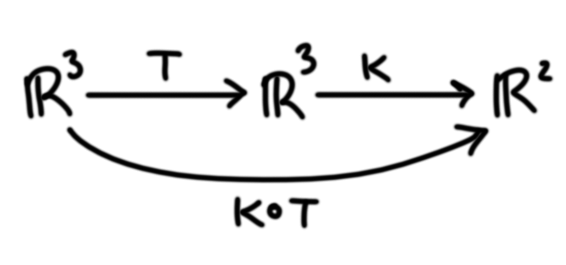
\includegraphics[scale= 1.8]{18} 
	\end{marginfigure}
	\item Usa las fórmulas de estas composiciones para calcular
	las matrices $[K \circ U]_{\delta}^{\phi}$ y 
	$[K \circ T]_{\beta}^{\phi}$.
	\item Calcula las matrices del inciso anterior usando
	representaciones matriciales apropiadas de $T$, $U$ y $K$
	y multiplicándolas entre sí.
\end{itemize}

\textbf{Además,} revisa los ejercicios del capítulo 2.3 del Friedberg,
pero en particular resuelve
3 y 4 de la página 93.
\newpage
\end{document}

